% Options for packages loaded elsewhere
\PassOptionsToPackage{unicode}{hyperref}
\PassOptionsToPackage{hyphens}{url}
\PassOptionsToPackage{dvipsnames,svgnames*,x11names*}{xcolor}
%
\documentclass[
  spanish,
]{book}
\usepackage{amsmath,amssymb}
\usepackage{lmodern}
\usepackage{ifxetex,ifluatex}
\ifnum 0\ifxetex 1\fi\ifluatex 1\fi=0 % if pdftex
  \usepackage[T1]{fontenc}
  \usepackage[utf8]{inputenc}
  \usepackage{textcomp} % provide euro and other symbols
\else % if luatex or xetex
  \usepackage{unicode-math}
  \defaultfontfeatures{Scale=MatchLowercase}
  \defaultfontfeatures[\rmfamily]{Ligatures=TeX,Scale=1}
\fi
% Use upquote if available, for straight quotes in verbatim environments
\IfFileExists{upquote.sty}{\usepackage{upquote}}{}
\IfFileExists{microtype.sty}{% use microtype if available
  \usepackage[]{microtype}
  \UseMicrotypeSet[protrusion]{basicmath} % disable protrusion for tt fonts
}{}
\makeatletter
\@ifundefined{KOMAClassName}{% if non-KOMA class
  \IfFileExists{parskip.sty}{%
    \usepackage{parskip}
  }{% else
    \setlength{\parindent}{0pt}
    \setlength{\parskip}{6pt plus 2pt minus 1pt}}
}{% if KOMA class
  \KOMAoptions{parskip=half}}
\makeatother
\usepackage{xcolor}
\IfFileExists{xurl.sty}{\usepackage{xurl}}{} % add URL line breaks if available
\IfFileExists{bookmark.sty}{\usepackage{bookmark}}{\usepackage{hyperref}}
\hypersetup{
  pdftitle={Modelos Bayesianos con R y STAN},
  pdfauthor={Andrés Gutiérrez - Hanwen Zhang},
  pdflang={es},
  colorlinks=true,
  linkcolor=blue,
  filecolor=Maroon,
  citecolor=Blue,
  urlcolor=Blue,
  pdfcreator={LaTeX via pandoc}}
\urlstyle{same} % disable monospaced font for URLs
\usepackage{color}
\usepackage{fancyvrb}
\newcommand{\VerbBar}{|}
\newcommand{\VERB}{\Verb[commandchars=\\\{\}]}
\DefineVerbatimEnvironment{Highlighting}{Verbatim}{commandchars=\\\{\}}
% Add ',fontsize=\small' for more characters per line
\usepackage{framed}
\definecolor{shadecolor}{RGB}{248,248,248}
\newenvironment{Shaded}{\begin{snugshade}}{\end{snugshade}}
\newcommand{\AlertTok}[1]{\textcolor[rgb]{0.94,0.16,0.16}{#1}}
\newcommand{\AnnotationTok}[1]{\textcolor[rgb]{0.56,0.35,0.01}{\textbf{\textit{#1}}}}
\newcommand{\AttributeTok}[1]{\textcolor[rgb]{0.77,0.63,0.00}{#1}}
\newcommand{\BaseNTok}[1]{\textcolor[rgb]{0.00,0.00,0.81}{#1}}
\newcommand{\BuiltInTok}[1]{#1}
\newcommand{\CharTok}[1]{\textcolor[rgb]{0.31,0.60,0.02}{#1}}
\newcommand{\CommentTok}[1]{\textcolor[rgb]{0.56,0.35,0.01}{\textit{#1}}}
\newcommand{\CommentVarTok}[1]{\textcolor[rgb]{0.56,0.35,0.01}{\textbf{\textit{#1}}}}
\newcommand{\ConstantTok}[1]{\textcolor[rgb]{0.00,0.00,0.00}{#1}}
\newcommand{\ControlFlowTok}[1]{\textcolor[rgb]{0.13,0.29,0.53}{\textbf{#1}}}
\newcommand{\DataTypeTok}[1]{\textcolor[rgb]{0.13,0.29,0.53}{#1}}
\newcommand{\DecValTok}[1]{\textcolor[rgb]{0.00,0.00,0.81}{#1}}
\newcommand{\DocumentationTok}[1]{\textcolor[rgb]{0.56,0.35,0.01}{\textbf{\textit{#1}}}}
\newcommand{\ErrorTok}[1]{\textcolor[rgb]{0.64,0.00,0.00}{\textbf{#1}}}
\newcommand{\ExtensionTok}[1]{#1}
\newcommand{\FloatTok}[1]{\textcolor[rgb]{0.00,0.00,0.81}{#1}}
\newcommand{\FunctionTok}[1]{\textcolor[rgb]{0.00,0.00,0.00}{#1}}
\newcommand{\ImportTok}[1]{#1}
\newcommand{\InformationTok}[1]{\textcolor[rgb]{0.56,0.35,0.01}{\textbf{\textit{#1}}}}
\newcommand{\KeywordTok}[1]{\textcolor[rgb]{0.13,0.29,0.53}{\textbf{#1}}}
\newcommand{\NormalTok}[1]{#1}
\newcommand{\OperatorTok}[1]{\textcolor[rgb]{0.81,0.36,0.00}{\textbf{#1}}}
\newcommand{\OtherTok}[1]{\textcolor[rgb]{0.56,0.35,0.01}{#1}}
\newcommand{\PreprocessorTok}[1]{\textcolor[rgb]{0.56,0.35,0.01}{\textit{#1}}}
\newcommand{\RegionMarkerTok}[1]{#1}
\newcommand{\SpecialCharTok}[1]{\textcolor[rgb]{0.00,0.00,0.00}{#1}}
\newcommand{\SpecialStringTok}[1]{\textcolor[rgb]{0.31,0.60,0.02}{#1}}
\newcommand{\StringTok}[1]{\textcolor[rgb]{0.31,0.60,0.02}{#1}}
\newcommand{\VariableTok}[1]{\textcolor[rgb]{0.00,0.00,0.00}{#1}}
\newcommand{\VerbatimStringTok}[1]{\textcolor[rgb]{0.31,0.60,0.02}{#1}}
\newcommand{\WarningTok}[1]{\textcolor[rgb]{0.56,0.35,0.01}{\textbf{\textit{#1}}}}
\usepackage{longtable,booktabs,array}
\usepackage{calc} % for calculating minipage widths
% Correct order of tables after \paragraph or \subparagraph
\usepackage{etoolbox}
\makeatletter
\patchcmd\longtable{\par}{\if@noskipsec\mbox{}\fi\par}{}{}
\makeatother
% Allow footnotes in longtable head/foot
\IfFileExists{footnotehyper.sty}{\usepackage{footnotehyper}}{\usepackage{footnote}}
\makesavenoteenv{longtable}
\usepackage{graphicx}
\makeatletter
\def\maxwidth{\ifdim\Gin@nat@width>\linewidth\linewidth\else\Gin@nat@width\fi}
\def\maxheight{\ifdim\Gin@nat@height>\textheight\textheight\else\Gin@nat@height\fi}
\makeatother
% Scale images if necessary, so that they will not overflow the page
% margins by default, and it is still possible to overwrite the defaults
% using explicit options in \includegraphics[width, height, ...]{}
\setkeys{Gin}{width=\maxwidth,height=\maxheight,keepaspectratio}
% Set default figure placement to htbp
\makeatletter
\def\fps@figure{htbp}
\makeatother
\setlength{\emergencystretch}{3em} % prevent overfull lines
\providecommand{\tightlist}{%
  \setlength{\itemsep}{0pt}\setlength{\parskip}{0pt}}
\setcounter{secnumdepth}{5}
\usepackage{booktabs}
\usepackage{setspace}
\def\bPi{\boldsymbol \Pi }
\def\bGamma{\boldsymbol \Gamma}
\def\bgamma{\boldsymbol \gamma}
\def\beps{\boldsymbol \varepsilon}
\def\bbeta{\boldsymbol \beta}
\def\bLambda{\boldsymbol \Lambda}
\def\blambda{\boldsymbol \lambda}
\def\bBeta{\boldsymbol \Beta}
\def\bEta{\boldsymbol \eta}
\def\balpha{\boldsymbol \alpha}
\def\btheta{\boldsymbol \theta}
\def\bmu{\boldsymbol \mu}
\def\bSigma{\boldsymbol \Sigma}
\def\bphi{\boldsymbol \phi}
\def\bpi{\boldsymbol \pi}
\def\bxi{\boldsymbol \xi}
\ifxetex
  % Load polyglossia as late as possible: uses bidi with RTL langages (e.g. Hebrew, Arabic)
  \usepackage{polyglossia}
  \setmainlanguage[]{spanish}
\else
  \usepackage[main=spanish]{babel}
% get rid of language-specific shorthands (see #6817):
\let\LanguageShortHands\languageshorthands
\def\languageshorthands#1{}
\fi
\ifluatex
  \usepackage{selnolig}  % disable illegal ligatures
\fi
\usepackage[]{natbib}
\bibliographystyle{apalike}

\title{Modelos Bayesianos con R y STAN}
\author{Andrés Gutiérrez - Hanwen Zhang}
\date{2021-06-05}

\usepackage{amsthm}
\newtheorem{theorem}{Teorema}[chapter]
\newtheorem{lemma}{Lema}[chapter]
\newtheorem{corollary}{Corolario}[chapter]
\newtheorem{proposition}{Resultado}[chapter]
\newtheorem{conjecture}{Conjectura}[chapter]
\theoremstyle{definition}
\newtheorem{definition}{Definición}[chapter]
\theoremstyle{definition}
\newtheorem{example}{Ejemplo}[chapter]
\theoremstyle{definition}
\newtheorem{exercise}{Ejercicio}[chapter]
\theoremstyle{definition}
\newtheorem{hypothesis}{Hipótesis}[chapter]
\theoremstyle{remark}
\newtheorem*{remark}{Comentario}
\newtheorem*{solution}{Solución}
\begin{document}
\maketitle

{
\hypersetup{linkcolor=}
\setcounter{tocdepth}{1}
\tableofcontents
}
\hypertarget{prefacio}{%
\chapter*{Prefacio}\label{prefacio}}
\addcontentsline{toc}{chapter}{Prefacio}

\hypertarget{antes-de-comenzar}{%
\chapter*{Antes de comenzar}\label{antes-de-comenzar}}
\addcontentsline{toc}{chapter}{Antes de comenzar}

\hypertarget{cuestionamientos-sobre-el-enfoque-bayesiano}{%
\section*{Cuestionamientos sobre el enfoque bayesiano}\label{cuestionamientos-sobre-el-enfoque-bayesiano}}
\addcontentsline{toc}{section}{Cuestionamientos sobre el enfoque bayesiano}

\citet{GelmanObjections} presenta algunos de los cuestionamientos que algunos estadísticos anti-bayesianos han argumentado en contra de este paradigma que, sin lugar a dudas, ha proporcionado una valiosa herramienta de modelación en la ciencia contemporanea. Revisemos algunos de estos argumentos:

\begin{quote}
La inferencia bayesiana es una teoría matemática coherente pero no brinda la suficiente confianza en usos científicos. Las distribuciones \emph{previas} subjetivas no inspiran confianza porque ni siquiera existe algún principio objetivo para elegir una distribución previa no informativa. ¿De dónde vienen las distribuciones previas? No confío en ellas y no veo ninguna razón para recomendarlas a otra gente, apenas me siento cómodo acerca de su coherencia filosófica.
\end{quote}

Este argumento es débil puesto que la teoría bayesiana es una teoría cinetífica apoyada en los axiomas matemáticos de la teoría de la medida y de probabilidad. De la mismaforma, nótese que tampoco existe un principio objetivo para escoger una verosimilitud. ¿De dónde vienen las regresiones logísticas? ¿quién dijo que los datos eran normales? Como toda ciencia, la estadística se basa en procedimientos subjetivos que inducen resultados que se pueden probar de una manera objetiva. Al decidir usar una determinada distribución previa, el investigador está haciendo uso de su conocimiento objetivo sobre el fenómeno de interés. Esto no dista mucho de la planificación de un estudio por muestreo o de un experimento, en donde se hace uso de la información auxiliar disponible para definir la mejor versión del estudio. Además, como se verá más adelante, sí existen principios objetivos que permiten decidir acerca de la elección de una distribución previa; por ejemplo, la invarianza de la distribución previa frente a transformaciones de los parámetros.

\begin{quote}
La teoría bayesiana requiere un pensamiento mucho más profundo sobre la situación y recomendarle a los investigadores comunes el uso del teorema de Bayes es como darle al hijo del vecino la llave de un \emph{F-16}. De veras que, yo comenzaría con algo de métodos probados y confiables, y entonces generalizaría la situación utilizando los principios estadísticos y la teoría del minimax, que no dependen de ninguna creencia subjetiva. Especialmente cuando las distribuciones previas que veo en la práctica toman formas conjugadas. ¡Qué coincidencia!
\end{quote}

Como científicos e investigadores debemos tratar con el conocimiento objetivo y dejar a un lado las creencias subjetivas. Es por eso que las distribuciones previas que se manejan en la inferencia bayesiana son objetivas de la misma forma que lo son los métodos frecuentistas al asignar un modelo probabilístico a la verosimilitud de los datos. El resultado final sólo depende del modelo asumido y de los datos recolectados. A pesar de que algunos resultados de la inferencia bayesiana coinciden con el acercamiento frecuentista, esto no sucede en todos los casos. Si la distribución es conjugada, simplemente quiere decir que es posible utilizar un generador de números aleatorios conocido; sin embargo, en pleno siglo XXI, esto ya no constituye un problema.

\begin{quote}
Dejando de lado las preocupaciones matemáticas, me gustan las estimaciones insesgadas, los intervalos de confianza con un nivel real de cobertura. Pienso que la manera correcta de inferir es acercarse al parámetro tanto como sea posible y desarrollar métodos robustos que trabajen con supuestos mínimos. El acercamiento bayesiano intenta aproximar el insesgamiento, mientras asume supuestos más y más fuertes. En los viejos tiempos, los métodos Bayesianos por lo menos tenían la virtud de estar matemáticamente limpios. Hoy en día, cualquier inferencia se realiza mediante el uso de las cadenas de Markov con métodos de Monte Carlo (MCMC). Lo anterior significa que, no sólo no se pueden evaluar las características estadísticas del método, sino que tampoco se puede asegurar su convergencia.
\end{quote}

Los métodos bayesianos parecen moverse rápidamente hacia la computación elaborada. Para bien o para mal, la computación se está convirtiendo en una plataforma central para el desarrollo científico y estadístico. Por otro lado, estos mismos adelantos de computación científica permiten evaluar las características de los modelos bayesianos y la convergencia de las cadenas de la distribución posterior. Haciendo uso de la rigurosidad científica, el investigador debe conocer a profundidad el espíritu de los métodos MCMC y verificar que la distribución posterior conjunta sobre un vector de parámetros no sea impropia, y por supuesto verificar que las cadenas tienen propiedades estacionarias.

\begin{quote}
La gente tiende a creer los resultados que apoyan sus preconceptos y descreen los resultados que los sorprenden, ésta es una forma errada y sesgada de pensar. Pues bien, los métodos bayesianos animan este modo indisciplinado de pensamiento. Estoy seguro que muchos estadísticos bayesianos están actuando de buena fe; sin embargo, al mismo tiempo, también están proporcionando estímulo a investigadores descuidados y poco éticos por todas partes, porque el investigador queda estancado al momento de escoger una distribución previa.
\end{quote}

Si hay una seria diferenciación entre las creencias subjetivas y los resultados posteriores, debería ser un indicador de revaluar el modelo usado. Además, ante el desconocimiento del fenómeno, el investigador bayesiano puede utilizar una distribución previa débil y añadir más información si se necesita. Las verificaciones predictivas (previas y posteriores) son una parte esencial del método bayesiano que obliga a repensar las creencias del investigador con respecto al parámetro de interés. Este ejercicio redunda en el replanteamineto de la distribución previa mediante el estudio de las distribuciones predictivas, decantándose al final por el mejor modelo.

\begin{quote}
Los cálculos de la teoría de la decisión guían a la idea de que el muestreo probabilístico y la asignación aleatoria de tratamientos son ineficaces, de que los mejores diseños y muestras son los determinísticos. No tengo ningún conflicto con estos cálculos matemáticos; el conflicto es más profundo, en los fundamentos filosóficos, en la idea de que el objetivo de la estadística consiste en tomar una decisión óptima. Un estimador bayesiano es un estimador estadístico que reduce al mínimo el riesgo promedio. Sin embargo, cuando hacemos estadística, no estamos intentando \emph{reducir al mínimo el riesgo promedio}, estamos intentando hacer estimación y juzgamiento de hipótesis.
\end{quote}

Un estimador bayesiano es un estimador estadístico que minimiza el riesgo promedio. Uno de los primeros tópicos que se presentan en este libro es el de la teoría de la decisión y funciones de perdida, como herramientas fundamentales del aprendizaje estadístico \citep{hastie}. Además, como se verá más adelante, la asignación de las unidades experimentales al tratamiento o la inclusión de las unidades muestrales en un estudio probabilístico debe y puede ser tenido en cuenta en los modelos bayesianos, mediante la inclusión en el modelo de las variables que intervinieron en la selección de las unidades. De la misma forma, el juzgamiento de hipótesis es una práctica que se extiende en la modelación bayesiana.

\begin{quote}
No puedo estar al tanto de lo que están haciendo todos esos Bayesianos hoy en día. Desafortunadamente, toda clase de personas están siendo seducidas por las promesas de la inferencia automática con la \emph{magia del MCMC}. Desearía que todos paráramos de una vez y por todas y empezáramos, de nuevo, a hacer estadística de la forma en que debe ser hecha: volviendo a los viejos tiempos en que un \(p\)-valor era utilizado para algo, cuando un intervalo de confianza tenía significado, y el sesgo estadístico era algo que se quería eliminar y no algo que se debiera abrazar.
\end{quote}

Los métodos Bayesianos algunas veces son presentados como un motor de inferencia automática. Sin embargo, la inferencia bayesiana tiene tres etapas: formulación del modelo, ajuste del modelo a los datos, evaluación del ajuste. Así que el procedimiento no es mágico ni automático. Además, una de las ventajas de la estadística bayesiana es que deja de lado las sofisticaciones de la inferencia clásica en donde, por ejemplo, la simple interpretación de un intervalo de confianza se hace muy complicada a la luz del razonamiento lógico. De la misma forma los valores \(p\) constituyen un paradigma cada vez más revalorado en la investigación social.

\hypertarget{acerca-de-la-notaciuxf3n}{%
\section*{Acerca de la notación}\label{acerca-de-la-notaciuxf3n}}
\addcontentsline{toc}{section}{Acerca de la notación}

Antes de empezar las próximas secciones, es necesario revisar la
notación que se seguirá de ahora en adelante. Del teorema de Bayes
resultan tres grandes definiciones que constituyen la base de la
estadística Bayesiana y que a lo largo de este texto se mencionarán
diferenciándolas por medio de la notación. El símbolo más importante de
la estadística matemática es \(p\), el cual indica que existe una
distribución de probabilidad para los datos, para el vector de
parámetros, condicional o no. De hecho todos las definiciones y
resultados anteriores han estado supeditadas al uso de esta monótona
notación. En el ámbito de la notación de investigación internacional es
común diferenciar las distribuciones con el fin de hacer más ameno el
estudio del enfoque Bayesiano. En este texto se seguirá esta distinción.
Un ejemplo claro en donde \(p\) representa cuatro funciones distintas en
una sola ecuación es el siguiente:

\[p(\theta \mid y)=p(y \mid \theta)\frac{p(\theta)}{p(y)}\]

\citet{Gelman95} explica por qué la notación simple, con el uso (a
veces abuso) de la letra \(p\) es más rigurosa de lo que, a simple vista,
pueda parecer y comenta que,

\begin{quote}
En realidad no me gusta la notación que la mayoría de los estadísticos usen \(f\) para las distribuciones de muestreo; \(\pi\), para las distribuciones previas y \(L\), para las verosimilitudes. Este estilo de notación se desvía de lo que realmente es importante. La notación no debería depender del orden en que las distribuciones son especificadas. Todas ellas son distribuciones de probabilidad, eso es lo realmente importante.
\end{quote}

Esto tiene sentido, aún más cuando se estudian las propiedades
estadísticas de los estimadores desde el punto de vista de la teoría de
la medida. Siendo así, el símbolo \(p\) se refiere a una notación para una
medida de probabilidad, quizás inducida por un elemento aleatorio. De
hecho, en la ecuación que determina la regla de Bayes, cada una de las
\(p\) son medidas de probabilidad que no comparten el mismo espacio de
medida (ni la misma \(\sigma\)-álgebra, ni el mismo espacio muestral).

De hecho, todo queda claro al realizar un diagrama que permita ver el
espacio de salida y el espacio de llegada de los elementos aleatorios
que inducen (si es el caso), cada una de las distribuciones de
probabilidad. Por otra parte, Bob Carpenter concluye que:

\begin{quote}
Una vez resuelto el problema de identificación de los espacios, la notación estadística depende en gran manera del contexto y aunque la regla de Bayes no necesite de mucha explicación, es necesario conocerlo todo acerca del contexto para poder interpretar las funciones que la conforman\ldots{} El problema se hace mucho más agudo para los estadísticos novatos, pero eso se resuelve con la práctica. Una vez que uno sabe lo que está haciendo, se vuelve obvia la referencia de la distribución \(p\).
\end{quote}

Por lo anterior, es natural que algunos de los textos clásicos de
estadística matemática, los autores asumen que el lector sigue la idea
de la referencia de la distribución \(p\) en cuestión.

\hypertarget{tuxf3picos-buxe1sicos}{%
\chapter{Tópicos básicos}\label{tuxf3picos-buxe1sicos}}

\hypertarget{teoruxeda-de-la-decisiuxf3n}{%
\section{Teoría de la decisión}\label{teoruxeda-de-la-decisiuxf3n}}

El problema estadístico de estimar un parámetro se puede ver dentro del contexto de la teoría de decisión: la estimación que proveemos, sea en el ámbito de la estadística clásica o la estadística bayesiana, depende de los datos muestrales, \(\mathbf{X}\), de tal forma que si éstos cambian, la estimación también cambia. De esta manera, el proceso de estimación puede ser representado como una función que toma un conjunto de datos muestrales y los convierte en una estimación (\(A(\mathbf{X})\) o simplemente \(A\)) del parámetro de interés. En la teoría de decisión, la anterior función se conoce como una regla de decisión.

Así como en la vida cotidiana, por la incertidumbre del futuro (en el ámbito estadístico, por la incertidumbre acerca del parámetro), toda acción que se tome (toda estimación que se provea) puede traer consigo un grado de falla o riesgo. Y es necesario escoger la acción óptima que de alguna forma minimice ese riesgo. Formalizando esta idea intuitiva, se define la función de pérdida \(L\) que asocia a cada dupla conformada por la acción tomada y el parámetro de interés \(\theta\), \((A, \ \theta)\) con un número no negativo que cuantifica la pérdida que ocasiona la acción (o la estimación) \(A\) con respecto al parámetro \(\theta\).

Es claro que se desea escoger aquella acción que minimice de alguna forma la pérdida que ésta ocasiona, pero la función \(L\) no se puede minimizar directamente, puesto que:

\begin{itemize}
\item
  En el ámbito de la estadística clásica, el parámetro \(\theta\) se considera fijo, y los datos muestrales \(\mathbf{X}\) aleatorios. Como la función de pérdida \(L\) depende de \(\mathbf{X}\), entonces ésta también será una variable aleatoria, y no se puede minimizar directamente. Por lo tanto se define el riesgo o la pérdida promedio como la esperanza matemática de \(L\); denotando el riesgo como \(R\), éste está definido como \(R=E(L)\) (la esperanza se toma con respecto a la distribución probabilística de \(\mathbf{X}\)).
\item
  En el ámbito de la estadística bayesiana, \(\theta\) sigue siendo una cantidad fija, pero la incertidumbre que tiene el investigador sobre la localización del parámetro se puede modelar mediante funciones de probabilidad. La herramienta fundamental para conocer características de \(\theta\) es su función de densidad posterior \(p(\theta|\mathbf{X})\). En este caso, el riesgo \(R\) se define como
\end{itemize}

\begin{equation*}
R=E(L)=\int L(A, \theta)p(\theta|\mathbf{X})d\theta
\end{equation*}

En cualquiera de los dos casos anteriores, se busca la estimación que minimice el riesgo \(R\). Ilustramos los anteriores conceptos en los siguientes ejemplos tanto en la estadística clásica como en la estadística bayesiana.

\begin{example}
\protect\hypertarget{exm:unnamed-chunk-1}{}{\label{exm:unnamed-chunk-1} }Sea \(X_i\) con \(i=1,\cdots, n\) una muestra aleatoria con media \(\theta\) y varianza \(\sigma^2\), ambas fijas, y suponga que se desea encontrar el mejor estimador de \(\theta\) bajo la función de pérdida cuadrática dada por

\begin{equation*}
L(A,\theta)=(A-\theta)^2
\end{equation*}

cuyo riesgo asociado está dado por \(R=E(A-\theta)^2\). En primer lugar, buscaremos dicho estimador dentro de todas las formas lineales de \(X_i\), es decir, los estimadores de la forma \(A=\sum_{i=1}^nc_iX_i\). Por tanto, el riesgo se puede expresar como
\begin{align*}
R=E(A-\theta)^2&=Var(A)+(E(A)-\theta)^2\\
&=\sum_{i=1}^nc_i^2\sigma^2+\theta^2(\sum_{i=1}^nc_i-1)^2
\end{align*}

Y al buscar los coeficientes \(c_i\) que minimizan la anterior expresión, encontramos que \(c_i=\theta^2/(\sigma^2+n\theta^2)\) para todo \(i\). Como estos coeficientes conducen a un estimador que depende del parámetro desconocido, concluimos que no hay ningún estimador que minimiza el riesgo.

Para encontrar una solución, es necesario restringir aún más el rango de estimadores; para eso, se impone la restricción de que \(\sum_{i=1}^n c_i=1\). De esta forma, el riesgo está dado por \(R=\sum c_i^2\sigma^2\). Dado que \(\sigma^2\) es fijo, al minimizar \(\sum c_i^2\) sujeto a la restricción, se tiene que la solución es \(c_i=1/n\) para todo \(i\), y así encontramos que el mejor estimador (en el sentido de minimizar el riesgo de la función de pérdida cuadrática) dentro de todas las formas lineales con \(\sum c_i=1\) es la media muestral \(\bar{X}\).
\end{example}

\begin{example}
\protect\hypertarget{exm:unnamed-chunk-2}{}{\label{exm:unnamed-chunk-2} }Suponga que se desea estimar un parámetro de interés \(\theta\) en el contexto de la estadística bayesiana y denotamos la función de densidad posterior de \(\theta\) como \(p(\theta|\mathbf{X})\), entonces si utilizamos la función de pérdida cuadrática, el riesgo asociado será

\begin{align*}
R&=E(L(A,\theta))=E (A-\theta)^2=Var(\theta)+(E(\theta)-A)^2
\end{align*}

que es minimizado si \(A=E(\theta)\). Es decir, la mejor acción para estimar \(\theta\) es utilizar su tomada con respecto a la distribución posterior \(p(\theta|\mathbf{X})\).
\end{example}

\begin{example}
\protect\hypertarget{exm:unnamed-chunk-3}{}{\label{exm:unnamed-chunk-3} }En el mismo contexto del ejemplo anterior, si cambiamos la función de pérdida a la siguiente
\begin{equation*}
L(A,\theta)=|A-\theta|=(A-\theta)I_{(A\geq\theta)}+(\theta-A)I_{(\theta>A)}
\end{equation*}

El riesgo estará dado por
\begin{align*}
R&=E(L(A,\theta))\\
&=\int L(A,\theta)p(\theta|\mathbf{X})d\theta\\
&=\int_{(A\geq\theta)}(A-\theta)p(\theta|\mathbf{X})d\theta+\int_{(\theta>A)}(\theta-A)p(\theta|\mathbf{X})d\theta
\end{align*}

Derivando el riesgo con respecto a la acción \(A\), se tiene que
\begin{equation*}
\frac{\partial R}{\partial A}=\int_{(A\geq\theta)}p(\theta|\mathbf{X})d\theta-\int_{(\theta>A)}p(\theta|\mathbf{X})d\theta
\end{equation*}

Igualando a cero, tenemos que
\begin{equation*}
\int_{(A\geq\theta)}p(\theta|\mathbf{X})d\theta=\int_{(\theta>A)}p(\theta|\mathbf{X})d\theta=0.5
\end{equation*}

Y concluimos que la acción \(A\) que induce menor riesgo corresponde al percentil 50\% o la mediana de la distribución posterior de \(\theta\).
\end{example}

De los anteriores ejemplos se observa que, bajo un mismo contexto, cuando se utilizan diferentes funciones de pérdida, también se obtienen distintas estimaciones, y distintas acciones que optimizan el riesgo.

\hypertarget{algunos-resultados-de-probabilidad}{%
\section{Algunos resultados de probabilidad}\label{algunos-resultados-de-probabilidad}}

Antes de entrar en el repaso de estos conceptos fundamentales, se definen los conceptos de \textbf{parámetro} y \textbf{espacio paramétrico} asociados a una distribución de probabilidad.

\begin{enumerate}
\def\labelenumi{\arabic{enumi}.}
\tightlist
\item
  Un parámetro es aquella cantidad que define la forma funcional de una distribución de probabilidad; es decir, cuando el parámetro cambia de valor, la función de densidad y la función de distribución cambian. Las distribuciones de probabilidad pueden tener más de un parámetro. Cuando una distribución tiene solo un parámetro, éste se denota usualmente por \(\theta\), cuando se presenta más de un parámetro, la notación se cambia a \(\boldsymbol \theta\), representando el vector de parámetros.
\item
  El espacio paramétrico, \(\Theta\), es el conjunto que contiene todos los posibles valores que puede tomar el parámetro o el vector de parámetros. Para distribuciones con un solo parámetro, \(\Theta\) será un subconjunto de \(\mathbb{R}\), mientras que para distribuciones con dos o más parámetros, \(\Theta\) será un subconjunto de \(\mathbb{R}\times\mathbb{R}\).
\end{enumerate}

Para entender los fundamentos de la modelación bayesiana, es necesario
recordar algunas definiciones y resultados de la teoría de probabilidad
que ayudarán a hacer más expedito este periplo por la estadística
bayesiana. En términos de notación, se utilizará indistintamente la
expresión de integral, \(\int\), indicando la sumatoria, en el caso de las
variables aleatorias discretas o la integral de Riemann-Stieltjes en el
caso de las variables aleatorias continuas.

\begin{definition}
\protect\hypertarget{def:unnamed-chunk-4}{}{\label{def:unnamed-chunk-4} }Sean \(\mathbf{X}=(X_1,\ldots,X_p)'\), \(\mathbf{Y}=(Y_1,\ldots,Y_q)'\) dos vectores aleatorios definidos sobre los espacios de muestreo \(\mathcal{X}\), \(\mathcal{Y}\), respectivamente. Suponga que la distribución conjunta de estos vectores aleatorios está dada por \(p(\mathbf{X},\mathbf{Y})\). La distribución marginal de \(\mathbf{X}\) está dada por
\begin{equation}
p(\mathbf{X})=\int p(\mathbf{X},\mathbf{Y})\ d\mathbf{Y}
\end{equation}
y la distribución condicional de \(\mathbf{X}\) dado \(\mathbf{Y}\) como
\begin{equation}
p(\mathbf{X} \mid \mathbf{Y})
=\frac{p(\mathbf{X},\mathbf{Y})}{p(\mathbf{Y})}
\end{equation}
\end{definition}

\begin{proposition}
\protect\hypertarget{prp:Res121}{}{\label{prp:Res121} }Suponga los vectores \(\mathbf{X}\), \(\mathbf{Y}\) y un tercer vector \(\mathbf{Z}=(Z_1,\ldots,Z_r)'\) definido sobre el espacio de muestreo \(\mathcal{Z}\). Entonces se tiene que
\begin{equation}
p(\mathbf{X} \mid \mathbf{Z})=\int p(\mathbf{X},\mathbf{Y} \mid \mathbf{Z})\ d\mathbf{Y}
\end{equation}
y
\begin{equation}
p(\mathbf{X} \mid \mathbf{Y},\mathbf{Z})=\frac{p(\mathbf{X},\mathbf{Y} \mid \mathbf{Z})}{p(\mathbf{Y} \mid \mathbf{Z})}
\end{equation}
\end{proposition}

\begin{proof}
\iffalse{} {Prueba. } \fi{}En primer lugar, nótese que
\begin{align*}
\int p(\mathbf{X},\mathbf{Y} \mid \mathbf{Z})\ d\mathbf{Y}&=
\int \frac{p(\mathbf{X},\mathbf{Y},\mathbf{Z})}{p(\mathbf{Z})}\ d\mathbf{Y}\\
&=\frac{1}{p(\mathbf{Z})} \int p(\mathbf{X},\mathbf{Y},\mathbf{Z}) \ d\mathbf{Y}\\
&=\frac{1}{p(\mathbf{Z})} p(\mathbf{X},\mathbf{Z})=p(\mathbf{X} \mid \mathbf{Z})
\end{align*}

Por otro lado,

\begin{align*}
\frac{p(\mathbf{X},\mathbf{Y} \mid \mathbf{Z})}{p(\mathbf{Y} \mid \mathbf{Z})}=
\frac{p(\mathbf{X},\mathbf{Y},\mathbf{Z})}{p(\mathbf{Z})} \diagup
\frac{p(\mathbf{Y},\mathbf{Z})}{p(\mathbf{Z})}
=\frac{p(\mathbf{X},\mathbf{Y},\mathbf{Z})}{p(\mathbf{Y},\mathbf{Z})}=p(\mathbf{X} \mid \mathbf{Y},\mathbf{Z})
\end{align*}
\end{proof}

\begin{definition}
\protect\hypertarget{def:unnamed-chunk-6}{}{\label{def:unnamed-chunk-6} }Sean \(\mathbf{X}\), \(\mathbf{Y}\), \(\mathbf{Z}\) vectores aleatorios, se dice que \(\mathbf{X}\) es condicionalmente independiente de \(\mathbf{Y}\) con respecto a \(\mathbf{Z}\) si satisfacen la siguiente expresión
\begin{equation}
p(\mathbf{X},\mathbf{Y} \mid \mathbf{Z})=p(\mathbf{X} \mid \mathbf{Z})p(\mathbf{Y} \mid \mathbf{Z})
\end{equation}
\end{definition}

\begin{proposition}
\protect\hypertarget{prp:Res122}{}{\label{prp:Res122} }Si \(\mathbf{X}\) es condicionalmente independiente de \(\mathbf{Y}\) con respecto a \(\mathbf{Z}\), entonces se tiene que
\begin{equation}
p(\mathbf{X} \mid \mathbf{Y},\mathbf{Z})=p(\mathbf{X} \mid \mathbf{Z})
\end{equation}
\end{proposition}

\begin{proof}
\iffalse{} {Prueba. } \fi{}Como \(p(\mathbf{X},\mathbf{Y} \mid \mathbf{Z})=\dfrac{p(\mathbf{X},\mathbf{Y},\mathbf{Z})}{p(\mathbf{Z})}\), entonces

\begin{align*}
p(\mathbf{X} \mid \mathbf{Y},\mathbf{Z})=\frac{p(\mathbf{X},\mathbf{Y},\mathbf{Z})}{p(\mathbf{Y},\mathbf{Z})}
=\frac{p(\mathbf{X},\mathbf{Y} \mid \mathbf{Z})p(\mathbf{Z})}{p(\mathbf{Y},\mathbf{Z})}
=\frac{p(\mathbf{X} \mid \mathbf{Z})p(\mathbf{Y} \mid \mathbf{Z})}{p(\mathbf{Y} \mid \mathbf{Z})}=p(\mathbf{X} \mid \mathbf{Z})
\end{align*}
\end{proof}

\begin{proposition}
\protect\hypertarget{prp:unnamed-chunk-8}{}{\label{prp:unnamed-chunk-8} }Si \(\mathbf{X}\) es independiente de \(\mathbf{Y}\), entonces \(\mathbf{X}\) es condicionalmente independiente de \(\mathbf{Y}\) dado cualquier otro vector \(\mathbf{Z}\).
\end{proposition}

\begin{proof}
\iffalse{} {Prueba. } \fi{}Nótese que
\begin{equation*}
p(\mathbf{X},\mathbf{Y}\mid \mathbf{Z})=p(\mathbf{X} \mid \mathbf{Y},\mathbf{Z})p(\mathbf{Y} \mid \mathbf{Z})=p(\mathbf{X} \mid \mathbf{Z})p(\mathbf{Y} \mid \mathbf{Z})
\end{equation*}

puesto que, utilizando la hipótesis de independencia, se tiene que
\begin{equation*}
p(\mathbf{X} \mid \mathbf{Y})=p(\mathbf{X})
\end{equation*}
\end{proof}

\hypertarget{teorema-de-bayes}{%
\section{Teorema de Bayes}\label{teorema-de-bayes}}

Desde la revolución estadística de Pearson y Fisher, la inferencia
estadística busca encontrar los valores que parametrizan a la
distribución desconocida de los datos. El primer enfoque, propuesto por
Pearson, afirmaba que si era posible observar a la variable de interés
en todos y cada uno de los individuos de una población, entonces era
posible calcular los parámetros de la distribución de la variable de
interés; por otro lado, si solo se tenía acceso a una muestra
representativa, entonces era posible calcular una estimación de tales
parámetros. Sin embargo, Fisher discrepó de tales argumentos, asumiendo
que las observaciones están sujetas a un error de medición y por lo
tanto, así se tuviese acceso a toda la población, sería imposible calcular
los parámetros de la distribución de la variable de interés.

Del planteamiento de Fisher resultaron una multitud de métodos
estadísticos para la estimación de los parámetros poblacionales. Es
decir, si la distribución de \(\mathbf{Y}\) está parametrizada por
\(\boldsymbol \theta=(\theta_1,\ldots,\theta_K)\), \(\boldsymbol \theta\in \Theta\) con \(\Theta\)
el espacio paramétrico inducido por el comportamiento de la variable de
interés, el objetivo de la teoría estadística inferencial es calcular
una estimación \(\hat{\boldsymbol \theta}\) del parámetro \(\boldsymbol \theta\), por medio de los
datos observados. En este enfoque, los parámetros se consideran
cantidades fijas y constantes. Sin embargo, en la última mitad del siglo
XX, algunos investigadores estadísticos comenzaron a reflexionar acerca
de la naturaleza de \(\boldsymbol \theta\) y enfocaron la inferencia estadística de
una manera distinta: \emph{asumiendo que la distribución de la variable de
interés está condicionada a valores específicos de los parámetros}. Es
decir, en términos de notación, si la variable de interés es
\(\mathbf{Y}\), su distribución condicionada a los parámetros toma la
siguiente forma \(p(\mathbf{Y} \mid \boldsymbol \theta)\). Esto implica claramente
que en este nuevo enfoque la naturaleza de los parámetros no es
constante.

En términos de inferencia para \(\boldsymbol \theta\), es necesario encontrar la
distribución de los parámetros condicionada a la observación de los
datos. Para este fin, es necesario definir la distribución conjunta de
la variable de interés con el vector de parámetros.
\begin{equation*}
p(\boldsymbol \theta,\mathbf{Y})=p(\boldsymbol \theta)p(\mathbf{Y} \mid \boldsymbol \theta)
\end{equation*}

A la distribución \(p(\boldsymbol \theta)\) se le conoce con el nombre de
distribución \emph{previa} y en ella se enmarcan todas y cada una de las
creencias que se tienen acerca del comportamiento estocástico del vector
de parámetros antes de que ocurra la recolección de los datos; \(p(\mathbf{Y} \mid \boldsymbol \theta)\) es la distribución de muestreo,
verosimilitud o distribución de los datos. Por otro lado, la
distribución del vector de parámetros condicionada a los datos
observados está dada por

\begin{equation}
\label{eq:Bayes}
p(\boldsymbol \theta\mid \mathbf{Y})=\frac{p(\boldsymbol \theta,\mathbf{Y})}{p(\mathbf{Y})}=\frac{p(\boldsymbol \theta)p(\mathbf{Y} \mid \boldsymbol \theta)}{p(\mathbf{Y})}
\end{equation}

A la distribución \(p(\boldsymbol \theta\mid \mathbf{Y})\) se le conoce con el
nombre de distribución \emph{posterior} y en ella se enmarcan las
creencias actualizadas acerca del comportamiento estocástico del vector
de parámetros teniendo en cuenta los datos observados \(\mathbf{Y}\).
Nótese que la expresión \eqref{eq:Bayes} se compone de una fracción cuyo
denominador no depende del vector de parámetros y considerando a los
datos observados como fijos, corresponde a una constante y puede ser
obviada. Por lo tanto, otra representación de la regla de Bayes está
dada por

\begin{align}
\label{eq:Bayes1}
p(\boldsymbol \theta\mid \mathbf{Y})\propto p(\mathbf{Y} \mid \boldsymbol \theta)p(\boldsymbol \theta)
\end{align}

\citet{Gelman03} menciona que esta expresión se conoce como la
distribución \emph{posterior no-normalizada} y encierra el núcleo
técnico de la inferencia bayesiana. La constante \(p(\mathbf{Y})\)
faltante en la expresión \eqref{eq:Bayes1} se da a continuación.

\begin{proposition}
\protect\hypertarget{prp:Res131}{}{\label{prp:Res131} }La expresión \(p(\mathbf{Y})\) corresponde a una constante \(k\) tal que
\begin{equation*}
k=p(\mathbf{Y})=E_{\boldsymbol \theta}[p(Y \mid \boldsymbol \theta)]
\end{equation*}
\end{proposition}

\begin{proof}
\iffalse{} {Prueba. } \fi{}Nótese que
\begin{equation*}
k=p(\mathbf{Y})=\int p(\mathbf{Y},\boldsymbol \theta)\ d\boldsymbol \theta=\int p(\boldsymbol \theta)p(\mathbf{Y} \mid \boldsymbol \theta)\ d\boldsymbol \theta.
\end{equation*}
entonces
\begin{align*}
k&=\int p(\mathbf{Y} \mid \boldsymbol \theta)p(\boldsymbol \theta)\ d\boldsymbol \theta\\
&=E_{\boldsymbol \theta}[p(Y \mid \boldsymbol \theta)]
\end{align*}
\end{proof}

Curiosamente, el reverendo Thomas Bayes nunca publicó este resultado,
sino que después de su fallecimiento, su amigo el filósofo Richard
Price, encontró los escritos dentro de sus pertenencias, y éstos fueron
publicados en el 1764 en
\emph{Philosophical Transactions of the Royal Society of London}. Aunque
el teorema de Bayes fue nombrado en honor de Thomas Bayes, es casi
seguro que él mismo no sospechaba del gran impacto de su resultado. De hecho, aproximadamente una década más tarde, Pierre-Simon Laplace también descrubrió el mismo principio, y dedicó gran parte de su vida extendiéndolo y formalizándolo. Más aún, él analizó grandes volumenes de datos relacionados a los nacimientos en diferentes paises para confirmar esta teoría, y sentó las bases de la estadística bayesiana.

A continuación se presenta un ejemplo simple de este sencillo pero
poderoso teorema.

\begin{example}
\protect\hypertarget{exm:unnamed-chunk-11}{}{\label{exm:unnamed-chunk-11} }Suponga que una fábrica del sector industrial produce bolígrafos y que la producción está a cargo de tres máquinas. La primera máquina produce el 50\% del total de bolígrafos en el año, la segunda máquina produce el 30\% y la última maquina produce el restante 20\%. Por supuesto, esta producción esta sujeta al error y por tanto, basados en la experiencia, es posible reconocer que, de los artículos producidos por la primera máquina, el 5\% resultan defectuosos; de los artículos producidos por la segunda máquina, el 2\% resultan defectuosos y, de los artículos producidos por la última máquina, el 6\% resultan defectuosos.

Una pregunta natural que surge es acerca de la probabilidad de selección de un artículo defectuoso y para responder a esta pregunta con rigurosidad de probabilística es necesario enfocar la atención en los tópicos básicos que dejamos atrás. En primer lugar, el experimento en cuestión es la selección de un bolígrafo. Para este experimento, una terna \((\Omega, \mathfrak{F}, P)\) \footnote{\(\Omega\) denota el conjunto de todos lo posibles resultados del experimento, \(\mathfrak{F}\) denota una \(\sigma\)-álgebra y \(P\) hace referencia ana medida de probabilidad propiamente definida.}, llamada comúnmente espacio de medida o espacio de probabilidad, está dada por

\begin{enumerate}
\def\labelenumi{\arabic{enumi}.}
\tightlist
\item
  El espacio muestral: \(\Omega=\{\text{defectuoso}, \text{No defectouso}\}\)
\item
  La \(\sigma\)-álgebra: \(\mathfrak{F}=\{\Omega, \phi, \{\text{Defectuoso}\}, \{\text{No Defectuoso}\}\}\)
\item
  La función de probabilidad:
  \begin{align*}
    p: \mathfrak{F} &\longrightarrow [0,1]\\
    \Omega &\longrightarrow 1\\
    \phi &\longrightarrow 0\\
    \{Defectuoso\}&\longrightarrow P(D)\\
    \{No Defectuoso\}&\longrightarrow 1-P(D)
    \end{align*}
  en donde, acudiendo al teorema de probabilidad total, se define
  \begin{equation*}
    p(D)=p(D \mid M1)P(M1)+p(D \mid M2)P(M2)+p(D \mid M3)P(M3)
    \end{equation*}
\end{enumerate}

Sin embargo, también es posible plantearse otro tipo de preguntas que sirven para calibrar el proceso de producción de artículos defectuosos. Por ejemplo, cabe preguntarse acerca de la probabilidad de que, habiendo seleccionado un artículo defectuoso, éste provenga de la primera máquina\footnote{Por supuesto que la pregunta también es válida al indagar por la probabilidad de que habiendo seleccionado un artículo defectuoso, éste provenga de la segunda o tercera máquina.}. En esta ocasión, el experimento ha cambiado y ahora se trata de seleccionar un artículo defectuoso y para responder a tal cuestionamiento, se debe establecer rigurosamente el espacio de probabilidad que puede estar dado por

\begin{enumerate}
\def\labelenumi{\arabic{enumi}.}
\tightlist
\item
  El espacio muestral: \(\Omega=\{M1, M2, M3 \}\)
\item
  La \(\sigma\)-álgebra: \(\mathfrak{F}^+=\{\Omega, \phi, \{M1\}, \{M2,M3\}\}\)
\item
  La función de probabilidad:
  \begin{align*}
    p: \mathfrak{F}^+ &\longrightarrow [0,1]\\
    \Omega &\longrightarrow 1\\
    \phi &\longrightarrow 0\\
    \{M1\}&\longrightarrow p(M1 \mid D)\\
    \{M2,M3\}&\longrightarrow 1-p(M1 \mid D)
    \end{align*}
  en donde, acudiendo a la probabilidad condicional, se define
  \begin{equation*}
    p(M1 \mid D)=\frac{p(D \mid M1)P(M1)}{p(D \mid M1)P(M1)+p(D \mid M2)P(M2)+p(D \mid M3)P(M3)}
    \end{equation*}
\end{enumerate}

La anterior función de probabilidad se conoce con el nombre de regla de probabilidad de Bayes y, aparte de ser el baluarte de la mayoría de investigaciones estadísticas que se plantean hoy en día, ha sido la piedra de tropiezo de muchos investigadores radicales que trataron de estigmatizar este enfoque tildando a sus seguidores de mediocres matemáticos y pobres probabilistas afirmando que la regla de probabilidad de Bayes es sólo un artilugio diseñado para divertirse en el tablero.

Pues bien, la interpretación de la regla de bayes se puede realizar en el sentido de actualización de la estructura probabilística que gobierna el experimento. Y esta actualización tiene mucho sentido práctico cuando se cae en la cuenta de que la vida real está llena de calibradores y que las situaciones generadas son consecuencia de algún cambio estructural. De esta forma, el conocimiento de la probabilidad de que el artículo sea producido por la primera máquina se actualiza al conocer que este artículo particular es defectuoso y de esta manera calibra la estructura aleatoria que existe detrás del contexto de la fábrica de bolígrafos. Aparte de servir para resolver problemas como el anteriormente mencionado, la regla de bayes ha marcado el comienzo de un nuevo enfoque de análisis de datos, no solamente porque hace explícitas las relaciones causales entre los procesos aleatorios, sino también porque facilita la inferencia estadística y la interpretación de los resultados.
\end{example}

En el campo de la medicina, también se ha visto un gran número de la
aplicación del teorema de Bayes. A continuación se enuncia uno de ellos:

\begin{example}
\protect\hypertarget{exm:unnamed-chunk-12}{}{\label{exm:unnamed-chunk-12} }El Grupo de Trabajo de Servicios Preventivos de los Estados Unidos (USPSTF) hizo unas nuevas y controversiales recomendaciones \href{https://www.uspreventiveservicestaskforce.org/uspstf/recommendation/breast-cancer-screening}{recomendaciones} sobre la detección del cáncer de mama dentro de los cuales no recomienda el examen de la mamografía en mujeres entre 40 y 49 años de edad, afirmando que la práctica bienal de este examen debe ser una decisión individual según el contexto particular de la paciente. Por otro lado, la USPSTF sí recomienda tal práctica de forma bienal en grupos de mujeres de entre 50 y 74 años de edad, puesto que no encontró suficiente evidencia de beneficio o daño adicional en realizar este examen en mujeres mayores a los 74 años. Además, también recomendó \emph{no} realizar auto exámanes de senos, contrario a las recomendaciones y consejos que da la mayoría de los profesionales y organizaciones de la salud, incluyendo la \emph{Amerian Cancer Society}. Como información adicional, se sabe que:

\begin{itemize}
\tightlist
\item
  Los expertos estiman que un 12.3\% de las mujeres desarrollan formas invasivas del cáncer de mama durante la vida.
\item
  La probabilidad de que una mujer desarrolle el cáncer de mama entre los 40 y los 49 años de edad es 1 en 69, y esta probabilidad aumenta a medida que envejezca, de tal forma que llega a ser de 1 en 38 en mujeres de entre 50 y 59 años.
\item
  El cáncer de mama es más difícil de detectar en mujeres jóvenes puesto que el tejido mamario es más denso y fibroso. Los expertos estiman que la tasa de un falso positivo es de 97.8 por cada 1000 mujeres de 40 y 49 años, y esta tasa disminuye a 86.6 por cada 1000 mujeres entre 50 y 59 años.
\item
  La tasa de un falso negativo es de 1 por cada 1000 mujeres de 40 y 49 años, y es de 1.1 por cada 1000 mujeres entre 50 y 59 años.
\end{itemize}

Resumiendo las anteriores afirmaciones, tenemos las siguientes probabilidades

\begin{longtable}[]{@{}lll@{}}
\toprule
Probabilidad & 40 - 49 & 50 - 59 años \\
\midrule
\endhead
Cáncer & 1/69=0.01449 & 1/38=0.02632 \\
No cáncer & 68/69=0.9855 & 37/38=0.97368 \\
Positivo \(\mid\) No cáncer & 0.0978 & 0.0866 \\
Negativo \(\mid\) No cáncer & 0.9022 & 0.9134 \\
Positivo \(\mid\) Cáncer & 0.999 & 0.9989 \\
Negativo \(\mid\) Cáncer & 0.001 & 0.0011 \\
\bottomrule
\end{longtable}

Utilizando la regla de Bayes, se puede calcular las siguientes probabilidades para mujeres de 40 y 49 años:
\begin{align*}
P(\text{Cáncer}|\text{Positivo})&=\frac{P(\text{Positivo}|\text{Cáncer})P(\text{Cáncer})}{P(\text{Positivo}|\text{Cáncer})P(\text{Cáncer})+P(\text{Positivo}|\text{No cáncer})P(\text{No cáncer})}\\
&=\frac{0.999*0.01449}{0.999*0.01449+0.0978*0.9855}\\
&=0.1305
\end{align*}

\begin{align*}
P(\text{Cáncer}|\text{Negativo})&=\frac{P(\text{Negativo}|\text{Cáncer})P(\text{Cáncer})}{P(\text{Negativo}|\text{Cáncer})P(\text{Cáncer})+P(\text{Negativo}|\text{No cáncer})P(\text{No cáncer})}\\
&=\frac{0.001*0.01449}{0.001*0.01449+0.9022*0.9855}\\
&=0.0000163
\end{align*}

Similarmente, se puede calcular estas dos probabilidades para las mujeres de 50 y 59 años.

\begin{longtable}[]{@{}lll@{}}
\toprule
Probabilidad & 40 - 49 años & 50 - 59 años \\
\midrule
\endhead
Cáncer \(\mid\) Positivo & 0.1305985 & 0.23769 \\
No cáncer \(\mid\) Positivo & 0.8694223 & 0.7623123 \\
Cáncer \(\mid\) Negativo & 0.0000163 & 0.0000326 \\
No cáncer \(\mid\) Negativo & 0.9999837 & 0.9999674 \\
\bottomrule
\end{longtable}

Los anteriores resultados muestran cómo cambia la probabilidad de tener cáncer al condicionar en los resultados de la pruebe. Entre estos valores se puede ver que, con un resultado positivo en el examen, la probabilidad de tener efectivamente el cáncer es aproximadamente diez puntos porcentuales más bajo en mujeres de edad de 40 y 49 años, de donde se puede sustentar la recomendación de no efectuar este examen en mujeres de este rango de edad.
\end{example}

\hypertarget{inferencia-bayesiana}{%
\chapter{Inferencia bayesiana}\label{inferencia-bayesiana}}

El enfoque bayesiano, además de especificar un modelo para los datos
observados \(\mathbf{Y}=(y_1,\ldots,y_n)\) dado un vector de parámetros
desconocidos \(\boldsymbol \theta=(\theta_1,\ldots,\theta_K)\), usualmente en forma
de densidad condicional \(p(\mathbf{Y} \mid \boldsymbol \theta)\), supone que
\(\boldsymbol \theta\) es aleatorio y que tiene un densidad \emph{previa}
\(p(\boldsymbol \theta\mid \boldsymbol \eta)\), donde \(\boldsymbol \eta\) es un vector de hiper-parámetros.
De esta forma, la inferencia concerniente a \(\boldsymbol \theta\) se basa en una
densidad \emph{posterior} \(p(\boldsymbol \theta\mid \mathbf{Y})\).

En términos de estimación, inferencia y predicción, el enfoque Bayesiano
supone dos momentos o etapas:

\begin{enumerate}
\def\labelenumi{\arabic{enumi}.}
\item
  Antes de la recolección de las datos, en donde el investigador propone,
  basado en su conocimiento, experiencia o fuentes externas, una
  distribución de probabilidad previa para el parámetro de interés.
  Con esta distribución es posible calcular estimaciones puntuales y por
  intervalo con el fin de confirmar que la distribución propuesta se
  ajusta al problema de estudio. En esta etapa, basados en la distribución
  previa, también es posible hacer predicciones de cantidades
  observables.
\item
  Después de la recolección de los datos. Siguiendo el teorema de Bayes,
  el investigador actualiza su conocimiento acerca del comportamiento
  probabilístico del parámetro de interés mediante la distribución
  posterior de este. Con esta distribución es posible calcular
  estimaciones puntuales y por intervalo justo como en el enfoque
  frecuentista. En esta etapa, basados en la distribución
  posterior, también es posible hacer predicciones de cantidades
  observables y pruebas de hipótesis acerca de la adecuación del mejor
  modelo a los datos observados.
\end{enumerate}

\hypertarget{inferencia-previa}{%
\subsubsection*{Inferencia previa}\label{inferencia-previa}}
\addcontentsline{toc}{subsubsection}{Inferencia previa}

Con las anteriores expresiones es posible calcular la probabilidad
previa de que \(\boldsymbol \theta\) esté en una determinada región \(G\) como
\begin{equation}
Pr(\boldsymbol \theta\in G)=\int_G p(\boldsymbol \theta\mid \boldsymbol \eta)\ d\boldsymbol \theta
\end{equation}

En esta primera etapa también es posible calcular, con fines
confirmatorios \citep{Carlin96}, la estimación puntual para el vector
\(\boldsymbol \theta\) dada por alguna medida de tendencia central para la
distribución \(p(\boldsymbol \theta\mid \boldsymbol \eta)\). En particular, si se escoge la
media, entonces

\begin{equation}
(\#eq:est.prio)
\hat{\boldsymbol \theta}=E(\boldsymbol \theta)=\int \boldsymbol \theta\ p(\boldsymbol \theta\mid \boldsymbol \eta)\ d\boldsymbol \theta
\end{equation}

También es posible calcular una región \(C\) de \(100\times(1-\alpha)%
\) de
credibilidad\footnote{La interpretación de las regiones de credibilidad
  bayesianas difiere de la interpretación de las regiones de confianza
  frecuentistas. La primera se refiere a la probabilidad de que el
  verdadero valor de \(\boldsymbol \theta\) esté en la región. La segunda se refiere a
  la región de la distribución muestral para \(\boldsymbol \theta\) tal que, dados los
  datos observados, se podría esperar que el \(100\times\alpha%
  \) de las
  futuras estimaciones de \(\boldsymbol \theta\) no pertenecieran a dicha región.} para
\(\boldsymbol \theta\) que en esta primera etapa es tal que \begin{equation}
1-\alpha \leq Pr(\boldsymbol \theta\in C)=\int_Cp(\boldsymbol \theta\mid \boldsymbol \eta)\ d\boldsymbol \theta
\end{equation}

\hypertarget{inferencia-posterior}{%
\subsubsection*{Inferencia posterior}\label{inferencia-posterior}}
\addcontentsline{toc}{subsubsection}{Inferencia posterior}

Una vez recolectados los datos, se actualizan las cálculos descritos en
la sección anterior. Podemos calcular la probabilidad posterior
de que \(\boldsymbol \theta\) esté en la región \(G\) dados los datos observados como
\begin{equation}
Pr(\boldsymbol \theta\in G  \mid \mathbf{Y})=\int_G p(\boldsymbol \theta\mid \mathbf{Y})\ d\boldsymbol \theta
\end{equation}

También es posible calcular la estimación puntual para el vector
\(\boldsymbol \theta\) dados los datos observados. Ésta está dada por alguna medida
de tendencia central para la distribución \(p(\boldsymbol \theta\mid \mathbf{Y})\).
En particular, si se escoge la media, entonces \begin{equation}
\hat{\boldsymbol \theta}=E(\boldsymbol \theta\mid \mathbf{Y})=\int \boldsymbol \theta\ p(\boldsymbol \theta\mid \mathbf{Y})\ d\boldsymbol \theta
\end{equation}

La región \(C\) de \(100\times(1-\alpha)%
\) de credibilidad es tal que
\begin{equation}
1-\alpha \leq Pr(\boldsymbol \theta\in C \mid \mathbf{Y})=\int_Cp(\boldsymbol \theta\mid \mathbf{Y})\ d\boldsymbol \theta
\end{equation}

También la distribución posterior del parámetro \(\boldsymbol \theta\) es útil para
el procedimiento de juzgamiento de hipótesis en el ámbito del análisis
bayesiano. Esto se lleva a cabo por medio del factor de Bayes que se
presentará más adelante.

\hypertarget{inferencia-predictiva}{%
\subsubsection*{Inferencia predictiva}\label{inferencia-predictiva}}
\addcontentsline{toc}{subsubsection}{Inferencia predictiva}

En términos de inferencia predictiva existen dos etapas que cubren las
\emph{actuales} suposiciones acerca del vector de parámetros \(\boldsymbol \theta\).
En una primera etapa - antes de la observación de los datos - la
suposición \emph{actual} de \(\boldsymbol \theta\) está dada por la densidad
previa \(p(\boldsymbol \theta\mid \boldsymbol \eta)\). En estos términos, utilizando el
Resultado \ref{prp:Res131}, la distribución predictiva previa de
\(\mathbf{Y}\) está dada por

\begin{equation}
p(\mathbf{y})=\int p(\mathbf{Y} \mid \boldsymbol \theta)p(\boldsymbol \theta\mid \boldsymbol \eta)\ d\boldsymbol \theta
\end{equation}

La segunda etapa - después de la recolección de los datos - actualiza
las suposiciones acerca de \(\boldsymbol \theta\) puesto que ahora éste sigue una
distribución posterior dada por \eqref{eq:Bayes}. Por lo tanto, la
distribución predictiva posterior de \(\mathbf{Y}\) está dada por

\begin{align}
\label{eq:predictpos}
p(\tilde{\mathbf{y}} \mid \mathbf{Y})&=\int p(\tilde{\mathbf{y}},\boldsymbol \theta\mid \mathbf{y})\ d\boldsymbol \theta\notag \\
&=\int p(\tilde{\mathbf{y}} \mid \boldsymbol \theta,\mathbf{Y})p(\boldsymbol \theta\mid \mathbf{Y})\ d\boldsymbol \theta\notag \\
&=\int p(\tilde{\mathbf{y}} \mid \boldsymbol \theta)p(\boldsymbol \theta\mid \mathbf{Y})\ d\boldsymbol \theta
\end{align} donde \(p(\tilde{\mathbf{y}} \mid \boldsymbol \theta)\) es la
distribución de los datos evaluada en los nuevos valores
\(\tilde{\mathbf{y}}\). La segunda línea de la anterior igualdad se
obtiene utilizando el resultado \ref{prp:Res121} y la última línea se
obtiene del resultado \ref{prp:Res122} de la independencia condicional.

\hypertarget{la-distribuciuxf3n-previa}{%
\section{La distribución previa}\label{la-distribuciuxf3n-previa}}

La escogencia de una distribución previa es muy importante en el
análisis bayesiano, puesto que ésta afecta directamente en la
distribución posterior, tal como lo ilustra el teorema de Bayes. En
primer lugar, la distribución previa debe describir adecuadamente los
conocimientos previos sobre los parámetros objetivos de estimación. Por
ejemplo, si se cree que un parámetro toma valores cercanos a 10,
entonces la distribución escogida para representarla también debe tomar
valores cercanos a 10, como podría ser una distribución normal centrada en
ese valor. Por otro lado, dado que en la literatura existe un gran
número de distribuciones, algunas muy similares entre ellas, a la hora
de escoger una distribución previa también se debe tener en cuenta las
implicaciones a la hora de efectuar cálculos de la estimación puntual o
del intervalo de crediblidad, procurando en la mayoría de casos, obtener
una distribución posterior fácil de manejar. A continuación exponemos
algunos aspectos generales relacionados con las distribuciones previas.

\hypertarget{distribuciones-conjugadas}{%
\subsection{Distribuciones conjugadas}\label{distribuciones-conjugadas}}

Como se verá en los capítulos siguientes, muchos problemas de inferencia
bayesiana comparten la agradable cualidad de que la forma funcional de
la distribución previa para el parámetro de interés resulta ser
la misma de la distribución posterior. Por ejemplo:

\begin{itemize}
\item
  Cuando se tiene una muestra aleatoria de variables con distribución
  Bernoulli de parámetro \(\theta\), es factible pensar que una distribución
  previa apropiada para este parámetro es la distribución Beta;
  bajo este escenario, la distribución posterior también resulta
  ser Beta.
\item
  En el caso en que se quiera modelar el parámetro \(\theta\) concerniente a
  una variable aleatoria con distribución Poisson, es posible asignar como
  candidata para distribución previa a la distribución Gamma; en
  este caso la distribución posterior también resulta ser Gamma.
\end{itemize}

Las distribuciones conjugadas son deseadas en el análisis bayesiano pues
en primer lugar, la distribución posterior del parámetro \(\theta\) es
considerada como la actualización del conocimiento acerca de este
después de la recolección de los datos, entonces al tener la misma forma
funcional que la distribución previa, pueden ser comparadas y así
ver claramente cómo es la influencia de los datos observados sobre la
creencia inicial acerca de \(\theta\); en segundo lugar, el hecho de que la
distribución posterior sea de la misma forma funcional que la previa
permite que la actualización de información se pueda llevar a cabo
sistemáticamente, pues cada vez que se observan nuevos datos, la
anterior distribución posterior puede ser tomada como la distribución
previa y así producir una nueva distribución posterior.

A continuación exponemos la definición rigurosa de las distribuciones
conjungadas y algunos tópicos relacionados.

\begin{definition}
\protect\hypertarget{def:unnamed-chunk-1}{}{\label{def:unnamed-chunk-1} }Sea \(\mathcal{F}=\{p(\mathbf{Y} \mid \boldsymbol \theta)\}\) una familia de distribuciones de probabilidad. Una familia de distribuciones \(\mathcal{P}\) se dice conjugada con respecto a \(\mathcal{F}\) si para toda distribución previa \(p(\boldsymbol \theta) \in \mathcal{P}\) y para toda distribución de muestreo o verosimilitud de las observaciones \(p(\mathbf{Y} \mid \boldsymbol \theta)\), \(p(\boldsymbol \theta\mid \mathbf{Y})\) también pertenece a la familia \(\mathcal{P}\).
\end{definition}

Esta definición es, en la mayoría de los casos prácticos, muy útil. Sin
embargo, \citet{Migon} describe los siguientes dos casos en donde
esta definición es completamente inútil:

\begin{enumerate}
\def\labelenumi{\arabic{enumi}.}
\item
  \emph{Caso amplio}: sea
  \(\mathcal{P}=\{\text{Todas las distribuciones de probabilidad}\}\) y
  \(\mathcal{F}\) cualquier familia de distribuciones de probabilidad.
  Entonces \(\mathcal{P}\) es conjugada con respecto a \(\mathcal{F}\) puesto
  que toda posible distribución posterior será un miembro de
  \(\mathcal{P}\).
\item
  \emph{Caso restringido}: sea \(\mathcal{P}=\{p \mid p(\theta=\theta_0)=1\}\),
  esto es, \(\mathcal{P}\) corresponde a todas las distribuciones
  concentradas en un punto. Sea \(\mathcal{F}\) cualquier familia de
  distribuciones de probabilidad. De esta manera, la distribución
  posterior de \(\theta\) estará dada por
\end{enumerate}

\begin{align*}
    p(\theta \mid Y)\propto
    p(Y \mid \theta)p(\theta)
    &=
    \begin{cases}
    p(Y \mid \theta)\times 1 \ \ \ \ \text{si $\theta=\theta_0$}\\
    p(Y \mid \theta)\times 0 \ \ \ \ \text{si $\theta\neq\theta_0$}\\
    \end{cases}\\
    &=
    \begin{cases}
    p(Y \mid \theta) \ \ \ \ \text{si $\theta=\theta_0$}\\
    0           \ \ \ \ \text{si $\theta\neq\theta_0$}\\
    \end{cases}
\end{align*}

De lo anterior y dado que \(\int p(\theta \mid Y)\ d\theta=1\), entonces
\(p(Y \mid \theta)=1\) si y sólo si \(\theta=\theta_0\). Con el anterior
razonamiento, se concluye que \(\mathcal{P}\) es conjugada con respecto a
\(\mathcal{F}\).

Por lo tanto, se deben buscar distribuciones previas que sean
conjugadas de una forma tan amplia que permita proponer una distribución
previa adecuada, pero al mismo tiempo tan restringida para que la
definición de conjugada tenga sentido práctico. Ahora introducimos una
familia de distribuciones muy importante para el desarrollo de la teoría
estadística, tanto en el ámbito bayesiano como en el clásico.

\hypertarget{familia-exponencial}{%
\subsection{Familia exponencial}\label{familia-exponencial}}

Dependiendo de la naturaleza del parámetro \(\theta\), la familia
exponencial puede ser uniparamétrica o multiparamétrica. En el primer
caso, una distribución de probabilidad pertenece a la familia
exponencial uniparamétrica si se puede escribir de la forma

\begin{equation}
\label{eq:uniexpo}
p(Y \mid \theta)=\exp\{d(\theta)T(y)-c(\theta)\}h(y)
\end{equation}

donde \(T(y)\) y \(h(y)\) son funciones que dependen de \(y\) únicamente, y
\(d(\theta)\) y \(c(\theta)\) son funciones que depende de \(\theta\)
únicamente. Análogamente, una distribución de probabilidad pertenece a
la familia exponencial multi-paramétrica si se puede escribir de la
forma

\begin{equation}
\label{eq:multiexpo}
p(Y \mid \boldsymbol \theta)=\exp\{\mathbf{d}(\boldsymbol \theta)'\mathbf{T}(y)-c(\boldsymbol \theta)\}h(y)
\end{equation} donde \(\mathbf{T}(y)\) y \(\mathbf{d}(\boldsymbol \theta)\) son
funciones vectoriales, \(h(y)\) y \(c(\boldsymbol \theta)\) son funciones reales.

La ventaja de la familia exponencial radica en que es una familia
relativamente restringuida de distribuciones que a la vez conservan la
propiedad de ser distribuciones conjugadas, tal como muestra el
siguiente resultado:

\begin{proposition}
\protect\hypertarget{prp:FE1}{}{\label{prp:FE1} }Sea \(Y\) una variable aleatoria con función de densidad perteneciente a la familia exponencial uniparamétrica, entonces la familia exponencial uniparamétrica es conjugada con respecto a sí misma.
\end{proposition}

\begin{proof}
\iffalse{} {Prueba. } \fi{}Observando la expresión \eqref{eq:uniexpo}, se debe encontrar una distribución previa en la familia exponencial uniparamétrica, tal que la distribución posterior, resultante del producto de la distribución previa con la verosimilitud sea también miembro de la familia exponencial uniparamétrica. Con base en lo anterior, la distribución previa, parametrizada por el hiperparámetro \(\alpha\), debe ser una función exponencial de los términos \(d(\theta)\) y \(c(\theta)\) como lo afirma \citet{Jordan}. Esto es,
\begin{equation}
p(\theta \mid \alpha)\propto\exp\{w(\alpha) d(\theta)-\delta c(\theta)\},
\end{equation}

donde \(\delta\) es una constante real (posiblemente dependiente de \(\alpha\)). Por otro lado, para garantizar que \(p(\theta \mid \alpha)\) sea una auténtica función de densidad se normaliza de la siguiente manera
\begin{equation}
p(\theta \mid \alpha)=\frac{1}{k(\alpha,\delta)}\exp\{w(\alpha) d(\theta)-\delta c(\theta)\},
\end{equation}

con
\begin{equation*}
k(\alpha,\delta)=\int\exp\{w(\alpha) d(\theta)-\delta c(\theta)\} \ d\theta.
\end{equation*}

De esta manera, no es difícil comprobar que la definición de distribución previa, parametrizada por el hiper-parámetro \(\alpha\), pertenece a la familia exponencial, puesto que
\begin{equation}
p(\theta \mid \alpha)=\exp\{\underbrace{w(\alpha)}_{d(\alpha)} \underbrace{d(\theta)}_{T(\theta)} - \underbrace{\ln k(\alpha,\delta)}_{c(\alpha)}\}\underbrace{\exp\{-\delta c(\theta)\}}_{h(\theta)}.
\end{equation}

Por otro lado, del teorema de Bayes se tiene que
\begin{align*}
p(\theta \mid Y) &\propto p(Y \mid \theta)p(\theta \mid \alpha)\\
&=\exp\{w(\alpha) d(\theta) + d(\theta)T(y) - c(\theta) -\ln k(\alpha,\delta) \}\exp\{-\delta c(\theta)\}h(y)\\
&=\exp\{\underbrace{[\alpha+T(y)]}_{d(y)} \underbrace{d(\theta)}_{T(\theta)} -\underbrace{[\ln k(\alpha,\delta)-\ln h(y)]}_{c(y)}\} \underbrace{\exp\{-(\delta+1) c(\theta)\}}_{h(\theta)}\\
&\propto \exp\{[w(\alpha)+T(y)] d(\theta)\}\exp\{-(\delta+1) c(\theta)\}.
\end{align*}

Por lo tanto, la distribución posterior resultante también pertenece a la familia exponencial uniparamétrica.
\end{proof}

La extensión del anterior resultado puede ser extendedida para el caso en el que se cuenta con una muestra aleatoria de observaciones, tal como se expone a
continuación:

\begin{proposition}
\protect\hypertarget{prp:unnamed-chunk-3}{}{\label{prp:unnamed-chunk-3} }Sean \(\mathbf{Y}=\{Y_1, \ldots, Y_n\}\) una muestra aleatoria de variables distribuidas con función de densidad común perteneciente a la familia exponencial uniparamétrica, cuya función de densidad conjunta \(p(\mathbf{Y} \mid \theta)\) también pertenece a la familia exponencial uniparamétrica. Bajo las anteriores condiciones la familia exponencial uniparamétrica es conjugada con respecto a sí misma.
\end{proposition}

\begin{proof}
\iffalse{} {Prueba. } \fi{}La demostración es inmediata utilizando el resultado anterior y notando que la forma funcional de la densidad conjunta para \(\mathbf{Y}\) es
\begin{equation}
p(\mathbf{Y} \mid \theta)=\exp\left\{d(\theta)\sum_{i=1}^nT(y_i)-nc(\theta)\right\}\prod_{i=1}^nh(y_i)
\end{equation}
la cual hace parte de la familia exponencial.
\end{proof}

Otra extensión del resultado \ref{prp:FE1} corresponde al caso cuando la
distribución de la observación está reparametrizado por un vector de
parámetros \(\boldsymbol \theta\). A continuación se expone el resultado y la prueba
correspondiente.

\begin{proposition}
\protect\hypertarget{prp:unnamed-chunk-5}{}{\label{prp:unnamed-chunk-5} }Sea \(Y\) una variable aleatoria con función de densidad perteneciente a la familia exponencial multiparamétrica. Sea \(\boldsymbol \theta\) el parámetro de interés con distribución previa parametrizada por un vector de hiperparámetros \(\boldsymbol \eta\) y perteneciente a la familia exponencial multiparamétrica. Entonces la familia exponencial multiparamétrica es conjugada con respecto a sí misma.
\end{proposition}

\begin{proof}
\iffalse{} {Prueba. } \fi{}En primer lugar, la distribución de probabilidad de \(Y\) perteneciente a la familia exponencial multiparamétrica está dada por \eqref{eq:multiexpo}. Siguiendo el mismo razonamiento de la demostración del Resultado \ref{prp:FE1}, la distribución previa del parámetro de interés debe estar definida de la siguiente manera
\begin{equation}
p(\boldsymbol \theta\mid \boldsymbol \eta)=\exp\left\{\underbrace{w(\boldsymbol \eta)'}_{\mathbf{d}(\boldsymbol \eta)}
\underbrace{\mathbf{d}(\boldsymbol \theta)}_{\mathbf{T}(\boldsymbol \theta)} - \underbrace{\ln k(\boldsymbol \eta,\delta)}_{c(\boldsymbol \eta)}\right\}\underbrace{\exp\{-\delta c(\boldsymbol \theta)\}}_{h(\boldsymbol \theta)},
\end{equation}

con
\begin{equation*}
k(\boldsymbol \eta,\delta)=\int\exp\{w(\boldsymbol \eta)'\mathbf{d}(\boldsymbol \theta)-\delta c(\boldsymbol \theta)\} \ d\boldsymbol \theta.
\end{equation*}

Utilizando el teorema de Bayes, se tiene que, la distribución posterior del parámetro \(\theta\) es
\begin{align*}
p(\boldsymbol \theta\mid Y) &\propto p(Y \mid \boldsymbol \theta)p(\boldsymbol \theta\mid \boldsymbol \eta)\\
&= \exp\{\mathbf{T}(y)'\mathbf{d}(\boldsymbol \theta) - c(\boldsymbol \theta) + w(\boldsymbol \eta)' \mathbf{d}(\boldsymbol \theta) - \delta c(\boldsymbol \theta) - \ln k(\boldsymbol \eta,\delta) +\ln h(y)\}\\
& =
\exp\left\{\underbrace{(w(\boldsymbol \eta)+\mathbf{T}(y))'}_{\mathbf{d}(y)}
\underbrace{\mathbf{d}(\boldsymbol \theta)}_{\mathbf{T}(\theta)} - \underbrace{\left[\ln k(\boldsymbol \eta,\delta)-\ln h(y)\right]}_{c(y)}\right\}\underbrace{\exp\{-(\delta+1)c(\boldsymbol \theta)\}}_{h(\boldsymbol \theta)}
\end{align*}

La anterior expresión también hace parte de la familia exponencial biparamétrica y con esto se concluye la demostración
\end{proof}

Nótese que el anterior resultado también cobija situaciones donde la
verosimilitud sea perteneciente a la familia exponencial uniparamétrica.
Más aún, a cualquier familia exponencial multiparamétrica de orden menor
o igual al orden de la distribución previa.

\begin{proposition}
\protect\hypertarget{prp:unnamed-chunk-7}{}{\label{prp:unnamed-chunk-7} }Sean \(\mathbf{Y}=\{Y_1, \ldots, Y_n\}\) una muestra aleatoria con función de densidad conjunta o verosimilitud dada por \eqref{eq:multiexpo}. Bajo este escenario la familia exponencial multi-paramétrica es conjugada con respecto a sí misma.
\end{proposition}

\begin{proof}
\iffalse{} {Prueba. } \fi{}La demostración sigue los mismos lineamentos que la demostración del resultado anterior concluyendo que la distribución posterior de \(\boldsymbol \theta\) está dada por
\begin{align*}
&p(\boldsymbol \theta\mid \mathbf{Y}) \propto p(\mathbf{Y} \mid \boldsymbol \theta)p(\boldsymbol \theta\mid \boldsymbol \eta)\\
&= \exp\left\{\sum_{i=1}^n\mathbf{T}(y_i)'\mathbf{d}(\boldsymbol \theta) - nc(\boldsymbol \theta) + \boldsymbol \eta' \mathbf{d}(\boldsymbol \theta) - \delta c(\boldsymbol \theta) - \ln k(\boldsymbol \eta,\delta) +\sum_{i=1}^n\ln h(y_i)\right\}\\
& =\exp\left\{\underbrace{\left(\boldsymbol \eta+\sum_{i=1}^n\mathbf{T}(y_i)\right)'}_{\mathbf{d}(\mathbf{y})}
\underbrace{\mathbf{d}(\boldsymbol \theta)}_{\mathbf{T}(\theta)} - \underbrace{\left[\ln k(\boldsymbol \eta,\delta)-\sum_{i=1}^n\ln h(y_i)\right]}_{c(\mathbf{y})}\right\} \\
&  \times \underbrace{\exp\left\{-(\delta+n)c(\boldsymbol \theta)\right\}}_{h(\boldsymbol \theta)}
\end{align*}
La anterior expresión también hace parte de la familia exponencial.
\end{proof}

Ahora, estudiamos las expresiones relacionadas con la distribución
predictiva de nuevas observaciones dentro del contexto de la familia
exponencial:

\begin{proposition}
\protect\hypertarget{prp:unnamed-chunk-9}{}{\label{prp:unnamed-chunk-9} }Sea \(Y\) una variable aleatoria con función de densidad perteneciente a la familia exponencial, dada por \eqref{eq:uniexpo}. Sea \(\theta\) el parámetro de interés con distribución previa en la familia exponencial biparamétrica. La distribución predictiva previa de \(Y\) está dada por

\begin{equation}
p(Y)=\frac{k(\alpha+T(y),\delta+1)}{k(\alpha,\delta)}h(y)
\end{equation}

donde
\begin{equation*}
k(a,b)=\int \exp\{w(a) d(\theta)-b c(\theta)\}\ d\theta
\end{equation*}
\end{proposition}

\begin{proof}
\iffalse{} {Prueba. } \fi{}\begin{align*}
p(Y)&=\int p(\theta)p(Y \mid \theta)\ d\theta\\
&=\int \exp\{w(\alpha) d(\theta)-\ln k(\alpha,\delta)-\delta c(\theta)\}\exp\{d(\theta)T(y)-c(\theta)\}h(y)d\theta\\
&=\frac{h(y)}{k(\alpha,\delta)}\int \exp\{[w(\alpha)+T(y)]d(\theta)-(\delta+1)c(\theta)\}d\theta\\
&=\frac{k(\alpha+T(y),\delta+1)h(y)}{k(\alpha,\delta)}
\end{align*}

donde
\begin{equation*}
k(\alpha,\delta)=\int \exp\{w(\alpha) d(\theta)-\delta c(\theta)\}\ d\theta
\end{equation*}

y
\begin{equation*}
k(\alpha+T(y),\delta+1)=\int \exp\{[w(\alpha)+T(y)]d(\theta)-(\delta+1)c(\theta)\} \ d\theta.
\end{equation*}
\end{proof}

La extensión al caso de contar con una muestra aleatoria de
observaciones se encuentra a continuación:

\begin{proposition}
\protect\hypertarget{prp:unnamed-chunk-11}{}{\label{prp:unnamed-chunk-11} }Sea \(\mathbf{Y}=\{Y_1\ldots,Y_n\}\) una muestra aleatoria con función de densidad conjunta perteneciente a la familia exponencial, dada por \eqref{eq:multiexpo}. Sea \(\theta\) el parámetro de interés con distribución previa exponencial multiparamétrica. La distribución predictiva previa de \(\mathbf{Y}\) está dada por

\begin{equation}
p(\mathbf{Y})=\frac{k(\alpha+T(\mathbf{y}),\delta+n)}{k(\alpha,\beta)}h(\mathbf{y})
\end{equation}
donde \(k\) se define tal como en el resultado anterior.
\end{proposition}

\begin{proof}
\iffalse{} {Prueba. } \fi{}La prueba se tiene de inmediato siguiendo los lineamentos de la demostración del anterior resultado.
\end{proof}

\begin{proposition}
\protect\hypertarget{prp:unnamed-chunk-13}{}{\label{prp:unnamed-chunk-13} }En términos de la distribución predictiva posterior, se tiene que para una sola observación \(\tilde{y}\), ésta está dada por
\begin{equation}
p(\tilde{y} \mid Y)=\frac{k(\alpha+T(y)+T(\tilde{y}),\delta+2)}{k(\alpha+T(y),\delta+1)}h(\tilde{y})
\end{equation}
y en el caso en donde se tiene una muestra aleatoria, entonces la distribución predictiva posterior para una nueva muestra \(\tilde{\mathbf{y}}=\{\tilde{y}_1,\ldots,\tilde{y}_{n^*}\}\) de tamaño \(n^*\) está dada por
\begin{equation}
p(\tilde{\mathbf{y}} \mid \mathbf{Y})=
\frac{k(\alpha+T(\mathbf{y})+T(\tilde{\mathbf{y}}),\delta+n+n^*)}
{k(\alpha+T(\mathbf{y}),\delta+n)}h(\tilde{\mathbf{y}})
\end{equation}
\end{proposition}

\begin{proof}
\iffalse{} {Prueba. } \fi{}De la definición de distribución predictiva posterior dada por la expresión \eqref{eq:predictpos} se tiene que

\begin{align*}
p(\tilde{y} \mid Y)&=\int p(\tilde{y} \mid \theta)p(\theta \mid y)\ d\theta\\
&=\int \exp\{d(\theta)T(\tilde{y})-c(\theta)\}h(\tilde{y})\dfrac{\exp\{[w(\alpha)+T(y)]d(\theta)-(\delta+1)c(\theta)\}}{k(\alpha+T(y),\delta+1)}\ d\theta\\
&=\frac{h(\tilde{y})}{k(w(\alpha)+T(y),\delta+1)}\int \exp\{[\alpha+T(y)+T(\tilde{y})]d(\theta)-(\delta+2)c(\theta)\}\ d\theta\\
&=\frac{k(\alpha+T(y)+T(\tilde{y}),\delta+2)}{k(\alpha+T(y),\delta+1)}h(\tilde{y}),
\end{align*}

con
\begin{equation*}
k(\alpha+T(y)+T(\tilde{y}),\delta+2)=\int \exp\{[w(\alpha)+T(y)+T(\tilde{y})]d(\theta)-(\delta+2)c(\theta)\}\ d\theta.
\end{equation*}

La demostración para la nueva muestra se lleva a cabo de manera análoga.
\end{proof}

\hypertarget{distribuciones-previas-no-informativas}{%
\subsection{Distribuciones previas no informativas}\label{distribuciones-previas-no-informativas}}

Cuando no existe una base poblacional sobre el parámetro de interés o
cuando existe total ignorancia de parte del investigador acerca del
comportamiento de probabilístico del parámetro, es necesario definir
distribuciones previas que sean no informativas. Es decir, que jueguen un papel mínimo en términos de
influencia en la distribución posterior. Una característica de
estas distribuciones es que su forma es vaga, plana o difusa.
Por tanto la pregunta de interés que surge en este instante es: ¿cómo
seleccionar distribuciones previas no
informativas\footnote{Existen muchas denominaciones para las distribuciones uniformes que no son informativas. Por ejemplo, \citet{BoxTiao} proponen el nombre de distribuciones localmente uniformes para asegurar que cumplan con las condiciones de función de densidad de probabilidad en un rango particular del espacio paramétrico. Sin embargo, en este texto vamos a utilizar la expresión \emph{no informativa} al referirse a este tipo de distribuciones a previa.}
sobre el parámetro de interés?

En los anteriores términos, la distribución uniforme define una
distribución previa que cumple con las características de no
información en la mayoría de escenarios. Específicamente en aquellos
problemas en donde el parámetro de interés está limitado a un espacio de
muestreo acotado. Por ejemplo, en la distribución Binomial, el parámetro
de interés está limitado al espacio de muestreo \([0,1]\). Sin embargo, no
en todos los problemas encaja la distribución uniforme. Nótese, por
ejemplo, que en el caso en que la distribución exponencial se acomode a
los datos como candidata a verosimilitud, entonces el espacio de
muestreo del parámetro de interés estaría dado por \((0,\infty)\) en cuyo
caso la distribución uniforme no sería conveniente puesto que sería una
distribución impropia en el espacio de muestreo del parámetro de
interés. Es decir

\begin{equation*}
\text{Si } p(\theta)\propto k\ I_{\Theta}(\theta) \text{, entonces } \int_{\Theta}p(\theta) \ d(\theta)\longrightarrow \infty
\end{equation*}

donde \(\Theta\) denota espacio de muestreo del parámetro \(\theta\) e \(I\)
denota la función indicadora. Por otro lado, una característica
importante que debe tener una distribución previa no informativa
es que sea invariante en términos de transformaciones matemáticas. Es
decir, si el parámetro de interés es \(\theta\) con distribución
previa no informativa dada por \(p(\theta)\), y sea
\(\phi=h(\theta)\) una transformaición de \(\theta\) por medio de la función
\(h\), entonces la distribución previa de \(\phi\) también debería
ser no informativa. Sin embargo, la teoría de probabilidad afirma que la
distribución de probabilidad de una transformación está dada por

\begin{equation}
\label{eq:teotransf}
p(\phi)=p(\theta) \mid \frac{d\theta}{d\phi} \mid =p(\theta) \mid h'(\theta) \mid ^{-1}
\end{equation}

y claramente si la función \(h\) no es una función lineal, entonces los
resultados encontrados por medio de este enfoque indicarían que la
distribución previa \(p(\phi)\) sería informativa contradiciendo
los supuestos de \(p(\theta)\). El siguiente ejemplo ilustra este
planteamiento:

\begin{example}
\protect\hypertarget{exm:unnamed-chunk-15}{}{\label{exm:unnamed-chunk-15} }Suponga que el parámetro de interés es \(\theta\) y que está restringido a un espacio de muestreo dado por el intervalo \([0,1]\). Si se supone completa ignorancia acerca del comportamiento del parámetro, entonces una buena opción, con respecto a la distribución previa, sería la distribución uniforme en el intervalo \([0,1]\). Es decir, la distribución previa no informativa estaría dada por
\begin{equation*}
p(\theta) = I_{[0,1]}(\theta)
\end{equation*}

Suponga ahora que existe una transformación del parámetro de interés dada por \(\phi=h(\theta)=\ln(\theta)\). Por tanto, siguiendo \eqref{eq:teotransf} se tiene que la distribución de \(\phi\) está dada por
\begin{equation*}
p(\phi)=I_{(-\infty,0)}(\phi)e^{\phi}
\end{equation*}

la cual es informativa con respecto al parámetro \(\phi\). Sin embargo, es el mismo problema y existe una contradicción en términos de que para \(\theta\) se desconoce todo, pero para una función \(\phi\) existe evidencia de que el parámetro se comporta de cierta manera.
\end{example}

Para palear las anteriores diferencias, es necesario encontrar una
distribución previa no informativa que sea invariante a
transformaciones matemáticas. La distribución previa no
informativa de Jeffreys, definida a continuación, cuenta con esta
agradable propiedad.

\begin{definition}
\protect\hypertarget{def:Jeffreys}{}{\label{def:Jeffreys} }Si la verosimilitud de los datos está determinada por un único parámetro \(\theta\), la distribución previa no informativa de Jeffreys tiene distribución de probabilidad dada por
\begin{equation}
p(\theta)\propto (I(\theta))^{1/2}
\end{equation}

con \(I(\theta)\) la información de Fisher definida como
\begin{align*}
I(\theta)&=E\left\{\left[\frac{\partial}{\partial\theta}\log{p(\mathbf{Y}\mid\theta)}\right]^2\right\}\\
&=-E\left\{\dfrac{\partial^2}{\partial\theta^2}\log{p(\mathbf{Y}\mid\theta)}\right\}
\end{align*}

Si la verosimilitud de los datos está determinada por un vector de parámetros \(\boldsymbol \theta\), la distribución previa no informativa de Jeffreys tiene distribución de probabilidad dada por
\begin{equation}
p(\theta)\propto |\mathbf{I}(\boldsymbol \theta)|^{1/2}
\end{equation}

donde \(\mathbf{I}\) es la matriz de información de Fisher, cuyo elemento en la fila \(i\) y columna \(j\) está definida como
\begin{align*}
\mathbf{I}_{[ij]}(\boldsymbol \theta)&=E\left\{\left[\frac{\partial}{\partial\theta_i}\log{p(\mathbf{Y}\mid\theta)}\right]\left[\frac{\partial}{\partial\theta_j}\log{p(\mathbf{Y}\mid\boldsymbol \theta)}\right]\right\}\\
&=-E\left\{\dfrac{\partial^2}{\partial\theta_i\partial\theta_j}\log{p(\mathbf{Y}\mid\boldsymbol \theta)}\right\}
\end{align*}
donde \(\theta_i\) y \(\theta_j\) son los elementos \(i\) y \(j\) del vector \(\boldsymbol \theta\).
\end{definition}

Nótese que si la verosimilitud de las observaciones pertenecen a la
familia de distribuciones exponencial, entonces la distribución previa
de Jeffreys no es difícil de calcular. Por otro lado nótese que la
distribución previa no informativa de Jeffreys depende, de cierta
manera, del mecanismo probabilístico que rige a los datos. Lo anterior
hace que ciertos críticos de la estadística bayesiana manifiesten su incorformidad puesto que se supone que la formulación de la distribución a
previa es independiente de los datos observados.

A continuación se evidencia la propiedad de esta distribución previa de
seguir siendo no informativa con diferentes parametrizaciones.

\begin{proposition}
\protect\hypertarget{prp:unnamed-chunk-16}{}{\label{prp:unnamed-chunk-16} }La distribución previa no informativa de Jeffreys es invariante a transformaciones uno a uno. Es decir, si \(\phi=h(\theta)\), entonces \(p(\phi)\propto(I(\phi))^{1/2}\).
\end{proposition}

\begin{proof}
\iffalse{} {Prueba. } \fi{}En primer lugar nótese que
\begin{align*}
I(\theta)=I(\phi) \mid \frac{\partial\phi}{\partial\theta} \mid ^{2}
\end{align*}

puesto que al utilizar la regla de la cadena del cálculo matemático se tiene que
\begin{align*}
I(\phi)= - E\left[\frac{\partial^2 \log p(\mathbf{Y} \mid \phi)}{\partial\phi^2}\right]
&= - E\left[\frac{\partial}{\partial\phi}\left(\frac{\partial \log p(\mathbf{Y} \mid \phi)}{\partial\phi}\right)\right]\\
&= - E\left[\frac{\partial}{\partial\theta}\left(\frac{\partial \log p(\mathbf{Y} \mid \phi)}{\partial\phi}\right) \mid \frac{\partial\theta}{\partial\phi} \mid \right]\\
&= - E\left[\frac{\partial^2 \log p(\mathbf{Y} \mid \phi)}{d\theta^2} \mid \frac{\partial\theta}{\partial\phi} \mid ^{2}\right]\\
&= - E\left[\frac{\partial^2 \log p(\mathbf{Y} \mid \theta =h^{-1}(\phi))}{d\theta^2} \mid \frac{\partial\theta}{\partial\phi} \mid ^{2}\right]\\
&= I(\theta) \mid \frac{\partial\theta}{\partial\phi} \mid ^{2}
\end{align*}

Ahora, de la definición de función de distribución para una función y utilizando \eqref{eq:teotransf}, se tiene que

\begin{align*}
p(\phi)&=p(\theta) \mid \frac{\partial\theta}{\partial\phi} \mid
\propto (I(\theta))^{1/2} \mid \frac{\partial\theta}{\partial\phi} \mid
\propto I(\phi)^{1/2} \mid \frac{\partial\phi}{\partial\theta} \mid  \mid \frac{d\theta}{\partial\phi} \mid =I(\phi)^{1/2}
\end{align*}
\end{proof}

En \citet[p.~59]{BoxTiao} es posible encontrar un resumen exhaustivo de distribuciones previas no informativas para las distribuciones de verosimilitud más comunes. A continuación, se exponen
algunos ejemplos que utilizan este enfoque.

\begin{example}
\protect\hypertarget{exm:unnamed-chunk-18}{}{\label{exm:unnamed-chunk-18} }Si \(Y\) es una variable aleatoria con distribución Binomial, entonces el espacio de muestreo del parámetro de interés será el intervalo \([0,1]\); sería conveniente utilizar la función de distribución uniforme sobre este intervalo como distribución previa no informativa. Con el enfoque de Jeffreys se llega a este mismo resultado puesto que la información de Fisher para la distribución binomial es \(J(\theta)=n/\theta(1- \theta)\) dado que
\begin{equation*}
\log p(Y \mid \theta)=\log \binom{n}{y} + y\log(\theta)+(n-y)\log(1-\theta)
\end{equation*}
y
\begin{equation*}
\frac{\partial^2 \log p(Y \mid \theta)}{\partial\theta^2}=-\frac{y}{\theta^2}-\frac{n-y}{(1-\theta)^2}
\end{equation*}
Por lo tanto, al calcular la esperanza, y por consiguiente la información de Fisher, se tiene que
\begin{equation*}
I(\theta)=- E\left[\frac{\partial^2 \log p(Y \mid \theta)}{\partial\theta^2}\right]
=\frac{n\theta}{\theta^2}+\frac{n-n\theta}{(1-\theta)^2}= \frac{n}{\theta(1-\theta)}
\end{equation*}
Es decir, la distribución previa no informativa para el parámetro de interés \(\theta\) es proporcional a \(\theta^{-1/2}(1-\theta)^{-1/2}\), la cual comparte la misma forma estructural de una distribución \(Beta(1/2,1/2)\) que a su vez es idéntica a la distribución uniforme. En términos de la distribución posterior para el parámetro de interés, se tiene que
\begin{align*}
p(\theta \mid Y) &\propto p(Y \mid \theta) p(\theta)\\
&\propto \theta^{y}(1-\theta)^{n-y}\theta^{-1/2}(1-\theta)^{-1/2}\\
&=\theta^{y+1/2-1}(1-\theta)^{n-y+1/2-1}
\end{align*}
Por tanto, la distribución de \(\theta \mid Y\) es \(Beta(y+1/2,n-y+1/2)\). Por construcción, esta distribución no está alterada ni influenciada por la distribución previa pues la misma es no informativa.
\end{example}

\begin{example}
\protect\hypertarget{exm:EjemPoisson}{}{\label{exm:EjemPoisson} }Si \(\mathbf{Y}=\{Y_1,\ldots,Y_n\}\) es una muestra aleatoria de variables con distribución de Poisson, entonces el espacio de muestreo del parámetro de interés será el intervalo \((0,\infty)\); por tanto utilizar la distribución uniforme como distribución previa no informativa no es conveniente. Ahora, la información de Fisher para la distribución conjunta es \(I(\theta)=n/\theta\) puesto que
\begin{equation*}
\log p(\mathbf{Y} \mid \theta)=-n\theta+\log(\theta)\sum_{i=1}^ny_i-\sum_{i=1}^n\log(y_i!)
\end{equation*}
y
\begin{equation*}
\frac{\partial^2 \log p(\mathbf{Y} \mid \theta)}{\partial\theta^2}=-\frac{\sum_{i=1}^ny_i}{\theta^2}
\end{equation*}
Por lo tanto al calcular la esperanza, y por consiguiente la información de Fisher, se tiene que
\begin{equation*}
I(\theta)=- E\left[\frac{\partial^2 \log p(\mathbf{Y} \mid \theta)}{\partial\theta^2}\right]
=\frac{\sum_{i=1}^nE(y_i)}{\theta^2}=\frac{n}{\theta}
\end{equation*}
Es decir, la distribución previa no informativa para el parámetro de interés es proporcional a \(\theta^{-1/2}\). En términos de la distribución posterior para el parámetro de interés, se tiene que
\begin{align*}
p(\theta \mid Y) \propto p(Y \mid \theta) p(\theta) \propto e^{-n\theta} \theta^{\sum_{i=1}^ny_i}\theta^{-1/2}
=e^{-n\theta} \theta^{\sum_{i=1}^ny_i-1/2}
\end{align*}
Por tanto, la distribución de \(\theta \mid \mathbf{Y}\) es \(Gamma(\sum_{i=1}^ny_i+1/2,n)\). Por construcción, esta distribución no está alterada ni influenciada por la distribución previa pues la misma es no informativa.
\end{example}

\begin{example}
\protect\hypertarget{exm:unnamed-chunk-19}{}{\label{exm:unnamed-chunk-19} }Suponga que \(\mathbf{Y}=\{Y_1\ldots, Y_n\}\) es una muestra aleatoria con distribución normal de parámetros \((\theta, \sigma^2)'\). Se puede verificar que la matriz de información de Fisher para el vector de parámetros está dada por
\begin{equation}
\begin{pmatrix}
  \frac{n}{\sigma^2} & 0 \\
  0 & \frac{n}{2\sigma^4} \\
\end{pmatrix}
\end{equation}

cuyo determinante está dado por \(\frac{n^2}{2\sigma^6}\). Por lo tanto, la distribución a previa no informativa de Jeffreys está dada por
\begin{equation}
p(\theta,\sigma^2)\propto 1/\sigma^3
\end{equation}
\end{example}

\hypertarget{pruebas-de-hipuxf3tesis}{%
\section{Pruebas de hipótesis}\label{pruebas-de-hipuxf3tesis}}

A excepción del juzgamiento de hipótesis, las inferencias que hacen los
estadísticos bayesianos, acerca de poblaciones normales, son muy
similares a las que los estadísticos de la tradición frecuentista, de
Neyman y Pearson, hacen. Consideremos la siguiente situación.

\begin{quote}
Un instrumento mide la posición de un objeto con un determinado error. Éste
error está distribuido de manera uniforme en el intervalo (-1cm, 1cm).
Supongamos que el instrumento midió la posición de un objeto en
+0.9999cm del origen. Planteamos la siguiente hipótesis nula, \textbf{H: La
posición real del objeto es exactamente el origen}.
\end{quote}

Imagine que planteamos este problema de inferencia estadística a dos estadísticos, uno frecuentista clásico y el otro acérrimo bayesiano.

\begin{itemize}
\tightlist
\item
  \emph{Razonamiento del frecuentista}: si la hipótesis nula es verdadera, ha ocurrido un
  evento con una probabilidad (a dos colas) de ocurrencia de 0.0001 o
  menos. Mediante un criterio razonable (nivel de significación), este es
  un evento muy raro y por lo tanto rechaza la hipótesis nula.
\item
  \emph{Razonamiento del bayesiano}: dada una
  observación, la verosimilitud asociada con la posición del objeto en el
  intervalo -0.0001 y +1.9999 es la misma, 0.5. Fuera de esos límites la
  verosimilitud es nula. Ahora, el origen está dentro de la región en
  donde la verosimilitud es máxima; por lo tanto sea cual sea la
  distribución a previa asociada al parámetro de posición, la distribución
  posterior tomara el valor cero en cualquier lugar fuera del intervalo
  -0.0001 y +1.9999. Así, con la observación disponible, no hay evidencia
  para el rechazo de la hipótesis nula.
\end{itemize}

Bajo esta paradoja, \citet{Brewer2002} sugiere que
ambos estadísticos tienen razón, pero a la vez están equivocados. El
frecuentista tiene razón en afirmar que, con la evidencia disponible, ha
ocurrido un evento extraordinariamente extraño o que la hipótesis nula
es falsa. El bayesiano tiene razón en argumentar que, en términos de la
situación, no hay evidencia en contra de la hipótesis nula. Esta
paradoja se presenta porque los bayesianos tienden a trabajar dentro de
la situación que ellos creen que existe y la lógica bayesiana se mueve en ese marco de
referencia. Los bayesianos hacen las inferencias en términos de la
verosimilitud de los eventos observados, mientras que los frecuentistas
hacen inferencias en términos de eventos que ni siquiera han ocurrido. .

\hypertarget{factor-de-bayes}{%
\subsection{Factor de Bayes}\label{factor-de-bayes}}

El juzgamiento de hipótesis del enfoque frecuentista se puede efectuar
en el ámbito Bayesiano por medio del contraste entre dos modelos. Suponiendo
que existen dos modelos \(M1\) y \(M2\) candidatos para \(\mathbf{Y}\), se
define el \emph{Factor de Bayes} en favor del modelo \(M1\) como la razón
de las densidades marginales de los datos para los dos modelos. Es
posible demostrar que este factor es equivalente a la siguiente expresión:

\begin{equation}
\label{eq:FB}
FB=\frac{p(\mathbf{Y} \mid M1)}{p(\mathbf{Y} \mid M2)}=\frac{Pr(M1 \mid \mathbf{Y})/Pr(M2 \mid \mathbf{Y})}{Pr(M1)/Pr(M2)}
\end{equation}

Para evaluar esta última expresión es necesario recurrir a la densidad
previa y posterior del parámetro de interés, asumiendo que los modelos
están parametrizados por éstos. Se puede ver que cuando los modelos \(M1\)
y \(M2\) tienen la misma distribución previa, entonces el factor de Bayes
se reduce a la razón de densidad posterior de los dos modelos.
Adicionalmente este factor sólo está definido cuando la integral de la
densidad marginal de \(\mathbf{Y}\) bajo cada modelo converge. En la
expresión \eqref{eq:FB} se claro que valores grandes del factor muestran
evidencia a favor del modelo \(M1\); valores menores de 1, a favor del
modelo \(M2\); mientras que valores cercanos a 1 no muestran evidencias
claras hacia ninguno de los dos modelos.

En \citet{Gelman95} se presenta el siguiente ejemplo sencillo sobre la
presencia o ausencia de la enfermedad de la hemofilia, una enfermedad genética
especialmente grave en las mujeres. Para una mujer quien tiene un hermano
portador del gen, el parámetro \(\theta\) describe la presencia o ausencia
del gen en ella, y toma valores de 1 (presencia del gen) y 0 (ausencia
del gen). La distribución previa del parámetro es
\(Pr(\theta=1)=Pr(\theta=0)=0.5\). El objetivo es evaluar el sistema
\(M_1:\ \theta=1\) y \(M_2:\ \theta=0\), con base en el hecho de que ella
tiene dos hijos ambos no portadores del gen. De esta forma, el factor de Bayes se expresa como:

\begin{equation*}
FB=\frac{p(y_1=0,\ y_2=0|\theta=1)}{p(y_1=0,\ y_2=0|\theta=0)}=\frac{0.25}{1}=0.25
\end{equation*} De donde se evidencia mayor apoyo a la hipótesis
\(\theta=0\).

\hypertarget{valor-p-bayesiano}{%
\subsection{\texorpdfstring{Valor-\(p\) Bayesiano}{Valor-p Bayesiano}}\label{valor-p-bayesiano}}

En la inferencia clásica, se define el valor-\(p\) como la probabilidad de
que la estadística de prueba tome valores más extremos a los observados,
y se compara con el nivel de significancia, previamente establecido,
para tomar una decisión acerca de la hipótesis nula. En el ámbito
Bayesiano, el valor-\(p\) se define como la probabilidad de que la
estadística de prueba \(T\) calculada sobre los datos replicados \(y^{rep}\)
sean más extremos al observado, y la probabilidad se toma sobre la
distribución posterior del parámetro \(\theta\) y la distribución
predictiva posterior de \(y^{rep}\). Específicamente, queda determinado
por la siguiente expresión:

\begin{equation*}
p_B=\int\int_{T(y^{rep}) \geq T(y)}p(y^{rep}|\theta)p(\theta|y)dy^{rep}d\theta
\end{equation*}

A diferencia del valor-\(p\) clásico, donde solo valores pequeños muestran
evidencia en contra de la hipótesis nula, un valor-\(p\) Bayesiano extremo
(menor a 0.01 o mayor a 0.99) sugiere que los valores observados
difícilmente pueden ser replicados si el modelo fuera verdadero.

\hypertarget{criterios-de-informaciuxf3n}{%
\section{Criterios de información}\label{criterios-de-informaciuxf3n}}

Los criterios de información constituyen una herramienta muy importante
en el modelamiento estadístico, pues contribuyen a la selección de
modelos de manera simple. Existen una variedad de estos criterios, a
continuación se describen los dos criterios más comunes en el análisis
bayesiano.

\hypertarget{criterio-dic}{%
\subsection{Criterio DIC}\label{criterio-dic}}

El criterio de información de \emph{devianza} (DIC, por sus iniciales en inglés) es una generalización del popular criterio AIC para
los modelos jerárquicos, y se basa en el concepto de la devianza que se
define como

\begin{equation}
D(y, \boldsymbol \theta)=-2*\log(p(y|\boldsymbol \theta))
\end{equation}

cuya media posterior es una medida usual del ajuste del modelo.
\citet{Dempster74} sugirió graficar la distribución posterior de
la devianza para observar el ajuste del modelo a los datos. Una
estimación de esta media posterior se basa en simulación de \(M\) valores
\(\boldsymbol \theta^1,\cdots,\boldsymbol \theta^M\) de la distribución posterior de \(\boldsymbol \theta\),
y está dada por

\begin{equation*}
\hat{E}_D=\frac{1}{M}\sum_{m=1}^MD(y,\boldsymbol \theta^m)
\end{equation*}

El DIC se define como

\begin{equation*}
DIC=\hat{E}_D+p_D
\end{equation*}

Donde \(p_D\) es el número efectivo de parámetros. Nótese que en la
anterior formulación, el DIC se puede descomponer en dos partes: la
parte de la bondad de ajuste del modelo, medido a través de \(E_D\), y la
parte que mide la complejidad del modelo \(p_D\). Otra formulación
equivalente del DIC se obtiene teniendo en cuenta que

\begin{equation*}
p_D=\hat{E}_D - \hat{D}
\end{equation*}

Donde \(\hat{D}=-2*\log(p(y|\hat{\boldsymbol \theta}))\) con \(\hat{\boldsymbol \theta}\)
denotando la mediposterior de \(\boldsymbol \theta\); es decir, \(\hat{D}\) es la
estimación de la devianza usando \(\hat{\boldsymbol \theta}\), y \(p_D\) se puede ver
como la mediposterior de la devianza menos la devianza de las medias
posterior \citep{Spiegel}. De esta forma, el DIC también se puede
escribir como \begin{equation*}
DIC=\hat{D}+2p_D
\end{equation*}

Interpretación de DIC: El modelo con el menor DIC es considerado como el
modelo que mejor predice un conjunto de datos con la misma estructura
que los datos observados. Al respecto se deben tener en cuenta las
siguientes consideraciones:

\begin{itemize}
\tightlist
\item
  El DIC puede ser negativo puesto que \(p(y|\theta)\) puede tomar valores
  mayores a 1 asociado a una devianza pequeña.
\item
  \(p_D\), y por consiguiente el DIC, no es invariante a parametrizaciones del
  modelo. Se sugiere en la práctica usar parametrizaciones que conducen a
  la normalidad en la distribución posterior.
\end{itemize}

\hypertarget{criterios-aic-y-bic}{%
\subsection{Criterios AIC y BIC}\label{criterios-aic-y-bic}}

El criterio de información de Akaike (AIC) fue formalmente presentado por \citet{Akaike}. Este criterio mide la pérdida de información al
ajustar un modelo a un conjunto de datos; por esto, se buscan modelos
que arrojen valores pequeños de AIC. Posteriormente \citep{AICc}
introdujo el factor de corrección para evitar que el AIC escoja modelos
con demasiados parámetros en situaciones de tamaño de muestra pequeño.

Por otro lado, el criterio de información bayesiano BIC, también
conocido como el criterio de Schwarz \citep{Schwarz}, también está
formulado en términos de la función de verosimilitudel modelo y del
número de parámetros. La expresión de estos criterios es como sigue:

\begin{align*}
AIC&=-2\log(p(y|\hat{\boldsymbol \theta}))+2p\\
AIC_c&=AIC+\frac{2p^2+2p}{n-p-1}\\
BIC&=-2\log(p(y|\hat{\boldsymbol \theta}))+p\log(n)
\end{align*}

Donde \(p\) es el número de parámetros en el modelo y \(n\) el número de
datos observados. Cabe resaltar que en el criterio BIC hay una mayor
penalización por el número excesivo de parámetros que en el criterio
AIC, y en la práctica se prefieren los modelos con un BIC menor.

Se debe recalcar que los dos criterios tienen diferentes
enfoques, el criterio BIC se enfoca en identificar el modelo verdadero,
mientras que el criterio DIC enfoca en encontrar el modelo con mejor
capacidad de predicción.

\hypertarget{modelos-uniparamuxe9tricos}{%
\chapter{Modelos uniparamétricos}\label{modelos-uniparamuxe9tricos}}

Los modelos que están definidos en términos de un solo parámetro que
pertenece al conjunto de los números reales se definen como modelos
\emph{uniparamétricos}. Este capítulo estudia modelos, discretos y continuos,
que son comunes de implementar en la práctica. Dado que todos ellos son
inducidos por familias de probabilidad conjugadas, entonces las
estimaciones posteriores para los parámetros pueden hallarse sin
necesidad de sofisticaciones computacionales. Es decir, con el uso de
una simple calculadora de bolsillo, es posible realizar inferencia
bayesiana propiamente dicha. Por lo tanto, en este capítulo, será menor
el uso de software estadístico. Sin embargo, para cada modelo se incluye
la sintaxis de programación en \texttt{R} y en \texttt{STAN} junto con ejemplos
prácticos que permiten la familiarización e interiorización del ambiente
computacional de este software que será indispensable en el desarrollo
de capítulos posteriores.

\hypertarget{modelo-bernoulli}{%
\section{Modelo Bernoulli}\label{modelo-bernoulli}}

Suponga que \(Y\) es una variable aleatoria con distribución Bernoulli
dada por:

\begin{equation}
p(Y \mid \theta)=\theta^y(1-\theta)^{1-y}I_{\{0,1\}}(y)
\end{equation}

Como el parámetro \(\theta\) está restringido al espacio \(\Theta=[0,1]\),
entonces es posible formular varias opciones para la distribución previa
del parámetro. En particular, la distribución uniforme restringida al
intervalo \([0,1]\) o la distribución Beta parecen ser buenas opciones.
Puesto que la distribución uniforme es un caso particular de la
distribución Beta, entonces se iniciará con ésta. Por lo tanto la
distribución previa del parámetro \(\theta\) estará dada por

\begin{equation}
\label{eq:betadistribution}
p(\theta \mid \alpha,\beta)=
\frac{1}{Beta(\alpha,\beta)}\theta^{\alpha-1}(1-\theta)^{\beta-1}I_{[0,1]}(\theta).
\end{equation}

Bajo este marco de referencia se tienen los siguientes resultados

\begin{proposition}
\protect\hypertarget{prp:unnamed-chunk-1}{}{\label{prp:unnamed-chunk-1} }La distribución posterior del parámetro \(\theta\) sigue una distribución
\begin{equation*}
\theta \mid Y \sim Beta(y+\alpha,\beta-y+1)
\end{equation*}
\end{proposition}

\begin{proof}
\iffalse{} {Prueba. } \fi{}\begin{align*}
p(\theta \mid Y)&\propto 
p(Y \mid \theta)p(\theta \mid \alpha,\beta)\\
&=\frac{I_{\{0,1\}}(y)}{Beta(\alpha,\beta)}\theta^y\theta^{\alpha-1}(1-\theta)^{\beta-1}(1-\theta)^{1-y}I_{[0,1]}(\theta)\\
&\propto \theta^{y+\alpha-1}(1-\theta)^{\beta-y+1-1}I_{[0,1]}(\theta)
\end{align*}

Por lo tanto, factorizando convenientemente, se encuentra una expresión idéntica a la función de distribución de una variable aleatoria con distribución \(Beta(y+\alpha,\beta-y+1)\).
\end{proof}

Del anterior resultado, podemos ver que la familia de distribuciones
Beta es conjugada con respecto a la familia de distribuciones Bernoulli.
Ahora consideremos cuál sería la distribución previa no informativa de
Jeffreys para el parámetro \(\theta\). De acuerdo a la definición
\ref{def:Jeffreys}, se tiene que

\begin{equation*}
p(\theta)\propto I(\theta) ^{1/2}
\end{equation*}

En donde \(I(\theta)\) es la información de Fisher del parámetro \(\theta\),
que en este caso está dada por

\begin{align*}
I(\theta)&=
-E\left\{\dfrac{\partial^2}{\partial\theta^2}\log{p(\mathbf{Y}\mid\theta)}\right\}\\
&=-E\left\{\dfrac{\partial^2}{\partial\theta^2}\{Y\log\theta+(1-Y)\log(1-\theta)\}\right\}\\
&=E\left\{\frac{Y}{\theta^2}+\frac{1-Y}{(1-\theta)^2}\right\}\\
&=\frac{1}{\theta(1-\theta)}
\end{align*}

De esta forma, la distribución previa no informativa de Jeffreys debe
ser proporcional a \(\theta^{-1/2}(1-\theta)^{-1/2}\), que asimismo
corresponde a la distribución \(Beta(1/2,1/2)\), cuya función de densidad
se muestra en la figura \ref{fig:jefber1} la cual asigna iguales pesos
a los valores extremos del parámetro de interés y su característica de
ser no informativa se representa en la simetría de la función alrededor
del valor 0.5.

\begin{figure}
\centering
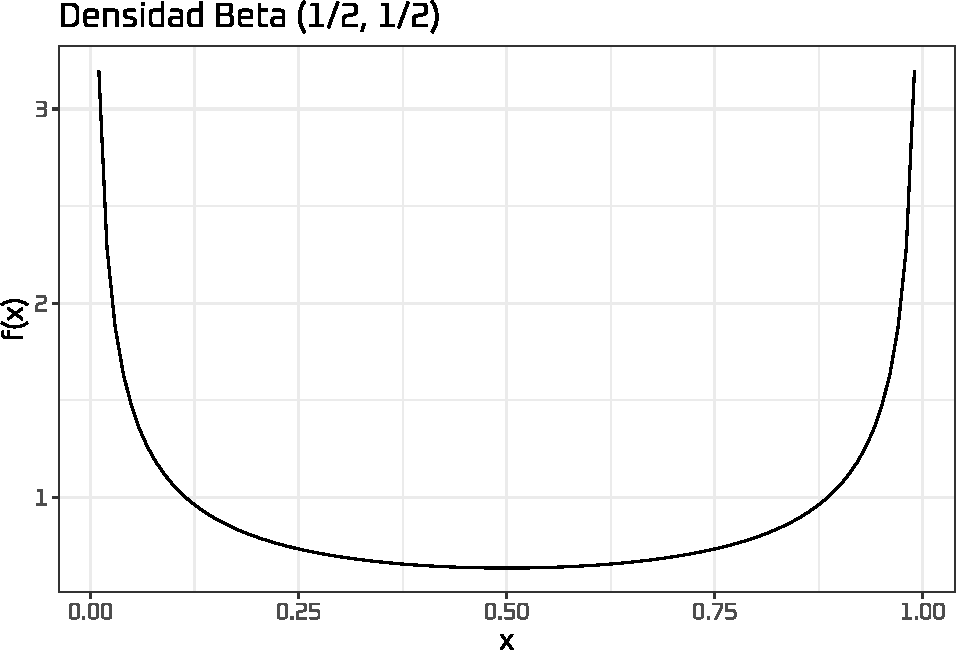
\includegraphics{3Uniparametricos_files/figure-latex/jefber1-1.pdf}
\caption{\label{fig:jefber1}Distribución previa no informativa de Jeffreys para el parámetro de una distribución Bernoulli}
\end{figure}

\begin{proposition}
\protect\hypertarget{prp:unnamed-chunk-3}{}{\label{prp:unnamed-chunk-3} }La distribución predictiva previa para una observación \(y\) está dada por
\begin{equation}
\label{eq:Predipreviabernou}
p(Y)=
\frac{Beta(y+\alpha,\beta-y+1)}{Beta(\alpha,\beta)}I_{\{0,1\}}(y)
\end{equation}
La cual define una auténtica función de densidad de probabilidad continua.
\end{proposition}

\begin{proof}
\iffalse{} {Prueba. } \fi{}De la definición de función de distribución predictiva se tiene que

\begin{align*}
p(Y)&=\int p(Y \mid \theta)p(\theta \mid \alpha,\beta)\ d\theta\\
&=\int_0^1 \theta^y(1-\theta)^{1-y}I_{\{0,1\}}(y)\frac{1}{Beta(\alpha,\beta)}\theta^{\alpha-1}(1-\theta)^{\beta-1}\ d\theta\\
&=\frac{Beta(y+\alpha,\beta-y+1)}{Beta(\alpha,\beta)}I_{\{0,1\}}(y)
    \int_0^1\frac{\theta^{y+\alpha-1}(1-\theta)^{\beta-y+1-1}}{Beta(y+\alpha,\beta-y+1)}\ d\theta\\
&=\frac{Beta(y+\alpha,\beta-y+1)}{Beta(\alpha,\beta)}I_{\{0,1\}}(y)
\end{align*}

Nótese que en la anterior expresión, la integral al lado derecho de la tercera igualdad es igual a la unidad, puesto que la expresión matemática dentro de la integral corresponde a la función de densidad de una variable aleatoria con distribucion \(Beta\), que tiene rango en el intervalo \((0,1)\). Por otro lado se deben verificar las dos condiciones de función de densidad. Es decir

\begin{enumerate}
\def\labelenumi{\arabic{enumi}.}
\tightlist
\item
  \(p(Y)>0 \ \forall y \in Y)\). Esta condición se tiene trivialmente puesto que la función matemática Beta siempre toma valores positivos.
\item
  \(\int p(y)\ dx=1\). En este caso, esta función es discreta definida en el conjunto \(\{0,1\}\). Por lo tanto esta condición es equivalente a
  \begin{equation*}
  \sum_{y\in{\{0,1\}}}P(Y=y)=
    \sum_{y\in{\{0,1\}}}\frac{Beta(y+\alpha,\beta-y+1)}{Beta(\alpha,\beta)}
  =1
  \end{equation*}
\end{enumerate}

Lo cual se verifica fácilmente teniendo en cuenta las propiedades de la función matemática Beta y de la función matemática Gamma.
\end{proof}

La distribución predictiva dada en \eqref{eq:Predipreviabernou} está
basada únicamente en la distribución previa del parámetro \(\theta\). Una
vez observada la variable \(Y\) se puede pensar en actualizar la
distribución predictiva basando la inferencia en la distribución
posterior del parámetro; esta distribución se da en el siguiente
resultado.

\begin{proposition}
\protect\hypertarget{prp:unnamed-chunk-5}{}{\label{prp:unnamed-chunk-5} }Después de la recolección de los datos, la distribución predictiva posterior para una nueva observación \(\tilde{y}\) está dada por

\begin{equation}
p(\tilde{y} \mid Y)=
  \frac{Beta(\tilde{y}+y+\alpha,\beta-\tilde{y}-y+2)}{Beta(y+\alpha,\beta-y+1)}I_{\{0,1\}}(\tilde{y}),
\end{equation}
\end{proposition}

\begin{proof}
\iffalse{} {Prueba. } \fi{}De la definición de función de distribución predictiva se tiene que

\begin{align*}
p(\tilde{y} \mid Y)&=\int p(\tilde{y} \mid \theta)p(\theta \mid Y)\ d\theta\\
&=\int_0^1\theta^{\tilde{y}}(1-\theta)^{1-\tilde{y}}I_{\{0,1\}}(\tilde{y})\frac{\theta^{y+\alpha-1}(1-\theta)^{\beta-y+1-1}}{Beta(y+\alpha,\beta-y+1)}\ d\theta\\
&=\frac{Beta(\tilde{y}+y+\alpha,\beta-\tilde{y}-y+2)}{Beta(y+\alpha,\beta-y+1)}I_{\{0,1\}}(\tilde{y})\\
&\hspace{2cm}\times \int_0^1\frac{\theta^{\tilde{y}+y+\alpha-1}(1-\theta)^{\beta-\tilde{y}-y+2-1}}{Beta(\tilde{y}+y+\alpha,\beta-\tilde{y}-y+2)}\ d\theta\\
&=\frac{Beta(\tilde{y}+y+\alpha,\beta-\tilde{y}-y+2)}{Beta(y+\alpha,\beta-y+1)}I_{\{0,1\}}(\tilde{y})
\end{align*}
\end{proof}

En la práctica rara vez se observa la realización de una única variable
aleatoria Bernoulli \(Y\), sino una muestra de variables aleatorias \(Y_1\),
\(\cdots\), \(Y_n\). En este caso, la distribución posterior del parámetro
\(\theta\) está dada en el siguiente resultado.

\begin{proposition}
\protect\hypertarget{prp:unnamed-chunk-7}{}{\label{prp:unnamed-chunk-7} }Cuando se tiene una muestra aleatoria \(Y_1,\ldots,Y_n\) de variables con distribución Bernoulli de parámetro \(\theta\), entonces la distribución posterior del parámetro de interés es

\begin{equation*}
\theta \mid Y_1,\ldots,Y_n \sim Beta\left(\sum_{i=1}^ny_i+\alpha,\beta-\sum_{i=1}^ny_i+n\right)
\end{equation*}
\end{proposition}

\begin{example}
\protect\hypertarget{exm:bernoelectoral}{}{\label{exm:bernoelectoral} }Es común en muchos países del mundo que se presenten encuestas de opinión electoral unas semanas antes de las elecciones presidenciales. Dentro de este tipo de encuestas se acostumbra a indagar acerca del favoritismo de los candidatos involucrados en la contienda electoral. Suponga que el candidato presidencial A está interesado en conocer su intención de voto previa a las elecciones. Para esto, él contrata a una firma encuestadora para la realización de una encuesta entre la población votante. El resultado de este estudio puede hacer cambiar o afirmar las estrategias publicitarias y la redefinición de la campaña electoral. La firma encuestadora decide implementar una estrategia de muestreo con un tamaño de muestra de doce mil personas. A cada respondiente se le realiza la siguiente pregunta:

\begin{quote}
Si las elecciones presidenciales fueran mañana. ¿Usted votaría por el candidato A?
\end{quote}

Las respuestas a esta pregunta son realizaciones de una muestra aleatoria de doce mil variables con densidad Bernoulli. Los resultados del estudio arrojan que 6360 personas de las personas entrevistadas, es decir un 53\%, votarían por el suscrito candidato. Técnicamente se debe analizar esta cifra puesto que las implicaciones de ganar en una primera vuelta son grandes en el sentido económico, logístico y administrativo. Claramente, el dato 53\% asegura una ventaja dentro de la muestra de doce mil personas. Sin embargo, es necesario realizar un estudio más profundo acerca de la caracterización estructural de la intención de voto del candidato en el electorado.

Con base en lo anteriormente expuesto, se decide utilizar la inferencia bayesiana puesto que existe información previa de un estudio anterior, contratado por el mismo candidato unos meses atrás en donde se entrevistaron a mil personas, con un favoritismo que estaba alrededor del 35 por ciento. Esta situación conlleva a la utilización de la metodología bayesiana que incorpora la información pasada acerca del mismo fenómeno.

El estadístico de la firma encuestadora decide utilizar una distribución previa Beta, definiendo los parámetros de la distribución previa como \(\alpha\) igual al número de votantes a favor y \(\beta\) igual al número de votantes en contra. Es decir, \(Beta(\alpha=350, \beta=650)\). Por lo anterior, la distribución posterior del parámetro de interés, que representa la probabilidad de éxito en las elecciones presidenciales, es \(Beta(6360+350, 650-6360+12000)=Beta(6710, 6290)\). Por lo tanto, utilizando la distribución posterior, se estima que la intención de voto por el candidato es de \(\frac{6710}{6710+6290}=\frac{6710}{13000}=0.516\) y este valor equivale a la media de la distribución posterior.

Sin embargo, si no se tuviese información previa como la suministrada por el estudio de meses anteriores, el análisis bayesiano sugeriría trabajar con una distribución previa no informativa, que en este caso, correspondería a una \(Beta(\alpha=0.5, \beta=0.5)\). siguiendo el mismo análisis, se tiene que la distribución posterior es \(Beta(6360.5, 5640.5)\). Finalmente, se estimaría que la intención de voto por el candidato es de \(\frac{6350.5}{12001}=0.529\).

La figuras \ref{fig:BernoEj1} muestra el comportamiento de las distribuciones previas y posteriores en ambos escenarios. Nótese que la distribución no informativa influye muy poco en el comportamiento de la distribución posterior.
\end{example}

\begin{figure}
\centering
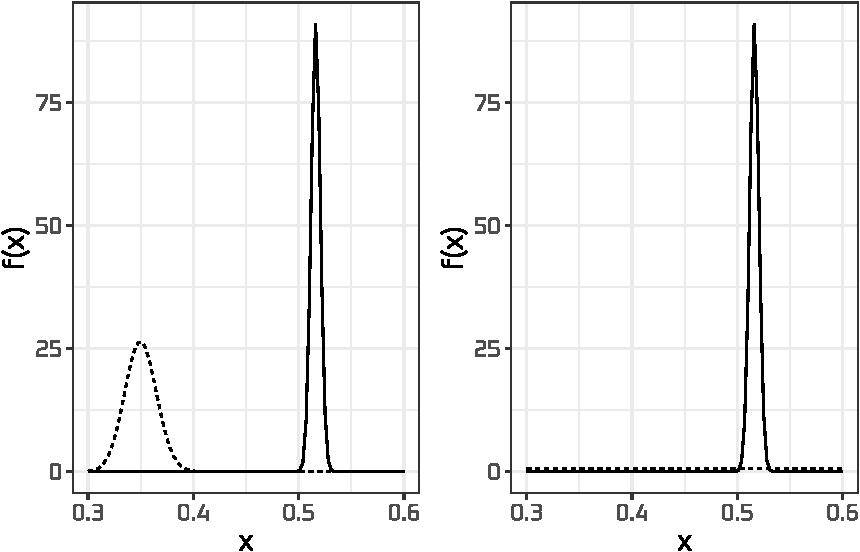
\includegraphics{3Uniparametricos_files/figure-latex/BernoEj1-1.pdf}
\caption{\label{fig:BernoEj1}Distribuciones previas (línea punteada) y posteriores (línea sólida) para el ejemplo de las encuestas electorales.}
\end{figure}

Utilizando el siguiente código en R, es posible conocer los intervalos
de credibilidad para las dos distribuciones posteriores. Además, es
posible concluir que, en ambos escenarios, el candidato aventaja
significativamente a sus contrincantes y, salvo algún cambio drástico en
el comportamiento del electorado, ganará las elecciones. Lo anterior se
deduce puesto que el intervalo de credibilidad al 95 \% no contiene
ningún valor menor a 0.5

\begin{Shaded}
\begin{Highlighting}[]
\FunctionTok{qbeta}\NormalTok{(}\FunctionTok{c}\NormalTok{(}\FloatTok{0.025}\NormalTok{, }\FloatTok{0.975}\NormalTok{), }\DecValTok{6710}\NormalTok{, }\DecValTok{6290}\NormalTok{)}
\end{Highlighting}
\end{Shaded}

\begin{verbatim}
## [1] 0.5075614 0.5247415
\end{verbatim}

\begin{Shaded}
\begin{Highlighting}[]
\FunctionTok{qbeta}\NormalTok{(}\FunctionTok{c}\NormalTok{(}\FloatTok{0.025}\NormalTok{, }\FloatTok{0.975}\NormalTok{), }\FloatTok{6350.5}\NormalTok{, }\FloatTok{5640.5}\NormalTok{)}
\end{Highlighting}
\end{Shaded}

\begin{verbatim}
## [1] 0.5206678 0.5385340
\end{verbatim}

Por otro lado, el siguiente código en \texttt{STAN} permite obtener el mismo
tipo de inferencia creando cuatro cadenas cuya distribución de
probabilidad coincide con la distribución posterior del ejemplo.

\begin{Shaded}
\begin{Highlighting}[]
\NormalTok{Bernoulli }\OtherTok{\textless{}{-}} \StringTok{"}
\StringTok{data \{}
\StringTok{  int\textless{}lower=0\textgreater{} n;}
\StringTok{  int y[n];}
\StringTok{\}}
\StringTok{parameters \{}
\StringTok{  real\textless{}lower=0, upper=1\textgreater{} theta;}
\StringTok{\}}
\StringTok{model \{}
\StringTok{  y \textasciitilde{} bernoulli(theta);}
\StringTok{  theta \textasciitilde{} beta(350, 650);}
\StringTok{\}}

\StringTok{"}

\FunctionTok{library}\NormalTok{(rstan)}
\FunctionTok{options}\NormalTok{(}\AttributeTok{mc.cores =}\NormalTok{ parallel}\SpecialCharTok{::}\FunctionTok{detectCores}\NormalTok{())}

\NormalTok{n }\OtherTok{\textless{}{-}} \DecValTok{12000}
\NormalTok{s }\OtherTok{\textless{}{-}} \DecValTok{6350}
\NormalTok{y }\OtherTok{\textless{}{-}} \FunctionTok{c}\NormalTok{(}\FunctionTok{rep}\NormalTok{(}\DecValTok{1}\NormalTok{, s), }\FunctionTok{rep}\NormalTok{(}\DecValTok{0}\NormalTok{, n }\SpecialCharTok{{-}}\NormalTok{ s))}
\NormalTok{sample\_data }\OtherTok{\textless{}{-}} \FunctionTok{list}\NormalTok{(}\AttributeTok{n =}\NormalTok{ n, }\AttributeTok{y =}\NormalTok{ y)}

\NormalTok{Berfit }\OtherTok{\textless{}{-}} \FunctionTok{stan}\NormalTok{(}\AttributeTok{model\_code =}\NormalTok{ Bernoulli, }
               \AttributeTok{data =}\NormalTok{ sample\_data, }\AttributeTok{verbose =} \ConstantTok{FALSE}\NormalTok{)}
\end{Highlighting}
\end{Shaded}

La siguiente salida de \texttt{STAN} permite conocer la estimación bayesiana posterior y los límites del intervalo de credibilidad al 95\%.

\begin{Shaded}
\begin{Highlighting}[]
\FunctionTok{print}\NormalTok{(Berfit, }\AttributeTok{pars =} \StringTok{"theta"}\NormalTok{, }
      \AttributeTok{digits =} \DecValTok{4}\NormalTok{, }\AttributeTok{probs =} \FunctionTok{c}\NormalTok{(}\FloatTok{0.025}\NormalTok{, }\FloatTok{0.975}\NormalTok{))}
\end{Highlighting}
\end{Shaded}

\begin{verbatim}
## Inference for Stan model: 62d7c91114fcc6227deb68f6059b2b09.
## 4 chains, each with iter=2000; warmup=1000; thin=1; 
## post-warmup draws per chain=1000, total post-warmup draws=4000.
## 
##         mean se_mean     sd   2.5% 97.5% n_eff   Rhat
## theta 0.5155   1e-04 0.0042 0.5071 0.524  1591 1.0009
## 
## Samples were drawn using NUTS(diag_e) at Sat Jun  5 00:10:46 2021.
## For each parameter, n_eff is a crude measure of effective sample size,
## and Rhat is the potential scale reduction factor on split chains (at 
## convergence, Rhat=1).
\end{verbatim}

\hypertarget{modelo-binomial}{%
\section{Modelo Binomial}\label{modelo-binomial}}

Cuando se dispone de una muestra aleatoria de variables con distribución
Bernoulli \(Y_1,\ldots,Y_n\), la inferencia bayesiana se puede llevar a
cabo usando la distribución Binomial, puesto que es bien sabido que la
suma de variables aleatorias Bernoulli

\begin{equation*}
S=\sum_{i=1}^nY_i
\end{equation*}

sigue una distribución Binomial. Es decir:

\begin{equation}
p(S \mid \theta)=\binom{n}{s}\theta^s(1-\theta)^{n-s}I_{\{0,1,\ldots,n\}}(s),
\end{equation}

Nótese que la distribución binomial es un caso general para la
distribución Bernoulli, cuando \(n=1\). Entonces, así como en la
distribución Bernoulli, el parámetro \(\theta\) está restringido al
espacio \(\Theta=[0,1]\). Luego, es admisible proponer que \(\theta\) siga
una distribución Beta. Por tanto la distribución previa del parámetro
\(\theta\) está dada por la expresión \eqref{eq:betadistribution}. Bajo
este marco de referencia se tienen los siguientes resultados

\begin{proposition}
\protect\hypertarget{prp:unnamed-chunk-11}{}{\label{prp:unnamed-chunk-11} }La distribución posterior del parámetro \(\theta\) sigue una distribución

\begin{equation*}
\theta \mid S \sim Beta(s+\alpha,\beta-s+n)
\end{equation*}
\end{proposition}

\begin{proof}
\iffalse{} {Prueba. } \fi{}\begin{align*}
p(\theta \mid S)&\propto p(S \mid \theta)p(\theta \mid \alpha,\beta)\\
&=\frac{\binom{n}{s}I_{\{0,1,\ldots,n\}}(s)}{Beta(\alpha,\beta)}
\theta^s\theta^{\alpha-1} (1-\theta)^{\beta-1}(1-\theta)^{n-s}I_{[0,1]}(\theta)\\
&\propto \theta^{s+\alpha-1} (1-\theta)^{\beta-s+n-1}I_{[0,1]}(\theta)
\end{align*}

Por lo tanto, factorizando convenientemente, se llega a una expresión idéntica a la función de distribución de una variable aleatoria con distribución \(Beta(s+\alpha,\beta-s+n)\).
\end{proof}

Del resultado anterior podemos ver que el estimador bayesiano de
\(\theta\) está dada por la esperanza de la distribución posterior, dada
por

\begin{equation}
\label{eq:estibeta}
\hat{\theta}_{B}=\frac{s+\alpha}{n+\alpha+\beta}
\end{equation}

En la práctica, se acostumbra a escoger los hiperparámetros \(\alpha\) y
\(\beta\) de tal forma que correspondan respectivamente al número de
éxitos y fracasos obtenidos en datos que pudieron ser recolectados
previamente. De esta forma, \(\hat{\theta}_{P}=\alpha/(\alpha+\beta)\)
corresponde a la estimación previa del parámetro \(\theta\). Por otro
lado, el estimador clásico de \(\theta\) está dado por
\(\hat{\theta}_{C}=s/n\). Entonces es posible notar que el estimador
bayesiano de \(\theta\) en \eqref{eq:estibeta} de alguna forma combina el
estimador clásico con el estimador previo. Más aún, se puede ver que
\(\hat{\theta}_{B}\) se puede escribir como un promedio ponderado entre la
estimación clásica y la estimación previa. Puesto que

\begin{align*}
\hat{\theta}_{B}=\frac{s+\alpha}{n+\alpha+\beta}&=\frac{s}{n+\alpha+\beta}+\frac{\alpha}{n+\alpha+\beta}\\
&=\frac{n}{n+\alpha+\beta}\frac{s}{n}+\frac{\alpha+\beta}{n+\alpha+\beta}\frac{\alpha}{\alpha+\beta}\\
&=\frac{n}{n+\alpha+\beta}\hat{\theta}_{C}+\frac{\alpha+\beta}{n+\alpha+\beta}\hat{\theta}_{P}
\end{align*}

De esta forma, queda en evidencia que la estimación bayesiana de
\(\theta\) siempre será un valor intermedio entre la estimación clásica y
la estimación previa. La figura \ref{fig:beta3} da una ilustración
acerca de la anterior afirmación, en donde se puede observar que para
una distribución previa concentrada en \(2/7\) y una función de
verosimilitud\footnote{La función de verosimilitud es una función del parámetro
  y sólo se puede graficar una vez se hayan observado las realizaciones de
  la variable aleatoria.} con máximo en \(8/10\), entonces la distribución
posterior estará centrada en \(10/17\); es decir, la estimación bayesiana
se encuentra situada entre la estimación previa y la estimación clásica.

\begin{figure}
\centering
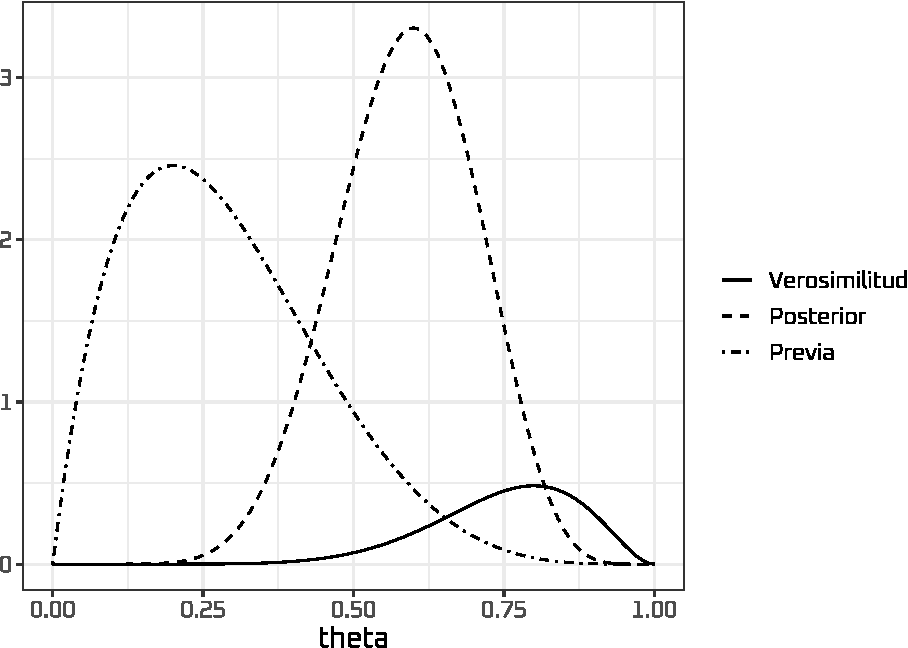
\includegraphics{3Uniparametricos_files/figure-latex/beta3-1.pdf}
\caption{\label{fig:beta3}Funciones de verosimilitud, previa y posterior para \(\alpha=2\), \(\beta=5\), \(s=8\) y \(n=10\).}
\end{figure}

Por otro lado, entre más grande sea el tamaño muestral \(n\), más
cercano estará \(\hat{\theta}_{B}\) de \(\hat{\theta}_{C}\) o
equivalentemente la función de densidad posterior de \(\theta\) estará más
concentrada en \(s/n\); mientras que entre mayor número de datos tenga la
muestra de la distribución previa (\(\alpha+\beta\) = número de datos), más
cercano estará \(\hat{\theta}_{B}\) de \(\hat{\theta}_{P}\) y la densidad
posterior de \(\theta\) estará más concentrada en \(\alpha/(\alpha+\beta)\).

Para ilustrar lo anterior, suponga que la distribución previa de
\(\theta\) está parametrizada con \(\alpha=\beta=5\), es decir la estimacion previa es 0.5, y suponga además que la estimación clásica es 0.33, pero el tamaño muestral \(n\) incrementa manteniendo constante la estimacion
clásica. En la figura \ref{fig:betan} se muestra la estimación posterior de
\(\theta\), es evidente que a medida que el tamaño muestral \(n\) aumenta,
la estimación posterior se acerca más a la estimación clásica.

\begin{figure}
\centering
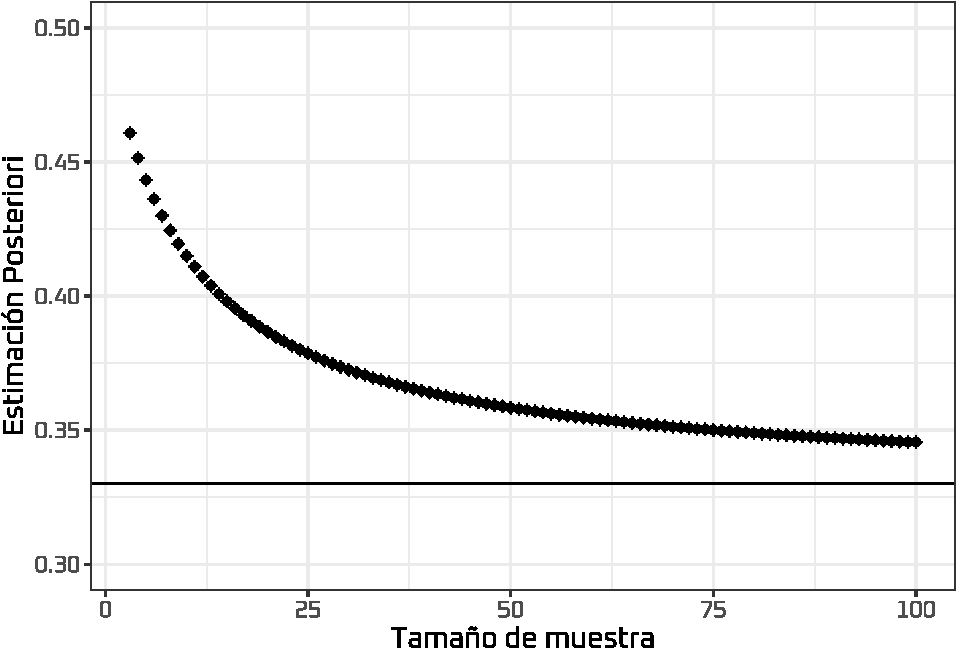
\includegraphics{3Uniparametricos_files/figure-latex/betan-1.pdf}
\caption{\label{fig:betan}Estimación posterior de \(\theta\) para diferentes valores de \(n\) y \(s\) con \(\alpha=\beta=5\).}
\end{figure}

Anteriormente, se comentó que se acostumbra a escoger los parámetros
\(\alpha\) y \(\beta\) que correspondan al número de éxitos y fracasos en la
información previa. Sin embargo, la información previa puede no
presentarse de esta forma. Por ejemplo, en algunas situaciones, la
información previa puede proveer el valor de \(\theta\), es decir, el
valor de \(\hat{\theta}_P\), y el valor de la desviación estándar de la
estimación (comúnmente conocido como el error estándar). Por ejemplo,
suponga que \(\hat{\theta}_P=0.5\) con un error estándar de 0.1, entonces
podemos encontrar los valores de \(\alpha\) y \(\beta\) de las expresiones
\(\frac{\alpha}{\alpha+\beta}=0.5\) y
\(\sqrt{\frac{\alpha\beta}{(\alpha+\beta)^2(\alpha+\beta+1)}}=0.1\), de
donde se tiene que \(\alpha=12\) y \(\beta=12\), y la distribución previa
correspondiente \(Beta(12, 12)\) tiene una esperanza de 0.05 y una
desviación estándar de 0.1. Se puede ver que entre mayor sea la
desviación estándar, menores resultan los valores de \(\alpha\) y \(\beta\),
que conducen a una distribución previa menos informativa.

Ahora, se vio anteriomente que la distribución previa no informativa de
Jeffreys corresponde a la distribución \(Beta(1/2, 1/2)\), la cual conduce
a la distribución posterior \(Beta(s+1/2, n-s+1/2)\), que a su vez nos
lleva al estimador

\begin{equation}
\label{eq:EstithetaJeffreys}
\hat{\theta}_B=\frac{s+1/2}{n+1}
\end{equation}

La anterior expresión es comparable con el estimador clásico
\(\hat{\theta}_C=\frac{s}{n}\), en el sentido de que los dos son
aplicables cuando no se dispone de ninguna información previa. Podemos
observar que, aparte del alto grado de similitud que tienen los dos
estimadores, es preferible usar el estimador \eqref{eq:EstithetaJeffreys} en situaciones donde el valor teórico de \(\theta\) es muy pequeño, y
como consecuencia \(s=0\) en la muestra. Por ejemplo, cuando \(\theta\)
representa el porcentaje de personas que están infectados con algún
virus poco común. En estos casos, el estimador clásico
\(\hat{\theta}_C=0\) sugiriendo que ningún porcentaje de la población está
infectado, conclusión que puede ser errónea. Por otro lado, el estimador
bayesiano \(\hat{\theta}_B=\frac{0.5}{n+1}\) tiende a un porcentaje muy pequeño a medida que aumente el tamaño muestral \(n\),
pero nunca llega a ser nulo.

En el siguiente resultado, se encuentra la distribución predictiva
previa para una variable binomial \(S\).

\begin{proposition}
\protect\hypertarget{prp:unnamed-chunk-13}{}{\label{prp:unnamed-chunk-13} }La distribución predictiva previa para la observación particular de la suma de variables aleatorias Bernoulli, \(s\), está dada por una distribución Beta-Binomial

\begin{equation}
p(S)=\binom{n}{s}\frac{Beta(s+\alpha,\beta-s+n)}{Beta(\alpha,\beta)}I_{\{0,1,\ldots,n\}}(s)
\end{equation}
\end{proposition}

\begin{proof}
\iffalse{} {Prueba. } \fi{}De la definición de función de distribución predictiva previa se tiene que

\begin{align*}
p(S)
&=\int p(S \mid \theta)p(\theta \mid \alpha,\beta)\ d\theta\\
&=\int_0^1\binom{n}{s}\theta^s(1-\theta)^{n-s}I_{\{0,1,\ldots,n\}}(s)
\frac{1}{Beta(\alpha,\beta)}\theta^{\alpha-1}(1-\theta)^{\beta-1}\ d\theta\\
&=\binom{n}{s}\frac{Beta(s+\alpha,\beta-s+n)}{Beta(\alpha,\beta)}I_{\{0,1,\ldots,n\}}(s)\\
&\hspace{2cm}\times\int_0^1\frac{\theta^{s+\alpha-1}(1-\theta)^{\beta-s+n-1}}{Beta(s+\alpha,\beta-s+n)}\ d\theta\\
&=\binom{n}{s}\frac{Beta(s+\alpha,\beta-s+n)}{Beta(\alpha,\beta)}I_{\{0,1,\ldots,n\}}(s)
\end{align*}
\end{proof}

Una vez observados los valores muestrales, podemos encontrar la
distribución predictiva posterior para una nueva variable binomial
\(\tilde{S}\) en una muestra de tamaño \(\tilde{n}\). Esta distribución se
encuentra en el siguiente resultado.

\begin{proposition}
\protect\hypertarget{prp:ResPredBinom}{}{\label{prp:ResPredBinom} }Después de la recolección de los datos \(y_1\), \(\cdots\), \(y_n\), la distribución predictiva posterior para una nueva variable \(\tilde{S}\) en una muestra del tamaño \(\tilde{n}\) está dada por

\begin{equation}
\label{eq:Binompredict}
p(\tilde{s} \mid S)=\binom{\tilde{n}}{\tilde{s}}\frac{Beta(\tilde{s}+s+\alpha,\beta-\tilde{s}-s+n+\tilde{n})}{Beta(s+\alpha,\beta-s+n)}I_{\{0,1,\ldots,\tilde{n}\}}(\tilde{s}),
\end{equation}
\end{proposition}

\begin{proof}
\iffalse{} {Prueba. } \fi{}De la definición de función de distribución predictiva se tiene que

\begin{align*}
p(\tilde{s} \mid S)&=\int p(\tilde{s} \mid \theta)p(\theta \mid S)\ d\theta\\
&=\int_0^1 \binom{\tilde{n}}{\tilde{s}} \theta^{\tilde{s}}(1-\theta)^{\tilde{n}-\tilde{s}}I_{\{0,1,\ldots,\tilde{n}\}}(\tilde{s})
\frac{\theta^{s+\alpha-1}(1-\theta)^{\beta-s+n-1}}{Beta(s+\alpha,\beta-s+n)}\ d\theta\\
&=\binom{\tilde{n}}{\tilde{s}}\frac{Beta(\tilde{s}+s+\alpha,\beta-\tilde{s}-s+n+\tilde{n})}{Beta(s+\alpha,\beta-s+n)}I_{\{0,1,\ldots,\tilde{n}\}}(\tilde{s})\\
& \hspace{2cm}\times
\int_0^1\frac{\theta^{\tilde{s}+s+\alpha-1}(1-\theta)^{\beta-\tilde{s}-s+n+\tilde{n}-1}}
{Beta(\tilde{s}+s+\alpha,\beta-\tilde{s}-s+n+\tilde{n})}\ d\theta\\
&=\binom{\tilde{n}}{\tilde{s}}\frac{Beta(\tilde{s}+s+\alpha,\beta-\tilde{s}-s+n+\tilde{n})}{Beta(s+\alpha,\beta-s+n)}I_{\{0,1,\ldots,\tilde{n}\}}(\tilde{s})
\end{align*}
\end{proof}

En la anterior distribución predictiva, se necesita calcular funciones
Beta. Cuando los tamaños muestrales \(n\), \(\tilde{n}\) y/o los
parámetros de la distribución previa \(\alpha\) y \(\beta\) son muy grandes,
\texttt{R} puede presentar problemas numéricos al momento de calcular directamente estas funciones. Por ejemplo, supongamos que \(n=1000\), \(s=650\), \(\alpha=200\), \(\beta=300\) y \(\tilde{n}=800\), de esta forma, los posibles
valores para \(\tilde{s}\) son \(0,1,\cdots,800\), y se tiene que la
probabilidad de que \(\tilde{s}\) tome el valor 500 está dada por

\begin{equation}
\label{eq:Ejebinom}
Pr(\tilde{s}=500|S)=
\binom{800}{500}\frac{Beta(1350,950)}{Beta(850,650)}
\end{equation}

y desafortunadamente, en \textsf{R} se presenta error al intentar
ejecutar \texttt{beta(1350,950)} o \texttt{beta(850,650)}.

\begin{Shaded}
\begin{Highlighting}[]
\FunctionTok{beta}\NormalTok{(}\DecValTok{1350}\NormalTok{, }\DecValTok{950}\NormalTok{)}
\end{Highlighting}
\end{Shaded}

\begin{verbatim}
## [1] 0
\end{verbatim}

\begin{Shaded}
\begin{Highlighting}[]
\FunctionTok{beta}\NormalTok{(}\DecValTok{850}\NormalTok{, }\DecValTok{650}\NormalTok{)}
\end{Highlighting}
\end{Shaded}

\begin{verbatim}
## [1] 0
\end{verbatim}

Por ende, es posible plantear la
siguiente solución numérica cuando se quiere calcular la función
predictiva \eqref{eq:Binompredict} en muestras grandes. El problema
central es el cómputo de \(\frac{Beta(a,b)}{Beta(c,d)}\) con \(a \geq c\) y
\(b \geq d\), valores enteros. Podemos ver que

\begin{align*}
&\ \ \ \ \frac{Beta(a,b)}{Beta(c,d)}\\
&=\frac{(a-1)!(b-1)!(c+d-1)!}{(c-1)!(d-1)!(a+b-1)!}\\
&=\frac{(a-1)(a-2)\cdots(a-(a-c))(b-1)(b-2)\cdots(b-(b-d))}{(a+b-1)(a+b-2)\cdots(a+b-(a+b-c-d))}\\
&=\frac{a^{a-c}(1-\frac{1}{a})(1-\frac{2}{a})\cdots(1-\frac{a-c}{a})b^{b-d}(1-\frac{1}{b})(1-\frac{2}{b})\cdots(1-\frac{b-d}{b})}{(a+b)^{a+b-c-d}(1-\frac{1}{a+b})(1-\frac{2}{a+b})\cdots(1-\frac{a+b-c-d}{a+b})}\\
&=\underbrace{\left(\frac{a}{a+b}\right)^{a-c}}_{t_1}\underbrace{\left(\frac{b}{a+b}\right)^{b-d}}_{t_2}\underbrace{(1-\frac{1}{a})(1-\frac{2}{a})\cdots(1-\frac{a-c}{a})}_{t_3}\\
&\ \ \ \ \ \ \underbrace{(1-\frac{1}{b})(1-\frac{2}{b})\cdots(1-\frac{b-d}{b})}_{t_4}\underbrace{(1-\frac{1}{a+b})(1-\frac{2}{a+b})\cdots(1-\frac{a+b-c-d}{a+b})}_{t_5}
\end{align*}

Calculando separadamente los términos \(t_1\), \(t_2\), \(t_3\), \(t_4\) y \(t_5\)
podemos calcular \(\frac{Beta(a,b)}{Beta(c,d)}\) para valores grandes de
\(a\), \(b\), \(c\) y \(d\). La siguiente función \texttt{prob} calcula la
densidad \eqref{eq:Binompredict} para un valor particular de \(\tilde{s}\)
usando la anterior técnica.

\begin{Shaded}
\begin{Highlighting}[]
\NormalTok{prob }\OtherTok{\textless{}{-}} \ControlFlowTok{function}\NormalTok{(s.mono, n.mono, s, n, alfa, beta)\{}
\NormalTok{  a }\OtherTok{\textless{}{-}}\NormalTok{ s.mono }\SpecialCharTok{+}\NormalTok{ s }\SpecialCharTok{+}\NormalTok{ alfa}
\NormalTok{  b }\OtherTok{\textless{}{-}}\NormalTok{ n.mono }\SpecialCharTok{{-}}\NormalTok{ s.mono }\SpecialCharTok{+}\NormalTok{ n }\SpecialCharTok{{-}}\NormalTok{ s }\SpecialCharTok{+}\NormalTok{ beta }
\NormalTok{  c }\OtherTok{\textless{}{-}}\NormalTok{ s }\SpecialCharTok{+}\NormalTok{ alfa}
\NormalTok{  d }\OtherTok{\textless{}{-}}\NormalTok{ n }\SpecialCharTok{{-}}\NormalTok{ s }\SpecialCharTok{+}\NormalTok{ beta}
\NormalTok{  t1 }\OtherTok{\textless{}{-}}\NormalTok{ (a}\SpecialCharTok{/}\NormalTok{(a }\SpecialCharTok{+}\NormalTok{ b))}\SpecialCharTok{\^{}}\NormalTok{(a }\SpecialCharTok{{-}}\NormalTok{ c)}
\NormalTok{  t2 }\OtherTok{\textless{}{-}}\NormalTok{ (b}\SpecialCharTok{/}\NormalTok{(a }\SpecialCharTok{+}\NormalTok{ b))}\SpecialCharTok{\^{}}\NormalTok{(b }\SpecialCharTok{{-}}\NormalTok{ d) }
\NormalTok{  t3 }\OtherTok{\textless{}{-}} \FunctionTok{prod}\NormalTok{(}\DecValTok{1} \SpecialCharTok{{-}} \FunctionTok{c}\NormalTok{(}\DecValTok{1}\SpecialCharTok{:}\NormalTok{(a }\SpecialCharTok{{-}}\NormalTok{ c))}\SpecialCharTok{/}\NormalTok{a)}
\NormalTok{  t4 }\OtherTok{\textless{}{-}} \FunctionTok{prod}\NormalTok{(}\DecValTok{1} \SpecialCharTok{{-}} \FunctionTok{c}\NormalTok{(}\DecValTok{1}\SpecialCharTok{:}\NormalTok{(b }\SpecialCharTok{{-}}\NormalTok{ d))}\SpecialCharTok{/}\NormalTok{b) }
\NormalTok{  t5 }\OtherTok{\textless{}{-}} \FunctionTok{prod}\NormalTok{(}\DecValTok{1} \SpecialCharTok{{-}} \FunctionTok{c}\NormalTok{(}\DecValTok{1}\SpecialCharTok{:}\NormalTok{(a }\SpecialCharTok{+}\NormalTok{ b }\SpecialCharTok{{-}}\NormalTok{ c }\SpecialCharTok{{-}}\NormalTok{ d))}\SpecialCharTok{/}\NormalTok{(a }\SpecialCharTok{+}\NormalTok{ b))}
  \ControlFlowTok{if}\NormalTok{ (a}\SpecialCharTok{==}\NormalTok{c) }
\NormalTok{    resul }\OtherTok{\textless{}{-}}\NormalTok{ t2 }\SpecialCharTok{*}\NormalTok{ t4}\SpecialCharTok{/}\NormalTok{t5 }
  \ControlFlowTok{if}\NormalTok{ (b}\SpecialCharTok{==}\NormalTok{d)}
\NormalTok{    resul }\OtherTok{\textless{}{-}}\NormalTok{ t1 }\SpecialCharTok{*}\NormalTok{ t3}\SpecialCharTok{/}\NormalTok{t5}
  \ControlFlowTok{if}\NormalTok{ (a }\SpecialCharTok{\textgreater{}}\NormalTok{ c }\SpecialCharTok{\&}\NormalTok{ b }\SpecialCharTok{\textgreater{}}\NormalTok{ d)}
\NormalTok{    resul }\OtherTok{\textless{}{-}} \FunctionTok{choose}\NormalTok{(n.mono, s.mono) }\SpecialCharTok{*}\NormalTok{ t1 }\SpecialCharTok{*}\NormalTok{ t2 }\SpecialCharTok{*}\NormalTok{ t3 }\SpecialCharTok{*}\NormalTok{ t4}\SpecialCharTok{/}\NormalTok{t5}
  \FunctionTok{return}\NormalTok{(resul) }
\NormalTok{  \}}
\end{Highlighting}
\end{Shaded}

Si queremos examinar la distribución predictiva para todos valores de la
variable \(\tilde{S}\), podemos usar los siguientes códigos

\begin{Shaded}
\begin{Highlighting}[]
\NormalTok{n }\OtherTok{\textless{}{-}} \DecValTok{1000}
\NormalTok{s }\OtherTok{\textless{}{-}} \DecValTok{650} 
\NormalTok{alfa }\OtherTok{\textless{}{-}} \DecValTok{200}
\NormalTok{beta }\OtherTok{\textless{}{-}} \DecValTok{300} 
\NormalTok{n.mono }\OtherTok{\textless{}{-}}\DecValTok{800}
\NormalTok{res }\OtherTok{\textless{}{-}} \FunctionTok{rep}\NormalTok{(}\ConstantTok{NA}\NormalTok{, (}\DecValTok{1} \SpecialCharTok{+}\NormalTok{ n.mono)) }
\ControlFlowTok{for}\NormalTok{(i }\ControlFlowTok{in} \DecValTok{1}\SpecialCharTok{:}\FunctionTok{length}\NormalTok{(res))\{}
\NormalTok{  res[i] }\OtherTok{\textless{}{-}} \FunctionTok{prob}\NormalTok{(i }\SpecialCharTok{{-}} \DecValTok{1}\NormalTok{, n.mono, s, n, alfa, beta)}
\NormalTok{\}}
\end{Highlighting}
\end{Shaded}

Y como resultado, el objeto \texttt{res} contiene las 801 probabilidades asociadas a todos los posibles valores de \(\tilde{s}\). Los resultados obtenidos con la anterior técnica son equivalentes a lo
obtenido usando la función \texttt{lbeta} que computa el logaritmo natural
de la función beta. Así, para calcular la probabilidad en
\eqref{eq:Ejebinom}, simplemente usamos el siguiente código

\begin{Shaded}
\begin{Highlighting}[]
\FunctionTok{choose}\NormalTok{(}\DecValTok{800}\NormalTok{, }\DecValTok{500}\NormalTok{) }\SpecialCharTok{*} \FunctionTok{exp}\NormalTok{(}\FunctionTok{lbeta}\NormalTok{(}\DecValTok{1350}\NormalTok{, }\DecValTok{950}\NormalTok{) }\SpecialCharTok{{-}} \FunctionTok{lbeta}\NormalTok{(}\DecValTok{850}\NormalTok{, }\DecValTok{650}\NormalTok{)) }
\end{Highlighting}
\end{Shaded}

\begin{verbatim}
## [1] 0.0005969157
\end{verbatim}

Nótese que esta probabilidad es la misma contenida en la posición 501 del objeto \texttt{res} igual a \ensuremath{5.969157\times 10^{-4}}. Finalmente, se observa que la distribución predictiva \eqref{eq:Binompredict} corresponde a una distribución
Beta-binomial con parámetros \(s+\alpha\) y \(\beta-s+n\). El paquete
\texttt{VGAM} \citep{VGAM} en \texttt{R} contiene funciones que calculan la
función de densidad, función de distribución, percentiles, además de
generar números aleatorios para la distribución Beta-binomial. Las
probabilidades puntuales de \(\tilde{s}\) se puede calcular con la función
\texttt{dbetabinom}, teniendo en cuenta que los parámetros utilizados son
\(\mu=(s+\alpha)/(n+\alpha+\beta)\) y \(\rho=1/(1+n+\alpha+\beta)\). Con el
siguiente código, podemos calcular las probabilidades para todos los
posibles valores de \(\tilde{s}\).

\begin{Shaded}
\begin{Highlighting}[]
\FunctionTok{library}\NormalTok{(VGAM) }
\NormalTok{mu }\OtherTok{\textless{}{-}}\NormalTok{ (s }\SpecialCharTok{+}\NormalTok{ alfa)}\SpecialCharTok{/}\NormalTok{(n }\SpecialCharTok{+}\NormalTok{ alfa }\SpecialCharTok{+}\NormalTok{ beta)}
\NormalTok{rho }\OtherTok{\textless{}{-}} \DecValTok{1}\SpecialCharTok{/}\NormalTok{(}\DecValTok{1} \SpecialCharTok{+}\NormalTok{ n }\SpecialCharTok{+}\NormalTok{ alfa }\SpecialCharTok{+}\NormalTok{ beta) }
\NormalTok{res2 }\OtherTok{\textless{}{-}} \FunctionTok{rep}\NormalTok{(}\ConstantTok{NA}\NormalTok{, (}\DecValTok{1} \SpecialCharTok{+}\NormalTok{ n.mono)) }
\ControlFlowTok{for}\NormalTok{(i }\ControlFlowTok{in} \DecValTok{1}\SpecialCharTok{:}\FunctionTok{length}\NormalTok{(res2))\{}
\NormalTok{  res2[i] }\OtherTok{\textless{}{-}} \FunctionTok{dbetabinom}\NormalTok{(i }\SpecialCharTok{{-}} \DecValTok{1}\NormalTok{,}
                        \AttributeTok{size =}\NormalTok{ n.mono,}
                        \AttributeTok{prob =}\NormalTok{ mu,}
                        \AttributeTok{rho =}\NormalTok{ rho)}
\NormalTok{\}}
\end{Highlighting}
\end{Shaded}

Podemos observar que la posición 501 del objeto \texttt{res2} es igual a \ensuremath{5.969157\times 10^{-4}}, el cual es idéntico a lo obtenido en \texttt{res}. Adicionalmente, al escribir la distribución predictiva de
\eqref{eq:Binompredict} como la función de densidad de una distribución
Beta-binomial, se puede encontrar la esperanza de esta distribución, la
cual está dada por

\begin{equation*}
E(\tilde{S}|S)=\tilde{n}\frac{s+\alpha}{n+\alpha+\beta}
\end{equation*}

Nótese que la esperanza en la anterior expresión corresponde simplemente
al tamaño \(\tilde{n}\) de la nueva muestra multiplicado por la
estimación bayesiana del parámetro \(\theta\). Adicionalmente, la
esperanza de \(\tilde{S}\) también se puede obtener multiplicando todos los
posibles valores de \(\tilde{S}\) con su respectiva probabilidad, y sumando
al final, como se muestra a continuación.

\begin{Shaded}
\begin{Highlighting}[]
\FunctionTok{sum}\NormalTok{(res }\SpecialCharTok{*} \FunctionTok{c}\NormalTok{(}\DecValTok{0}\SpecialCharTok{:}\NormalTok{n.mono)) }
\end{Highlighting}
\end{Shaded}

\begin{verbatim}
## [1] 453.3333
\end{verbatim}

\begin{Shaded}
\begin{Highlighting}[]
\NormalTok{n.mono }\SpecialCharTok{*}\NormalTok{ (s }\SpecialCharTok{+}\NormalTok{ alfa)}\SpecialCharTok{/}\NormalTok{(n }\SpecialCharTok{+}\NormalTok{ alfa }\SpecialCharTok{+}\NormalTok{ beta)}
\end{Highlighting}
\end{Shaded}

\begin{verbatim}
## [1] 453.3333
\end{verbatim}

Retomando el ejemplo \ref{exm:bernoelectoral}, suponga que la encuesta de opinión electoral
se lleva a cabo en diferentes ciudades de un determinado país, en este
caso, para cada ciudad se tiene una muestra de variables con
distribución Bernoulli o equivalentemente una variable binomial; de esta
forma, se dispone de una muestra de variables con distribución Binomial.
La distribución posterior del parámetro \(\theta\) para estos casos se
encuentra en el siguiente resultado.

\begin{proposition}
\protect\hypertarget{prp:postbinom}{}{\label{prp:postbinom} }Cuando se tiene una sucesión de variables aleatorias \(S_1,\ldots,S_i, \ldots,S_k\) independientes y con distribución \(Binomial(n_i,\theta)\) para \(i=1,\ldots,k\), entonces la distribución posterior del parámetro de interés \(\theta\) es

\begin{equation*}
\theta \mid S_1,\ldots,S_k \sim Beta\left(\sum_{i=1}^ks_i+\alpha,\beta+\sum_{i=1}^k n_i-\sum_{i=1}^k s_i\right)
\end{equation*}
\end{proposition}

\begin{proof}
\iffalse{} {Prueba. } \fi{}\begin{align*}
p(\theta \mid S_1,\ldots,S_k)&\propto \prod_{i=1}^kp(S_i \mid \theta)p(\theta \mid \alpha,\beta)\\
&\propto \prod_{i=1}^k\theta^{\sum_{i=1}s_i}\theta^{\alpha-1}(1-\theta)^{\beta-1}
(1-\theta)^{\sum_{i=1}^kn_i-\sum_{i=1}^ks_i}I_{[0,1]}(\theta)\\
&= \theta^{\sum_{i=1}^ks_i+\alpha-1}(1-\theta)^{\sum_{i=1}^kn_i-\sum_{i=1}^ks_i+\beta}I_{[0,1]}(\theta)
\end{align*}

Por lo tanto, factorizando convenientemente, se encuentra una expresión idéntica a la función de densidad de la distribución \(Beta\left(\sum_{i=1}^ks_i+\alpha,\beta+\sum_{i=1}^k n_i-\sum_{i=1}^n s_i\right)\).
\end{proof}

\begin{example}
\protect\hypertarget{exm:unnamed-chunk-23}{}{\label{exm:unnamed-chunk-23} }El siguiente conjunto de datos fue estudiado inicialmente por \citet{Efron75} y se ha convertido en uno de los ejemplos prácticos más citados en la historia de la estadística moderna. Se trata de los porcentajes de bateo en una muestra de 18 jugadores profesionales en la temporada regular de béisbol en Estados Unidos en el año 1970. \citet{wikiBat} establece que, en términos generales, este valor representa la razón entre la cantidad de \emph{hits} y el número de turnos al bate\footnote{Un \emph{hit} es la conexión efectuada por el bateador que coloca la pelota dentro del terreno de juego, permitiéndole alcanzar al menos una base, sin que se produzca un error de defensa del equipo contrario. Para lograr un hit, el bateador debe llegar a primera base antes de que ningún jugador defensivo lo toque con la bola en el trayecto del home a la inicial, o que el jugador de la defensa que tenga la bola pise la primera base antes que el bateador llegue a la misma.}. La fórmula para calcular esta estadística es \(s/n\), donde \(s\) es el número de \emph{hits} y \(n\) es el total de turnos. Este conjunto de datos está disponible en el paquete \texttt{pscl} de \texttt{R} y se puede cargar mediante el siguiente código computacional.
\end{example}

\begin{Shaded}
\begin{Highlighting}[]
\FunctionTok{library}\NormalTok{(pscl)}
\FunctionTok{data}\NormalTok{(EfronMorris)}
\end{Highlighting}
\end{Shaded}

\begin{tabular}{l|l|l|r|r|r|r}
\hline
name & team & league & r & y & n & p\\
\hline
Roberto Clemente & Pitts & NL & 18 & 0.400 & 367 & 0.346\\
\hline
Frank Robinson & Balt & AL & 17 & 0.378 & 426 & 0.298\\
\hline
Frank Howard & Wash & AL & 16 & 0.356 & 521 & 0.276\\
\hline
Jay Johnstone & Cal & AL & 15 & 0.333 & 275 & 0.222\\
\hline
Ken Berry & Chi & AL & 14 & 0.311 & 418 & 0.273\\
\hline
Jim Spencer & Cal & AL & 14 & 0.311 & 466 & 0.270\\
\hline
Don Kessinger & Chi & NL & 13 & 0.289 & 586 & 0.263\\
\hline
Luis Alvarado & Bos & AL & 12 & 0.267 & 138 & 0.210\\
\hline
Ron Santo & Chi & NL & 11 & 0.244 & 510 & 0.269\\
\hline
Ron Swoboda & NY & NL & 11 & 0.244 & 200 & 0.230\\
\hline
Del Unser & Wash & AL & 10 & 0.222 & 277 & 0.264\\
\hline
Billy Williams & Chi & AL & 10 & 0.222 & 270 & 0.256\\
\hline
George Scott & Bos & AL & 10 & 0.222 & 435 & 0.303\\
\hline
Rico Petrocelli & Bos & AL & 10 & 0.222 & 538 & 0.264\\
\hline
Ellie Rodriguez & KC & AL & 10 & 0.222 & 186 & 0.226\\
\hline
Bert Campaneris & Oak & AL & 9 & 0.200 & 558 & 0.285\\
\hline
Thurman Munson & NY & AL & 8 & 0.178 & 408 & 0.316\\
\hline
Max Alvis & Mil & NL & 7 & 0.156 & 70 & 0.200\\
\hline
\end{tabular}

En la primera columna se tiene el número del jugador, la segunda columna proporciona el nombre del jugador, la cuarta columna representan el número de \emph{hits} en los primeros 45 turnos al bate. La sexta columna representa el número de turnos al bate al final de la temporada regular y la última columna representa el promedio de bateo en la temporada.

Suponga que, partiendo de la muestra de los 18 jugadores, el objetivo es estimar el porcentaje de bateo, notado como \(\theta\), en toda la liga en el año de 1970. En primera instancia es plausible considerar que cada uno de los jugadores se comporta de manera independiente y que el porcentaje de bateo es común a todos, puesto que pertenecen a la misma liga profesional. Por lo tanto, es posible establecer que el número de \emph{hits} \(s_i\) (\(i=1,\ldots,18\)) para cada jugador tiene la siguiente distribución

\begin{equation*}
S_i\sim Binomial (n_i,\theta) \ \ \ \ \ \ \ \ \ i=1,\ldots,18.
\end{equation*}

Utilizando un enfoque bayesiano, es posible sacar provecho de la información recolectada al principio de la temporada, constituida por la tercera y cuarta columna del archivo de datos. En esta instancia, se tuvieron \(18+17+\cdots+8+7=215\) hits para un total de \(45\times 18= 810\) turnos al bate. Con esta información, se define la caracterización estructural de la distribución previa que, siguiendo las recomendaciones anteriores, está dada por una \(Beta(\alpha=215, \beta=810-215)=Beta(\alpha=215, \beta=595)\). Del resultado \ref{prp:postbinom}, y teniendo en cuenta que al final de la temporada se obtuvieron \(\sum S_i = 1825\) \emph{hits} para un total de \(\sum n_i =6649\) turnos al bate, se tiene que la distribución posterior para este ejemplo es una \(Beta(1825+215,6649-1825+595)=Beta(2040, 5419)\). Por lo tanto, utilizando la distribución posterior, se estima que el porcentaje de bateo en la liga profesional en el año de 1970 es de \(\frac{2040}{2040+5419}=\frac{2040}{7459}=0.273\). Este valor corresponde a la media de la distribución posterior.

Nótese que los mismos resultados se encuentran cuando se analiza este conjunto de datos en \texttt{STAN}, mediante el siguiente código computacional.

\begin{Shaded}
\begin{Highlighting}[]
\NormalTok{Binomial }\OtherTok{\textless{}{-}} \StringTok{\textquotesingle{}data \{}
\StringTok{  int\textless{}lower=0\textgreater{} n;}
\StringTok{  int\textless{}lower=0\textgreater{} m[n];}
\StringTok{  int\textless{}lower=0\textgreater{} s[n];}
\StringTok{\}}
\StringTok{parameters \{}
\StringTok{  real\textless{}lower=0, upper=1\textgreater{} theta;}
\StringTok{\}}
\StringTok{model \{}
\StringTok{  for(i in 1:n) \{}
\StringTok{  s[i] \textasciitilde{} binomial(m[i], theta);}
\StringTok{  \}}
\StringTok{  theta \textasciitilde{} beta(215, 595);}
\StringTok{\}}
\StringTok{\textquotesingle{}}

\FunctionTok{library}\NormalTok{(rstan)}
\FunctionTok{options}\NormalTok{(}\AttributeTok{mc.cores =}\NormalTok{ parallel}\SpecialCharTok{::}\FunctionTok{detectCores}\NormalTok{())}

\NormalTok{s }\OtherTok{\textless{}{-}} \FunctionTok{round}\NormalTok{(EfronMorris}\SpecialCharTok{$}\NormalTok{n }\SpecialCharTok{*}\NormalTok{ EfronMorris}\SpecialCharTok{$}\NormalTok{p)}
\NormalTok{sample\_data }\OtherTok{\textless{}{-}} \FunctionTok{list}\NormalTok{(}\AttributeTok{s =}\NormalTok{ s, }
                    \AttributeTok{n =} \FunctionTok{nrow}\NormalTok{(EfronMorris),}
                    \AttributeTok{m =}\NormalTok{ EfronMorris}\SpecialCharTok{$}\NormalTok{n)}

\NormalTok{Binfit }\OtherTok{\textless{}{-}} \FunctionTok{stan}\NormalTok{(}\AttributeTok{model\_code =}\NormalTok{ Binomial, }
               \AttributeTok{data =}\NormalTok{ sample\_data, }\AttributeTok{verbose =} \ConstantTok{FALSE}\NormalTok{)}
\end{Highlighting}
\end{Shaded}

La siguiente salida de \texttt{STAN} permite conocer la estimación bayesiana posterior y los límites del intervalo de credibilidad al 95\%.

\begin{Shaded}
\begin{Highlighting}[]
\FunctionTok{print}\NormalTok{(Binfit, }\AttributeTok{pars =} \StringTok{"theta"}\NormalTok{, }
      \AttributeTok{digits =} \DecValTok{4}\NormalTok{, }\AttributeTok{probs =} \FunctionTok{c}\NormalTok{(}\FloatTok{0.025}\NormalTok{, }\FloatTok{0.975}\NormalTok{))}
\end{Highlighting}
\end{Shaded}

\begin{verbatim}
## Inference for Stan model: b5a37600d5b0f80332bf311eb740e4c6.
## 4 chains, each with iter=2000; warmup=1000; thin=1; 
## post-warmup draws per chain=1000, total post-warmup draws=4000.
## 
##         mean se_mean     sd  2.5%  97.5% n_eff  Rhat
## theta 0.2736   1e-04 0.0051 0.264 0.2838  1311 1.003
## 
## Samples were drawn using NUTS(diag_e) at Sat Jun  5 00:11:22 2021.
## For each parameter, n_eff is a crude measure of effective sample size,
## and Rhat is the potential scale reduction factor on split chains (at 
## convergence, Rhat=1).
\end{verbatim}

Por otro lado, el mismo intervalo de credibilidad del 95\% correspondiente se puede hallar mediante el siguiente código computacional de \texttt{R}.

\begin{Shaded}
\begin{Highlighting}[]
\FunctionTok{qbeta}\NormalTok{(}\FunctionTok{c}\NormalTok{(}\FloatTok{0.025}\NormalTok{, }\FloatTok{0.975}\NormalTok{), }\DecValTok{2040}\NormalTok{, }\DecValTok{5419}\NormalTok{)}
\end{Highlighting}
\end{Shaded}

\begin{verbatim}
## [1] 0.2634379 0.2836674
\end{verbatim}

La figura \ref{fig:BinomEj1} muestra el comportamiento de las distribuciones previa y posterior para este ejemplo. Nótese que, con un análisis frecuentista, se hubiese llegado a una estimación cercana de \(\frac{1825}{6649}=0.274\).

\begin{Shaded}
\begin{Highlighting}[]
\NormalTok{p }\OtherTok{\textless{}{-}} \FunctionTok{ggplot}\NormalTok{(}\AttributeTok{data =} \FunctionTok{data.frame}\NormalTok{(}\AttributeTok{x =} \DecValTok{0}\NormalTok{), }
            \AttributeTok{mapping =} \FunctionTok{aes}\NormalTok{(}\AttributeTok{x =}\NormalTok{ x)) }\SpecialCharTok{+} 
  \FunctionTok{ylab}\NormalTok{(}\StringTok{""}\NormalTok{) }\SpecialCharTok{+} \FunctionTok{xlab}\NormalTok{(}\FunctionTok{expression}\NormalTok{(theta))}
\NormalTok{previa }\OtherTok{\textless{}{-}} \ControlFlowTok{function}\NormalTok{(x) }\FunctionTok{dbeta}\NormalTok{(x, }\DecValTok{215}\NormalTok{, }\DecValTok{595}\NormalTok{)}
\NormalTok{posterior }\OtherTok{\textless{}{-}} \ControlFlowTok{function}\NormalTok{(x) }\FunctionTok{dbeta}\NormalTok{(x, }\DecValTok{2040}\NormalTok{, }\DecValTok{5419}\NormalTok{)}
\NormalTok{p }\SpecialCharTok{+} 
  \FunctionTok{stat\_function}\NormalTok{(}\AttributeTok{stat=}\StringTok{"function"}\NormalTok{, }\AttributeTok{fun =}\NormalTok{ previa,}
                \AttributeTok{mapping =} \FunctionTok{aes}\NormalTok{(}\AttributeTok{linetype=}\StringTok{"solid"}\NormalTok{)) }\SpecialCharTok{+}
  \FunctionTok{stat\_function}\NormalTok{(}\AttributeTok{stat=}\StringTok{"function"}\NormalTok{, }\AttributeTok{fun =}\NormalTok{ posterior, }
                \AttributeTok{mapping =} \FunctionTok{aes}\NormalTok{(}\AttributeTok{linetype=}\StringTok{"dashed"}\NormalTok{)) }\SpecialCharTok{+}
    \FunctionTok{xlim}\NormalTok{(}\FloatTok{0.2}\NormalTok{,}\FloatTok{0.35}\NormalTok{) }\SpecialCharTok{+}
    \FunctionTok{scale\_linetype\_manual}\NormalTok{(}\AttributeTok{name=}\StringTok{""}\NormalTok{, }\AttributeTok{values=}\FunctionTok{c}\NormalTok{(}\StringTok{"solid"}\NormalTok{, }\StringTok{"dashed"}\NormalTok{),}
        \AttributeTok{label=}\FunctionTok{c}\NormalTok{(}\StringTok{"Posterior"}\NormalTok{,}\StringTok{"Previa"}\NormalTok{)) }
\end{Highlighting}
\end{Shaded}

\begin{figure}
\centering
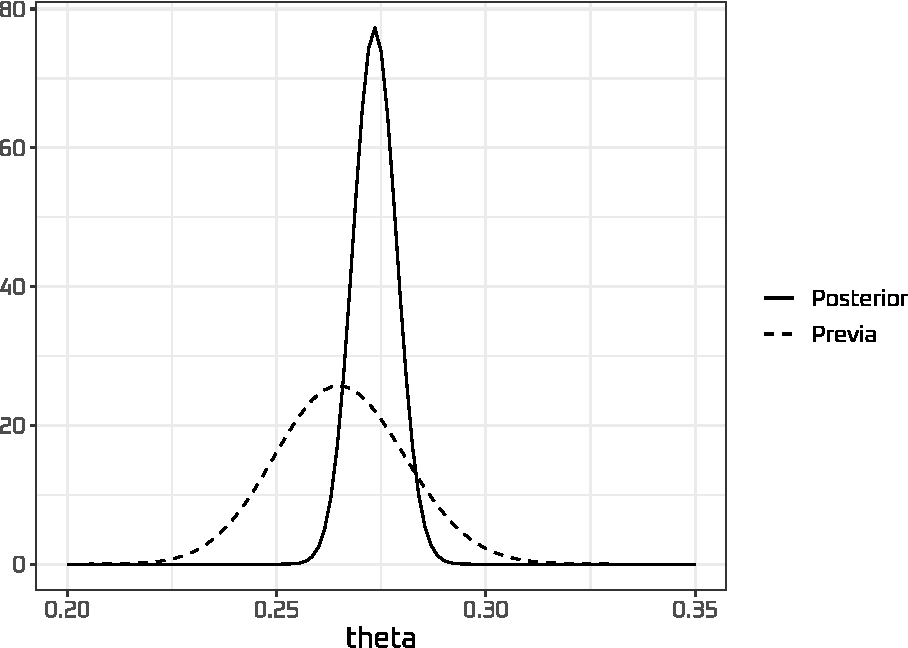
\includegraphics{3Uniparametricos_files/figure-latex/BinomEj1-1.pdf}
\caption{\label{fig:BinomEj1}Función de densidad previa y función de densidad posterior para el ejemplo de bateo.}
\end{figure}

Es posible analizar este conjunto de datos desde otra perspectiva al suponer que los jugadores no constituyen una muestra aleatoria y cada uno de ellos tiene un promedio de bateo diferente. Sin embargo, este análisis se deja como ejercicio en un capítulo posterior.

\begin{example}
\protect\hypertarget{exm:unnamed-chunk-29}{}{\label{exm:unnamed-chunk-29} }Continuando con el conjunto de datos de Efron y Morris, suponga que el entrenador de un equipo de las ligas inferiores está interesado en adquirir los servicios de Max Alvis. Este jugador no tuvo un buen promedio de bateo en la temporada y no tuvo muchos turnos al bate. El entrenador quiere conocer cuál será el número más probable de \emph{hits} que anotará en la siguiente temporada. Teniendo en cuenta que es un jugador que viene de la liga profesional, lo más conveniente es que tenga muchos turnos al bate, digamos 400.

Para resolver este cuestionamiento, es conveniente recurrir a la función predictiva posterior, dada en el resultado \ref{prp:ResPredBinom}. Para este análisis, se define la caracterización estructural de la distribución previa del jugador que está dada por una \(Beta(\alpha=7, \beta=38)\). La siguiente función en \texttt{R} permite obtener la distribución predictiva para este jugador, que se muestra en la figura \ref{fig:PredBinom}.
\end{example}

\begin{Shaded}
\begin{Highlighting}[]
\NormalTok{n }\OtherTok{\textless{}{-}} \DecValTok{70}
\NormalTok{s }\OtherTok{\textless{}{-}} \DecValTok{14}
\NormalTok{alp }\OtherTok{\textless{}{-}}\DecValTok{7}
\NormalTok{bet }\OtherTok{\textless{}{-}} \DecValTok{38}
\NormalTok{n.ast }\OtherTok{\textless{}{-}} \DecValTok{400}
\NormalTok{predictiva }\OtherTok{\textless{}{-}} \FunctionTok{rep}\NormalTok{(}\ConstantTok{NA}\NormalTok{, n.ast }\SpecialCharTok{+} \DecValTok{1}\NormalTok{)}
\ControlFlowTok{for}\NormalTok{(k }\ControlFlowTok{in} \DecValTok{0}\SpecialCharTok{:}\NormalTok{n.ast)\{}
\NormalTok{  predictiva[k }\SpecialCharTok{+} \DecValTok{1}\NormalTok{] }\OtherTok{\textless{}{-}}
  \FunctionTok{choose}\NormalTok{(n.ast,k) }\SpecialCharTok{*}
    \FunctionTok{beta}\NormalTok{(k}\SpecialCharTok{+}\NormalTok{s}\SpecialCharTok{+}\NormalTok{alp,bet}\SpecialCharTok{{-}}\NormalTok{k}\SpecialCharTok{{-}}\NormalTok{s}\SpecialCharTok{+}\NormalTok{n.ast}\SpecialCharTok{+}\NormalTok{n)}\SpecialCharTok{/}\FunctionTok{beta}\NormalTok{(s}\SpecialCharTok{+}\NormalTok{alp,bet}\SpecialCharTok{{-}}\NormalTok{s}\SpecialCharTok{+}\NormalTok{n)}
\NormalTok{\}}

\FunctionTok{sum}\NormalTok{(predictiva)}
\end{Highlighting}
\end{Shaded}

\begin{verbatim}
## [1] 1
\end{verbatim}

\begin{Shaded}
\begin{Highlighting}[]
\FunctionTok{which}\NormalTok{(predictiva}\SpecialCharTok{==}\FunctionTok{max}\NormalTok{(predictiva))}
\end{Highlighting}
\end{Shaded}

\begin{verbatim}
## [1] 71
\end{verbatim}

La última línea del código computacional permite concluir que lo más probable es que el jugador realice 71 hits en 400 turnos al bate, cifra que no convence al entrenador para adquirir los servicios del jugador.

\begin{Shaded}
\begin{Highlighting}[]
\NormalTok{predic }\OtherTok{\textless{}{-}} \FunctionTok{data.frame}\NormalTok{(}\AttributeTok{time =} \FunctionTok{c}\NormalTok{(}\DecValTok{1}\SpecialCharTok{:}\NormalTok{(n.ast }\SpecialCharTok{+} \DecValTok{1}\NormalTok{)), }
                     \AttributeTok{y =}\NormalTok{ predictiva)}
\FunctionTok{ggplot}\NormalTok{(predic, }\FunctionTok{aes}\NormalTok{(time, y)) }\SpecialCharTok{+} 
  \FunctionTok{geom\_line}\NormalTok{() }\SpecialCharTok{+} 
  \FunctionTok{xlab}\NormalTok{(}\FunctionTok{expression}\NormalTok{(}\FunctionTok{tilde}\NormalTok{(y))) }\SpecialCharTok{+} 
  \FunctionTok{ylab}\NormalTok{(}\StringTok{"Distribución posterior predictiva"}\NormalTok{)}
\end{Highlighting}
\end{Shaded}

\begin{figure}
\centering
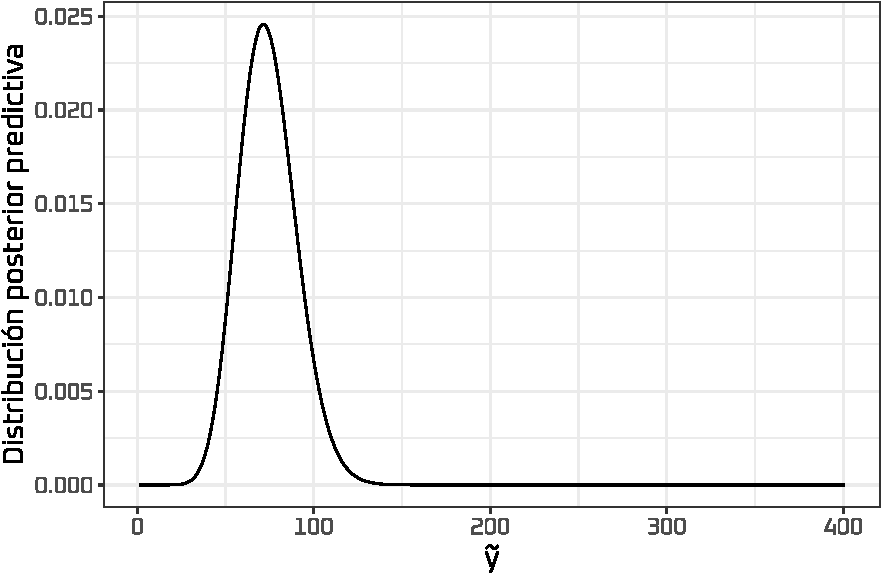
\includegraphics{3Uniparametricos_files/figure-latex/PredBinom-1.pdf}
\caption{\label{fig:PredBinom}Función de densidad predictiva posterior para el jugador Max Alvis.}
\end{figure}

\hypertarget{appendix-apuxe9ndice}{%
\appendix}


\hypertarget{elementos-de-probabilidad}{%
\chapter{Elementos de probabilidad}\label{elementos-de-probabilidad}}

ss

\hypertarget{distribuciones-discretas}{%
\section{Distribuciones discretas}\label{distribuciones-discretas}}

\hypertarget{distribuciuxf3n-uniforme-discreta}{%
\subsection{Distribución uniforme discreta}\label{distribuciuxf3n-uniforme-discreta}}

\begin{definition}
\protect\hypertarget{def:unnamed-chunk-1}{}{\label{def:unnamed-chunk-1} }Una variable aleatoria \(Y\) tiene distribución uniforme discreta sobre el conjunto \(\{1,2,\cdots,N\}\) si su función de densidad está dada por:

\begin{equation}
f_Y(y)=\frac{1}{N}I_{\{1,2,\cdots,N\}}(y)
\end{equation}
\end{definition}

Esta distribución describe situaciones donde los resultados de un experimento aleatorio tienen la misma probabilidad de ocurrencia. Entre los ejemplos de la distribución uniforme discreta en la vida práctica están el lanzamiento de una moneda corriente, el lanzamiento de un dado corriente, la extracción de una urna que contiene bolas enumeradas de 1 a \(N\).

\begin{proposition}
\protect\hypertarget{prp:unnamed-chunk-2}{}{\label{prp:unnamed-chunk-2} }Si \(Y\) es una variable aleatoria con distribución uniforme discreta sobre el conjunto \(\{1,2,\cdots,N\}\), entonces:

\begin{itemize}
\tightlist
\item
  \(E(Y)=\frac{N+1}{2}\).
\item
  \(Var(Y)=\frac{N^2-1}{12}\).
\item
  \(m_Y(t)=\sum_{i=1}^N\frac{e^{ti}}{N}\).
\end{itemize}
\end{proposition}

\hypertarget{distribuciuxf3n-hipergeomuxe9trica}{%
\subsection{Distribución hipergeométrica}\label{distribuciuxf3n-hipergeomuxe9trica}}

\begin{definition}
\protect\hypertarget{def:unnamed-chunk-3}{}{\label{def:unnamed-chunk-3} }Una variable aleatoria \(Y\) tiene distribución hipergeométrica con parámetros \(n\), \(R\) y \(N\) si su función de densidad está dada por:

\begin{equation}
f_Y(y)=\frac{\binom{R}{y}\binom{N-R}{n-y}}{\binom{N}{n}}I_{\{0,1,\cdots,n\}}(y),
\end{equation}
y se nota como \(Y\sim Hg(n,R,N)\).
\end{definition}

Suponga que en una urna hay \(N\) bolas en total, donde \(R\) de ellas son del color negro y los \(N-R\) son del color blanco, se extrae aleatoriamente
\(n\) bolas de la urna (\(n<N\)), entonces la variable ``número de bolas negras extraídas'' tiene distribución hipergeométrica con parámetros \(n\), \(R\) y
\(N\). Otro uso de la distribución hipergeométrica es el problema de captura-recaptura.

\begin{proposition}
\protect\hypertarget{prp:unnamed-chunk-4}{}{\label{prp:unnamed-chunk-4} }Si \(Y\) es una variable aleatoria con distribución hipergeométrica con parámetros \(n\), \(R\) y \(N\), entonces:

\begin{itemize}
\tightlist
\item
  \(E(Y)=\frac{nR}{N}\).
\item
  \(Var(Y)=\frac{nR(N-R)(N-n)}{N^2(N-1)}\).
\end{itemize}
\end{proposition}

El anterior resultado no incluye la función generadora de momentos, pues éste no ha resultado ser útil en la teoría relacionada con la distribución hipergeométrica.

\hypertarget{distribuciuxf3n-bernoulli}{%
\subsection{Distribución Bernoulli}\label{distribuciuxf3n-bernoulli}}

La distribución Bernoulli debe su nombre al matemático suizo Jacob Bernoulli (1654-1705) que describe el éxito o fracaso de un evento.

\begin{definition}
\protect\hypertarget{def:unnamed-chunk-5}{}{\label{def:unnamed-chunk-5} }Una variable aleatoria \(Y\) tiene distribución Bernoulli con parámetro \(p\in (0,1)\) si su función de densidad está dada por:

\begin{equation}
f_Y(y)=p^y(1-p)^{1-y}I_{\{0,1\}}(y),
\end{equation}

y se nota como \(Y\sim Ber(p)\).
\end{definition}

\begin{proposition}
\protect\hypertarget{prp:unnamed-chunk-6}{}{\label{prp:unnamed-chunk-6} }Si \(Y\) es una variable aleatoria con distribución Bernoulli con parámetro \(p\), entonces:

\begin{itemize}
\tightlist
\item
  \(E(Y)=p\).
\item
  \(Var(Y)=p(1-p)\).
\item
  \(m_Y(t)=pe^t+1-p\).
\end{itemize}
\end{proposition}

\hypertarget{distribuciuxf3n-binomial}{%
\subsection{Distribución binomial}\label{distribuciuxf3n-binomial}}

\begin{definition}
\protect\hypertarget{def:unnamed-chunk-7}{}{\label{def:unnamed-chunk-7} }Una variable aleatoria \(Y\) tiene distribución binomial con los parámetros \(n\in \mathbb{N}\) y \(p\in (0,1)\) si su función de densidad está dada por:

\begin{equation}
f_Y(y)=\binom{n}{y}p^y(1-p)^{n-y}I_{\{0,1,\cdots,n\}}(y),
\end{equation}

y se nota como \(Y\sim Bin(n,p)\).
\end{definition}

\begin{proposition}
\protect\hypertarget{prp:unnamed-chunk-8}{}{\label{prp:unnamed-chunk-8} }Sea \(Y_1\), \(\cdots\), \(Y_n\) variables aleatorias independientes e idénticamente distribuidas con distribución Bernoulli con parámetro \(p\),
entonces la variable \(\sum_{i=1}^nY_i\) tiene distribución \(Bin(n,p)\). Por ende, la distribución Bernoulli es un caso particular de la distribución binomial cuando \(n=1\).
\end{proposition}

\begin{proof}
\iffalse{} {Prueba. } \fi{}La demostración radica en el hecho de que la función generadora de momentos caracteriza la distribución probabilística, entonces basta demostrar que la función generadora de momentos de \(\sum_{i=1}^nX_i\) es la de una distribución \(Bin(n,p)\). Tenemos lo siguiente:

\begin{align*}
m_{\sum Y_i}(t)=E(e^{\sum tY_i})&=E(\prod_{i=1}^ne^{tY_i})\\
               &=\prod_{i=1}^nE(e^{tY_i})\ \ \ \ (\text{por independencia})\\
               &=\prod_{i=1}^n(pe^t+1-p)\ \ \ \ (\text{definición de $m_{Y_i}(t)$})\\
               &=(pe^t+1-p)^n
\end{align*}
\end{proof}

Una aplicación de esta distribución es cuando tenemos un número \(n\) de repeticiones independientes de un experimento donde cada uno tiene dos
posibles resultados que se podrían llamarse como éxito o fracaso y donde la probabilidad de éxito \(p\) es constante en cada una de las repeticiones. Por tanto, la variable número de éxitos obtenidos en las \(n\) repeticiones tiene distribución \(Bin(n,p)\). La distribución binomial tiene dos parámetros, \(n\) y \(p\); sin embargo, cuando \(n\) es conocido, la distribución dependerá sólo del valor \(p\) que sería el único parámetro con espacio paramétrico \(\Theta=(0,1)\).

\begin{proposition}
\protect\hypertarget{prp:unnamed-chunk-10}{}{\label{prp:unnamed-chunk-10} }Si \(Y\) es una variable aleatoria con distribución binomial con parámetros \(n\) y \(p\), entonces

\begin{itemize}
\tightlist
\item
  \(E(Y)=np\).
\item
  \(Var(Y)=np(1-p)\).
\item
  \(m_Y(t)=(pe^t+1-p)^n\).
\end{itemize}
\end{proposition}

\hypertarget{distribuciuxf3n-binomial-negativa}{%
\subsection{Distribución Binomial negativa}\label{distribuciuxf3n-binomial-negativa}}

\begin{definition}
\protect\hypertarget{def:unnamed-chunk-11}{}{\label{def:unnamed-chunk-11} }Una variable aleatoria \(Y\) tiene distribución Binomial negativa con parámetros \((\theta, r)\) si su función de densidad está dada por:

\begin{equation}
P(y\mid \theta, r)=\frac{\Gamma(r+y_i)}{y_i!\Gamma(r)}\theta^r(1-\theta)^{1-y_i}I_{(0,1,2,\ldots)}(y)
\end{equation}
\end{definition}

Esta distribución siempre ha tenido lugar al resolver el problema del número de ensayos necesarios para lograr un número específico de éxitos. Por supuesto, si \(r\) es el número de éxitos necesarios y se conoce que la probabilidad de éxito es \(\theta\), entonces la distribución binomial negativa corresponde a un modelo probabilístico, afianzado durante siglos, que permite la resolución de este tipo de situaciones.

Por otro lado, es posible asignar al parámetro \(r\) valores que sean reales; en este caso no hay ninguna interpretación práctica en el contexto del número de ensayos necesarios para determinados éxitos. Sin embargo, en términos de distribución, \(r\) es un parámetro más. Esto nos lleva a uno de los verdaderos usos prácticos de esta distribución: la sobredispersión. Dado que la forma funcional de arriba corresponde a una generalización de la función de distribución Poisson, entonces es posible suponer que los datos de conteo vienen de una distribución binomial negativa.

Lo anterior trae ventajas puesto que, si la media de los datos recolectados no corresponde con la varianza (característica esencial de la Poisson), entonces cualquier modelo que de allí surgiese sería altamente cuestionable. Si lo anterior se presenta es mejor acudir a la distribución binomial negativa dando valores reales al parámetro \(r\).

\begin{proposition}
\protect\hypertarget{prp:unnamed-chunk-12}{}{\label{prp:unnamed-chunk-12} }Si \(Y\) es una variable aleatoria con distribución binomial-negativa con parámetros \((\theta, r)\), entonces

\begin{itemize}
\tightlist
\item
  \(E(Y)=\frac{r\theta}{1-\theta}\).
\item
  \(Var(Y)=\frac{r\theta}{(1-\theta)^2}\).
\item
  \(m_Y(t)=\left(\frac{1-\theta}{1-\theta e^t}\right)^r\).
\end{itemize}
\end{proposition}

\hypertarget{distribuciuxf3n-de-poisson}{%
\subsection{Distribución de Poisson}\label{distribuciuxf3n-de-poisson}}

La distribución de Poisson debe su nombre al francés Siméon-Denis Poisson (1781-1840) quien descubrió esta distribución en el año 1838, cuando
la usó para describir el número de ocurrencias de algún evento durante un intervalo de tiempo de longitud dada.

\begin{definition}
\protect\hypertarget{def:unnamed-chunk-13}{}{\label{def:unnamed-chunk-13} }Una variable aleatoria \(Y\) tiene distribución de Poisson con parámetros \(\lambda>0\) si su función de densidad está dada por:

\begin{equation}
f_Y(y)=\frac{e^{-\lambda}\lambda^y}{y!}I_{\{0,1,\cdots\}}(y)
\end{equation}

y se nota como \(Y\sim P(\lambda)\).
\end{definition}

Nótese que la distribución Poisson tiene solo un parámetro \(\theta=\lambda\), y el espacio paramétrico es \(\Theta=(0,\infty)\).

\begin{proposition}
\protect\hypertarget{prp:unnamed-chunk-14}{}{\label{prp:unnamed-chunk-14} }Si \(Y\) es una variable aleatoria con distribución Poisson con parámetro \(\lambda\), entonces

\begin{itemize}
\tightlist
\item
  \(E(Y)=\lambda\).
\item
  \(Var(Y)=\lambda\).
\item
  \(m_Y(t)=\exp\{\lambda(e^t-1)\}\).
\end{itemize}
\end{proposition}

\begin{proposition}
\protect\hypertarget{prp:unnamed-chunk-15}{}{\label{prp:unnamed-chunk-15} }Sea \(Y_1\), \(\cdots\), \(Y_n\) variables aleatorias independientes con distribución \(P(\lambda_i)\) para \(i=1,\cdots,n\), entonces la variable \(\sum_{i=1}^nX_i\) tiene distribución \(P(\sum_{i=1}^n\lambda_i)\).
\end{proposition}

\hypertarget{distribuciones-continuas}{%
\section{Distribuciones continuas}\label{distribuciones-continuas}}

\hypertarget{distribuciuxf3n-uniforme-continua}{%
\subsection{Distribución Uniforme Continua}\label{distribuciuxf3n-uniforme-continua}}

\begin{definition}
\protect\hypertarget{def:unnamed-chunk-16}{}{\label{def:unnamed-chunk-16} }Una variable aleatoria \(Y\) tiene distribución uniforme continua sobre el intervalo \([a,b]\) con \(a<b\) si su función de densidad está dada por:

\begin{equation}
f_Y(y)=\frac{1}{b-a}I_{[a,b]}(y)
\end{equation}
\end{definition}

\begin{proposition}
\protect\hypertarget{prp:unnamed-chunk-17}{}{\label{prp:unnamed-chunk-17} }Si \(Y\) es una variable aleatoria con distribución uniforme continua sobre \([a,b]\), entonces

\begin{itemize}
\tightlist
\item
  \(E(Y)=\frac{a+b}{2}\).
\item
  \(Var(Y)=\frac{(b-a)^2}{12}\).
\item
  \(m_Y(t)=\frac{e^{bt}-e^{at}}{(b-a)t}\).
\end{itemize}
\end{proposition}

\hypertarget{distribuciuxf3n-weibull}{%
\subsection{Distribución Weibull}\label{distribuciuxf3n-weibull}}

\begin{definition}
\protect\hypertarget{def:unnamed-chunk-18}{}{\label{def:unnamed-chunk-18} }Una variable aleatoria \(Y\) tiene distribución uniforme continua sobre los reales positivos si su función de densidad está dada por:

\begin{equation}
p(Y\mid \theta, \gamma)=\frac{\theta}{\gamma^\theta}y^{\theta-1}exp\left\{-\frac{y^\theta}{\gamma^\theta}  \right\}I_{[0,\infty)}(y)
\end{equation}
\end{definition}

\begin{proposition}
\protect\hypertarget{prp:unnamed-chunk-19}{}{\label{prp:unnamed-chunk-19} }Si \(Y\) es una variable aleatoria con distribución Weibull, entonces

\begin{itemize}
\tightlist
\item
  \(E(Y)=\gamma \Gamma\left(1+\frac{1}{\theta}\right)\).
\item
  \(Var(Y)=\gamma^2 \left[ \Gamma\left(1+\frac{2}{\theta}\right) + \Gamma^2\left(1+\frac{1}{\theta}\right)\right]\).
\item
  \(m_Y(t)=\sum_{n=0}^\infty \frac{t^n\gamma^n}{n!}\Gamma\left(1+\frac{n}{\theta}\right), \ \theta\geq 1\).
\end{itemize}
\end{proposition}

\hypertarget{distribuciuxf3n-valor-extremo}{%
\subsection{Distribución valor-extremo}\label{distribuciuxf3n-valor-extremo}}

\begin{definition}
\protect\hypertarget{def:unnamed-chunk-20}{}{\label{def:unnamed-chunk-20} }Una variable aleatoria \(Y\) tiene distribución valor-extremo si su función de densidad está dada por:

\begin{equation}
p(y \mid \theta, \lambda )= \theta \exp(\theta y)\exp\left\{\lambda-\exp(\lambda+\theta y)\right\}
\end{equation}
\end{definition}

\begin{proposition}
\protect\hypertarget{prp:unnamed-chunk-21}{}{\label{prp:unnamed-chunk-21} }Si \(Y\) es una variable aleatoria con distribución valor-extremo, entonces

\begin{itemize}
\tightlist
\item
  \(E(Y)=-\frac{\lambda}{\theta}-\frac{\epsilon}{\theta}\).
\item
  \(Var(Y)=\frac{\pi^2}{6\theta^2}\).
\end{itemize}

Donde \(\pi\approx 3.1416\) es el número Pi y \(\epsilon=0.5772\) es la constante de Euler.
\end{proposition}

\hypertarget{distribuciuxf3n-gamma}{%
\subsection{Distribución Gamma}\label{distribuciuxf3n-gamma}}

\begin{definition}
\protect\hypertarget{def:unnamed-chunk-22}{}{\label{def:unnamed-chunk-22} }Una variable aleatoria \(Y\) tiene distribución Gamma con parámetro de forma \(\alpha>0\) y parámetro de escala \(\theta>0\) si su función de densidad está dada por:

\begin{equation}
p(\theta \mid \alpha,\beta)=\frac{\beta^\alpha}{\Gamma(\alpha)}\theta^{\alpha-1} e^{-\beta\theta}I_{(0,\infty)}(\theta).
\end{equation}

donde \(\Gamma(k)=\int_0^{\infty}u^{k-1}\exp(-u)\ du\).
\end{definition}

La distribución Gamma tiene dos parámetros: \(\alpha\) y \(\beta\), en este caso, el vector de hiper-parámetros es \(\boldsymbol \theta=(\alpha,\theta)'\) donde el espacio paramétrico está dado por \(\Theta=(0,\infty)\times(0,\infty)\).

\begin{proposition}
\protect\hypertarget{prp:unnamed-chunk-23}{}{\label{prp:unnamed-chunk-23} }Si \(Y\) es una variable aleatoria con distribución Gamma con parámetro de forma \(\alpha\) y parámetro de escala \(\theta\), entonces

\begin{itemize}
\tightlist
\item
  \(E(Y)=\alpha/\beta\).
\item
  \(Var(Y)=\alpha/\theta^2\).
\end{itemize}
\end{proposition}

\begin{proposition}
\protect\hypertarget{prp:unnamed-chunk-24}{}{\label{prp:unnamed-chunk-24} }Sea \(Y_1\), \(\cdots\), \(Y_n\) variables aleatorias independientes con distribución Gamma con parámetro de forma \(\alpha_i\) y parámetro de escala \(\beta\) para \(i=1,\cdots,n\), entonces la variable \(\sum_{i=1}^nX_i\) tiene distribución Gamma con parámetro de forma \(\sum_{i=1}^n\alpha_i\) y parámetro de escala \(\theta\).
\end{proposition}

\hypertarget{distribuciuxf3n-gamma-inversa}{%
\subsection{Distribución Gamma-inversa}\label{distribuciuxf3n-gamma-inversa}}

\begin{definition}
\protect\hypertarget{def:unnamed-chunk-25}{}{\label{def:unnamed-chunk-25} }Una variable aleatoria \(Y\) tiene distribución Gamma-inversa con parámetro de forma \(\alpha>0\) y parámetro de escala \(\beta>0\) si su función de densidad está dada por:

\begin{equation}
p(y \mid \alpha,\beta)=\frac{\beta^\alpha}{\Gamma(\alpha)}y^{-\alpha-1} e^{-\beta/y}I_{(0,\infty)}(y).
\end{equation}

donde \(\Gamma(k)=\int_0^{\infty}u^{k-1}\exp(-u)\ du\).
\end{definition}

La distribución Gamma-inversa tiene dos parámetros: \(\alpha\) y \(\beta\); en este caso, el vector de hiper-parámetros es \(\boldsymbol \theta=(\alpha,\beta)'\) donde el espacio paramétrico está dado por \(\Theta=(0,\infty)\times(0,\infty)\).

\begin{proposition}
\protect\hypertarget{prp:unnamed-chunk-26}{}{\label{prp:unnamed-chunk-26} }Si \(Y\) es una variable aleatoria con distribución Gamma-inversa con parámetro de forma \(\alpha\) y parámetro de escala \(\beta\), entonces

\begin{itemize}
\tightlist
\item
  \(E(Y)=\beta/(\alpha-1)\).
\item
  \(Var(Y)=\theta^2/(\alpha-1)^2(\alpha-2)\).
\end{itemize}
\end{proposition}

\begin{proposition}
\protect\hypertarget{prp:gammainver}{}{\label{prp:gammainver} }Si \(X\) es una variable aleatoria con distribución \(Gamma(\alpha,\beta)\), entonces \(1/X\) tiene distribución \(Gamma-inversa(\alpha,1/\beta)\).
\end{proposition}

\hypertarget{distribuciuxf3n-exponencial}{%
\subsection{Distribución exponencial}\label{distribuciuxf3n-exponencial}}

\begin{definition}
\protect\hypertarget{def:unnamed-chunk-27}{}{\label{def:unnamed-chunk-27} }Una variable aleatoria \(Y\) tiene distribución exponencial con parámetro de escala \(\theta>0\) si su función de densidad está dada por:

\begin{equation}
f_Y(y)=\frac{1}{\theta}e^{-y/\theta}I_{(0,\infty)}(y)
\end{equation}
\end{definition}

La distribución exponencial es un caso particular de la distribución Gamma cuando el parámetro de forma \(k\) toma el valor 1, y usualmente se utiliza para describir la vida útil de un componente eléctrico o el tiempo necesario para la ocurrencia de algún evento.

\begin{proposition}
\protect\hypertarget{prp:unnamed-chunk-28}{}{\label{prp:unnamed-chunk-28} }Si \(Y\) es una variable aleatoria con distribución exponencial con parámetro \(\theta\), entonces

\begin{itemize}
\tightlist
\item
  \(E(Y)=\theta\).
\item
  \(Var(Y)=\theta^2\).
\item
  \(m_Y(t)=\frac{1}{1-\theta t}\) para \(t<1/\theta\), y no existe para otros valores de \(t\).
\end{itemize}
\end{proposition}

\begin{proposition}
\protect\hypertarget{prp:unnamed-chunk-29}{}{\label{prp:unnamed-chunk-29} }Sea \(Y_1\), \(\cdots\), \(Y_n\) variables aleatorias independientes e idénticamente distribuidas con distribución exponencial con parámetro de escala \(\theta\), entonces la variable \(\sum_{i=1}^nX_i\) tiene distribución Gamma con parámetro de forma \(n\) y parámetro de escala \(\theta\).
\end{proposition}

\hypertarget{distribuciuxf3n-beta}{%
\subsection{Distribución Beta}\label{distribuciuxf3n-beta}}

\begin{definition}
\protect\hypertarget{def:unnamed-chunk-30}{}{\label{def:unnamed-chunk-30} }Una variable aleatoria \(Y\) tiene distribución Beta con parámetro de forma \(\alpha>0\) y parámetro de escala \(\beta>0\) si su función de densidad está dada por:

\begin{equation}
f_Y(y)=\frac{1}{Beta(\alpha,\beta)}y^{\alpha-1}(1-y)^{\beta-1}I_{[0,1]}(y).
\end{equation}

donde \(Beta(\alpha,\beta)=\dfrac{\gamma(\alpha)\gamma(\beta)}{\gamma(\alpha+\beta)}\).
\end{definition}

La distribución Beta tiene dos parámetros: \(\alpha\) y \(\beta\); en este caso, el vector de parámetros es \(\boldsymbol \theta=(\alpha,\beta)'\) donde el espacio paramétrico está dado por \(\Theta=(0,\infty)\times(0,\infty)\). Pero cuando uno de los dos parámetros es fijo, por ejemplo \(\theta\), entonces la distribución tendría un sólo parámetro: \(k\).

\begin{proposition}
\protect\hypertarget{prp:unnamed-chunk-31}{}{\label{prp:unnamed-chunk-31} }Si \(Y\) es una variable aleatoria con distribución Gamma con parámetro de forma \(k\) y parámetro de escala \(\theta\), entonces

\begin{itemize}
\tightlist
\item
  \(E(Y)=\frac{\alpha}{\alpha + \beta}\).
\item
  \(Var(Y)=\frac{\alpha\beta}{(\alpha+\beta)^2(\alpha+\beta+1)}\)
\end{itemize}
\end{proposition}

\hypertarget{distribuciuxf3n-normal}{%
\subsection{Distribución normal}\label{distribuciuxf3n-normal}}

La distribución normal también es llamada la distribución gaussiana, rindiendo homenaje al matemático alemán Carl Friedrich Gauss (1777-1855). La distribución normal es, sin duda, una de las distribuciones más importantes, puesto que una gran parte de la teoría estadística fue desarrollada inicialmente para variables con esta distribución; por el otro lado, gracias al teorema central del límite, muchas distribuciones ajenas a la normal puede ser aproximadas por esta.

\begin{definition}
\protect\hypertarget{def:unnamed-chunk-32}{}{\label{def:unnamed-chunk-32} }Una variable aleatoria \(Y\) tiene distribución normal con parámetros \(\mu\) y \(\sigma^2\) si su función de densidad está dada por:

\begin{equation}
f_Y(y)=\frac{1}{\sqrt{2\pi\sigma^2}}\exp\left\{-\frac{1}{2\sigma^2}(y-\mu)^2\right\}I_\mathbb{R}(y),
\end{equation}

donde \(\sigma>0\) y se nota como \(Y\sim N(\mu,\sigma^2)\).
\end{definition}

La distribución normal tiene dos parámetros, representado como \(\boldsymbol \theta=(\mu,\sigma^2)\), mientras que su espacio paramétrico es \(\Theta=\mathbb{R}\times(0,\infty)\).

\begin{proposition}
\protect\hypertarget{prp:unnamed-chunk-33}{}{\label{prp:unnamed-chunk-33} }Si \(Y\) es una variable aleatoria con distribución normal con parámetros \(\mu\) y \(\sigma^2\), entonces

\begin{itemize}
\tightlist
\item
  \(E(Y)=\mu\).
\item
  \(Var(Y)=\sigma^2\).
\item
  \(m_Y(t)=\exp\{\mu t+\frac{1}{2}\sigma^2t^2\}\).
\end{itemize}
\end{proposition}

Cuando \(\mu=0\) y \(\sigma=1\), se dice que \(Y\) tiene distribución normal estándar y usualmente se denota por \(Z\).

\begin{proposition}
\protect\hypertarget{prp:unnamed-chunk-34}{}{\label{prp:unnamed-chunk-34} }Si \(Y\sim N(\mu,\sigma^2)\), y \(\alpha\), \(\beta\) son constantes, entonces la variable \(\alpha Y+\beta\) tiene distribución \(N(\alpha\mu+\beta,\alpha^2\sigma^2)\).
\end{proposition}

\begin{proof}
\iffalse{} {Prueba. } \fi{}Se usará el hecho de que la función generadora de momentos caracteriza la distribución probabilística. Se tiene que:

\begin{align*}
m_{\alpha Y+\beta}(t)&=E(e^{t(\alpha Y+\beta)})\\
                     &=E(e^{\alpha tY})e^{\beta t}\\
                     &=m_Y(\alpha t)e^{\beta t}\\
                     &=e^{\mu\alpha t+\sigma^2\alpha^2t/2}e^{\beta t}\\
                     &=e^{(\alpha\mu+\beta)t+\sigma^2\alpha^2t/2}
\end{align*}

la cual es la función generadora de momentos de una distribución \(N(\alpha\mu+\beta,\alpha^2\sigma^2)\), y el resultado queda demostrado.
\end{proof}

Como consecuencia inmediata del anterior resultado, se define la estandarización, que es fundamental en la teoría relacionada con las distribuciones normales. Si \(Y\sim N(\mu,\sigma^2)\), entonces la variable \(Z=\frac{Y-\mu}{\sigma}\) tiene distribución normal estándar, y la anterior transformación se conoce como la normal estandarizada.

\begin{proposition}
\protect\hypertarget{prp:unnamed-chunk-36}{}{\label{prp:unnamed-chunk-36} }Sea \(Y_1\), \(\cdots\), \(Y_n\) variables aleatorias independientes, donde \(Y_i\sim N(\mu_i,\sigma^2_i)\) con \(i=1,\cdots,n\), entonces la variable \(\sum_{i=1}^nY_i\) tiene distribución \(N(\sum_{i=1}^n\mu_i,\sum_{i=1}^n\sigma_i^2)\).
\end{proposition}

\hypertarget{distribuciuxf3n-log-normal}{%
\subsection{Distribución log-normal}\label{distribuciuxf3n-log-normal}}

\begin{definition}
\protect\hypertarget{def:unnamed-chunk-37}{}{\label{def:unnamed-chunk-37} }Una variable aleatoria \(Y\) tiene distribución log-normal si su función de densidad está dada por:

\begin{equation}
p(Y\mid \mu, \sigma^2)=\frac{1}{y\sqrt{2\pi\sigma^2}}\exp\{\frac{-1}{2\sigma^2(\ln(y)-\mu)^2}\}
\end{equation}

Nótese que si \(\mu\) y \(\sigma^2\) son la media y la varianza de \(\ln(Y)\), entonces \(\ln(Y)\) tiene distribución normal de media \(\mu\) y varianza \(\sigma^2\).
\end{definition}

\begin{proposition}
\protect\hypertarget{prp:unnamed-chunk-38}{}{\label{prp:unnamed-chunk-38} }Si \(Y\) es una variable aleatoria con distribución log-normal, entonces

\begin{itemize}
\tightlist
\item
  \(E(Y)=\exp(\mu+\sigma^2/2)\).
\item
  \(Var(Y)=(\exp(\sigma^2-1)) \exp(2\mu+\sigma^2)\).
\end{itemize}
\end{proposition}

\hypertarget{distribuciuxf3n-ji-cuadrado}{%
\subsection{Distribución Ji-cuadrado}\label{distribuciuxf3n-ji-cuadrado}}

\begin{definition}
\protect\hypertarget{def:unnamed-chunk-39}{}{\label{def:unnamed-chunk-39} }Una variable aleatoria \(Y\) tiene distribución Ji-cuadrado con \(n\) grados de libertad, con \(n\) entero positivo, si su función de densidad está dada por:

\begin{equation}
f_Y(y)=\frac{y^{(n/2)-1}e^{-y/2}}{2^{n/2}\Gamma(n/2)}I_{(0,\infty)}(y),
\end{equation}

y se nota como \(Y\sim\chi^2_n\).
\end{definition}

La distribución Ji-cuadrado con \(n\) grados de libertad es un caso particular de la distribución Gamma cuando el parámetro de forma \(k\) toma el valor \(n/2\) y el parámetro de escala toma el valor 2. También, en la literatura estadística existe la siguiente definición para la distribución Ji-cuadrado.

\begin{definition}
\protect\hypertarget{def:unnamed-chunk-40}{}{\label{def:unnamed-chunk-40} }Si \(Z_1\), \(\cdots\), \(Z_n\) son variables aleatorias independientes e idénticamente distribuidas con distribución normal estándar, entonces la variable \(\sum_{i=1}^nZ_i^2\) tiene distribución Ji-cuadrado con \(n\) grados de libertad.
\end{definition}

\begin{proposition}
\protect\hypertarget{prp:unnamed-chunk-41}{}{\label{prp:unnamed-chunk-41} }Si \(Y\) es una variable aleatoria con distribución Ji-cuadro con \(n\) grados de libertad, entonces

\begin{itemize}
\tightlist
\item
  \(E(Y)=n\).
\item
  \(Var(Y)=2n\).
\item
  \(m_Y(t)=\left(\frac{1}{1-2t}\right)^{n/2}\) para \(t<1/2\), y no existe para otros valores de \(t\).
\end{itemize}
\end{proposition}

\begin{proposition}
\protect\hypertarget{prp:unnamed-chunk-42}{}{\label{prp:unnamed-chunk-42} }Sea \(Z_1\), \(\cdots\), \(Z_m\) variables aleatorias independientes con distribución \(\chi^2_{n_i}\) para \(i=1,\cdots,m\), entonces la variable \(\sum_{i=1}^mZ_i\) tiene distribución Ji-cuadrado con \(\sum_{i=1}^mn_i\) grados de libertad.
\end{proposition}

\hypertarget{distribuciuxf3n-t-student}{%
\subsection{Distribución t-student}\label{distribuciuxf3n-t-student}}

El descubrimiento de la distribución t-student fue publicado por el estadístico inglés William Sealy Gosset (1876-1937) en el año 1908 cuando trabajaba en la famosa empresa cervecera \emph{Guinness}. La publicación lo hizo de forma anónimo bajo el nombre de Student, pues Guinness le prohibía la publicación por ser el descubrimiento parte de resultados de investigación realizado por la empresa.

\begin{definition}
\protect\hypertarget{def:unnamed-chunk-43}{}{\label{def:unnamed-chunk-43} }Una variable aleatoria \(Y\) tiene distribución t-student con \(n\) grados de libertad si su función de densidad está dada por:

\begin{equation}
f_Y(y)=\frac{\Gamma(\frac{n+1}{2})}{\sqrt{\pi n}\ \Gamma(\frac{n}{2})}\left(1+\frac{y^2}{n}\right)^{-(n+1)/2}I_\mathbb{R}(y),
\end{equation}

donde \(n>0\) y se nota como \(Y\sim t_n\).
\end{definition}

Otra definición que se encuentra frecuentemente en la literatura estadística es la siguiente.

\begin{definition}
\protect\hypertarget{def:unnamed-chunk-44}{}{\label{def:unnamed-chunk-44} }Sea \(Z\) una variable aleatoria con distribución normal estándar y \(Y\) una variable aleatoria con distribución Ji-cuadrado con \(n\) grados de libertad, si \(Z\) y \(Y\) son independientes, entonces la variable \(\frac{Z}{\sqrt{Y/n}}\) tiene distribución t-student con \(n\) grados de libertad.
\end{definition}

La función de densidad de la distribución t-student es muy parecida a la de distribución normal estándar, entre más grande sea el grado de libertad, más se parece a la distribución normal estándar.

\begin{proposition}
\protect\hypertarget{prp:unnamed-chunk-45}{}{\label{prp:unnamed-chunk-45} }Si \(Y\) es una variable aleatoria con distribución t-student con \(n\) grados de libertad, entonces

\begin{itemize}
\tightlist
\item
  \(E(Y)=0\) para \(n>1\).
\item
  \(Var(Y)=\frac{n}{n-2}\) para \(n>2\).
\end{itemize}

La distribución t-student no tiene función generadora de momentos.
\end{proposition}

\hypertarget{distribuciuxf3n-t-student-generalizada}{%
\subsection{Distribución t-student generalizada}\label{distribuciuxf3n-t-student-generalizada}}

\begin{definition}
\protect\hypertarget{def:unnamed-chunk-46}{}{\label{def:unnamed-chunk-46} }Una variable aleatoria \(Y\) tiene distribución t-student con \(n\) grados de libertad, parámetro de centralidad \(\theta\) y parámetro de escala \(\sigma^2\), si su función de densidad está dada por:

\begin{equation}
f_Y(y)=\frac{\Gamma((n+1)/2)}{\Gamma(n/2)\sqrt{n\pi}\sigma}\left[1+\frac{1}{n}\left(\frac{y-\theta}{\sigma}\right)^2\right]^{-(n+1)/2}
I_\mathbb{R}(y),
\end{equation}

donde \(n>0\) y se nota como \(Y\sim t_n(\theta,\sigma^2)\).
\end{definition}

\begin{proposition}
\protect\hypertarget{prp:unnamed-chunk-47}{}{\label{prp:unnamed-chunk-47} }Si \(Y\) es una variable aleatoria con distribución t-student generalizada, entonces

\begin{itemize}
\tightlist
\item
  \(E(Y)=\theta\) para \(n>1\).
\item
  \(Var(Y)=\frac{n}{n-2}\sigma^2\) para \(n>2\).
\end{itemize}
\end{proposition}

\hypertarget{distribuciuxf3n-f}{%
\subsection{Distribución F}\label{distribuciuxf3n-f}}

La distribución F también se conoce como la distribución F de Fisher o distribución de Fisher-Snedecor, refiriendo al gran estadístico Ronald Aylmer Fisher (1890-1962) y el fundador del primer departamento de estadística en los Estados Unidos, George Waddel Snedecor (1881-1974).

\begin{definition}
\protect\hypertarget{def:unnamed-chunk-48}{}{\label{def:unnamed-chunk-48} }Una variable aleatoria \(Y\) tiene distribución F con \(m\) grados de libertad en el numerador y \(n\) grados de libertado en el denominador si su función de densidad está dada por:

\begin{equation}
f_Y(y)=\frac{\Gamma(\frac{m+n}{2})}{\Gamma(\frac{m}{2})\Gamma(\frac{n}{2})}\left(\frac{m}{n}\right)^{m/2}\frac{z^{\frac{m}{2}-1}}{\left(1+\frac{m}{n}z\right)^{\frac{m+n}{2}}},
\end{equation}

y se nota como \(Y\sim F^m_n\).
\end{definition}

Otra definición para la distribución F es como sigue:

\begin{definition}
\protect\hypertarget{def:unnamed-chunk-49}{}{\label{def:unnamed-chunk-49} }Sea \(Y\) y \(Y\) variables aleatorias independientes con distribuciones Ji-cuadrado con \(m\) y \(n\) grados de libertad, respectivamente, entonces la variable \(\frac{Y/m}{Y/n}\) tiene distribución F con \(m\) grados de libertad en el numerador y \(n\) grados de libertado en el denominador.
\end{definition}

\begin{proposition}
\protect\hypertarget{prp:unnamed-chunk-50}{}{\label{prp:unnamed-chunk-50} }Si \(Y\) es una variable aleatoria con distribución F con \(m\) grados de libertad en el numerador y \(n\) grados de libertado en el denominador, entonces

\begin{itemize}
\tightlist
\item
  \(E(Y)=\frac{n}{n-2}\) para \(n>2\).
\item
  \(Var(Y)=\frac{2n^2(m+n-2)}{m(n-2)^2(n-4)}\) para \(n>4\).
\end{itemize}

La distribución F no tiene función generadora de momentos.
\end{proposition}

\hypertarget{distribuciones-multivariadas}{%
\section{Distribuciones multivariadas}\label{distribuciones-multivariadas}}

\hypertarget{distribuciuxf3n-multinomial}{%
\subsection{Distribución Multinomial}\label{distribuciuxf3n-multinomial}}

\begin{definition}
\protect\hypertarget{def:unnamed-chunk-51}{}{\label{def:unnamed-chunk-51} }Un vector aleatorio \(\mathbf{Y}=(Y_1,\ldots,Y_p')\) tiene distribución multinomial si su función de densidad está dada por:

\begin{equation}
p(\mathbf{Y} \mid \boldsymbol \theta)=\binom{n}{y_1,\ldots,y_p}\theta_1^{y_1}\cdots\theta_p^{y_p} \ \ \ \ \ \theta_i>0 \texttt{, } \sum_{i=1}^p\theta_i=1  \texttt{ y } \sum_{i=1}^py_i=p
\end{equation}

donde

\begin{equation}
\binom{p}{y_1,\ldots,y_p}=\frac{p!}{y_1!\cdots y_p!}.
\end{equation}
\end{definition}

Como \citet{Gelman03}, afirma esta distribución es una generalización de la distribución binomial. La distribución marginal de una sola variable \(Y_i\) es \(Binomial(p,\theta_i)\)

\begin{proposition}
\protect\hypertarget{prp:unnamed-chunk-52}{}{\label{prp:unnamed-chunk-52} }Si \(\mathbf{Y}\) es una vector aleatorio con distribución multinomial, entonces

\begin{itemize}
\tightlist
\item
  \(E(\mathbf{Y})=p(\theta_1,\ldots,\theta_p)'\).
\item
  \(Var(\mathbf{Y})_{ij}=  \begin{cases}  p\theta_i(1-\theta_i) & \text{si $i=j$}\\  -p\theta_i\theta_j & \text{si $i\neq j$}  \end{cases}\)
\end{itemize}
\end{proposition}

\hypertarget{distribuciuxf3n-dirichelt}{%
\subsection{Distribución Dirichelt}\label{distribuciuxf3n-dirichelt}}

\begin{definition}
\protect\hypertarget{def:unnamed-chunk-53}{}{\label{def:unnamed-chunk-53} }Un vector aleatorio \(\mathbf{Y}=(Y_1,\ldots,Y_p')\) tiene distribución Dirichelt si su función de densidad está dada por:

\begin{equation}
p(\mathbf{Y} \mid \boldsymbol \theta)=\frac{\Gamma(\theta_1+\cdots+\theta_p)}{\Gamma(\theta_1)\cdots\Gamma(\theta_p)}
y^{\theta_1-1}\cdots y^{\theta_p-1} \ \ \ \ \ \theta_i>0 \texttt{ y } \sum_{i=1}^p\theta_i=1.
\end{equation}
\end{definition}

Esta distribución es una generalización de la distribución beta. La distribución marginal de una sola variable \(Y_i\) es \(Beta(\theta_i,(\sum_{i=1}^p\theta_i)-\theta_i)\)

\begin{proposition}
\protect\hypertarget{prp:unnamed-chunk-54}{}{\label{prp:unnamed-chunk-54} }Si \(\mathbf{Y}\) es una vector aleatorio con distribución Dirichlet, entonces

\begin{itemize}
\tightlist
\item
  \(E(\mathbf{Y})=(\sum_{i=1}^p\theta_i)^{-1}(\theta_1,\ldots,\theta_p)'\).
\item
  \(Var(\mathbf{Y})_{ij}= \begin{cases} \frac{\theta_i(\sum_{i=1}^p\theta_i-\theta_i)}{(\sum_{i=1}^p\theta_i)^2(\sum_{i=1}^p\theta_i+1)} & \text{si $i=j$}\\ -\frac{\theta_i\theta_j)}{(\sum_{i=1}^p\theta_i)^2(\sum_{i=1}^p\theta_i+1)} & \text{si $i\neq j$}  \end{cases}\)
\end{itemize}
\end{proposition}

\hypertarget{distribuciuxf3n-normal-multivariante}{%
\subsection{Distribución Normal Multivariante}\label{distribuciuxf3n-normal-multivariante}}

\begin{definition}
\protect\hypertarget{def:unnamed-chunk-55}{}{\label{def:unnamed-chunk-55} }Un vector aleatorio \(\mathbf{Y}=(Y_1,\ldots,Y_p')\) tiene distribución normal multivariante de orden \(p\), denotada como \(\mathbf{Y}\sim N_p(\boldsymbol \theta,\boldsymbol \Sigma)\), si su función de densidad está dada por:

\begin{equation}
p(\mathbf{Y} \mid \boldsymbol \theta,\boldsymbol \Sigma)=(2\pi)^{-p/2} \mid \boldsymbol \Sigma\mid ^{-1/2}
\exp\left\{-\frac{1}{2}(\mathbf{y}-\boldsymbol \theta)'\boldsymbol \Sigma(\mathbf{y}-\boldsymbol \theta)\right\}
\end{equation}

donde \(\mid \boldsymbol \Sigma\mid\) se refiere al determinante de la matriz \(\boldsymbol \Sigma\), la cual es simétrica y definida positiva de orden \(p\times p\).
\end{definition}

La distribución Normal Multivariante es el baluarte de una gran cantidad de técnicas y métodos estadísticos como son los modelos lineales, los modelos lineales generalizados, el análisis factorial, etc. Algunas de sus propiedades se citan a continuación.

\begin{proposition}
\protect\hypertarget{prp:normalmulti}{}{\label{prp:normalmulti} }Si \(\mathbf{Y}=(Y_1,\ldots,Y_p')\) es una vector aleatorio con distribución normal multivariante, entonces

\begin{itemize}
\tightlist
\item
  La distribución marginal de cualquier subconjunto de componentes de \(\mathbf{Y}\) es también normal multivariante. Por ejemplo si \(\mathbf{Y}\) es particionado en \(\mathbf{Y}=(\mathbf{Y}_1',\mathbf{Y}_2')\), entonces \(p(\mathbf{Y}_1)\) seguiría una distribución normal multivariante, al igual que \(p(\mathbf{Y}_2)\).
\item
  Cualquier transformación lineal de \(\mathbf{Y}\) es normal multivariante y su dimensión equivale al rango de la transformación. en particular, la suma de las componentes del vector, dada por \(\sum_{i=1}^pY_i\) sigue una distribución normal univariada.
\item
  La distribución condicional de \(\mathbf{Y}\), restringida a un subespacio lineal es normal.
\item
  La distribución condicional de cualquier sub-vector de elementos de \(\mathbf{Y}\) dados los restantes elementos es normal multivariante. Más aún, si \(\mathbf{Y}\) es particionado en \(\mathbf{Y}=(\mathbf{Y}_1',\mathbf{Y}_2')\), entonces \(p(\mathbf{Y}_1 \mid \mathbf{Y}_2)\) es normal multivariada con
  \begin{align*}
  E(\mathbf{Y}_1 \mid \mathbf{Y}_2)&=E(\mathbf{Y}_1)+Cov(\mathbf{Y}_1,\mathbf{Y}_2)(Var(\mathbf{Y}_2))^{-1}(\mathbf{Y}_2-E(\mathbf{Y}_2))\\
  Var(\mathbf{Y}_1 \mid \mathbf{Y}_2)&=Var(\mathbf{Y}_1)-Cov(\mathbf{Y}_1,\mathbf{Y}_2)(Var(\mathbf{Y}_2))^{-1}Cov(\mathbf{Y}_2,\mathbf{Y}_1)
  \end{align*}
\item
  Si \(\mathbf{X}\) es un vector con distribución normal multivariante, entonces \(\mathbf{X}+\mathbf{Y}\) tiene una distribución normal multivariante. En particular si \(\mathbf{X}\) es independiente de \(\mathbf{Y}\), comparten el mismo orden \(p\) y \(\mathbf{X}\sim N_p(\boldsymbol \mu,\boldsymbol \Gamma)\), entonces \(\mathbf{X}+\mathbf{Y}\sim N_p(\boldsymbol \mu+\boldsymbol \theta,\boldsymbol \Gamma+\boldsymbol \Sigma)\).
\end{itemize}
\end{proposition}

\begin{proposition}
\protect\hypertarget{prp:unnamed-chunk-56}{}{\label{prp:unnamed-chunk-56} }Si \(\mathbf{Y}\) es una vector aleatorio con distribución Normal Multivariante, entonces

\begin{itemize}
\tightlist
\item
  \(E(\mathbf{Y})=\boldsymbol \theta=(\theta_1,\ldots,\theta_n)'\).
\item
  \(Var(\mathbf{Y})=\boldsymbol \Sigma\)
\end{itemize}
\end{proposition}

\begin{proposition}
\protect\hypertarget{prp:unnamed-chunk-57}{}{\label{prp:unnamed-chunk-57} }Dado \(\mathbf{Y}\) un vector aleatorio particionado como \(\mathbf{Y}=(\mathbf{Y}_1',\mathbf{Y}_2')\) con esperanza \(\boldsymbol \theta=(\boldsymbol \theta_1',\boldsymbol \theta_2')\) y matrix de varianzas y covarianzas

\begin{equation*}
\boldsymbol \Sigma=\begin{pmatrix}
\boldsymbol \Sigma_{11}&\boldsymbol \Sigma_{12}\\
\boldsymbol \Sigma_{21}&\boldsymbol \Sigma_{22}
\end{pmatrix}.
\end{equation*}

Si \(\mathbf{Y}_1 \mid \mathbf{Y}_2\sim N(\boldsymbol \theta_1+\boldsymbol \Sigma_{12}\boldsymbol \Sigma_{22}^{-1}(\mathbf{Y}_2-\boldsymbol \theta_2),\boldsymbol \Sigma_{11}-\boldsymbol \Sigma_{12}\boldsymbol \Sigma_{22}^{-1}\boldsymbol \Sigma_{21})\) y \(\mathbf{Y}_2\sim N(\boldsymbol \theta_2,\boldsymbol \Sigma_{22})\), entonces se tiene que

\begin{equation*}
\mathbf{Y}\sim N(\boldsymbol \theta,\boldsymbol \Sigma).
\end{equation*}
\end{proposition}

\begin{proposition}
\protect\hypertarget{prp:unnamed-chunk-58}{}{\label{prp:unnamed-chunk-58} }Si \(\mathbf{Y}_1,\ldots,\mathbf{Y}_n\) es una muestra aleatoria de vectores con distribución Normal Multivariante, entonces la verosimilitud de la muestra se puede escribir como

\begin{equation}
\prod_{i=1}^np(\mathbf{Y}_i \mid \boldsymbol \theta,\boldsymbol \Sigma)\propto \mid \boldsymbol \Sigma\mid ^{-n/2}\exp\left\{-\frac{1}{2}traza(\boldsymbol \Sigma^{-1}\mathbf{S}_{\boldsymbol \theta})\right\}
\end{equation}

Donde \(\mathbf{S}_{\boldsymbol \theta}=\sum_{i=1}^n(\mathbf{Y}_i-\boldsymbol \theta)(\mathbf{Y}_i-\boldsymbol \theta)'\).
\end{proposition}

\begin{proof}
\iffalse{} {Prueba. } \fi{}La verosimilitud de la muestra aleatoria está dada por

\begin{align*}
\prod_{i=1}^np(\mathbf{Y}_i \mid \boldsymbol \theta,\boldsymbol \Sigma)
&\propto \mid \boldsymbol \Sigma\mid ^{-n/2}\exp\left\{-\frac{1}{2}\sum_{i=1}^n
(\mathbf{Y}_i-\boldsymbol \theta)'\boldsymbol \Sigma^{-1}(\mathbf{Y}_i-\boldsymbol \theta)\right\}\\
&= \mid \boldsymbol \Sigma\mid ^{-n/2}\exp\left\{-\frac{1}{2}traza\left(\boldsymbol \Sigma^{-1}\mathbf{S}_{\boldsymbol \theta}\right)\right\}
\end{align*}

Puesto que, por las propiedades del operador \(traza\), se tiene que

\begin{itemize}
\tightlist
\item
  Si \(c\) es un escalar, entonces \(c=traza(c)\).
\item
  Si \(\mathbf{A}\) y \(\mathbf{B}\) son dos matrices, entonces \(traza(\mathbf{AB})=traza(\mathbf{BA})\)
\item
  Si \(\mathbf{A}_i\) (i=1,\ldots,n) son matrices del mismo tamaño, entonces \(\sum_{i=1}^ntraza(\mathbf{A}_i)=traza\left(\sum_{i=1}^n\mathbf{A}_i\right)\)
\end{itemize}

Por lo anterior,

\begin{align*}
\sum_{i=1}^n(\mathbf{Y}_i-\boldsymbol \theta)'\boldsymbol \Sigma^{-1}(\mathbf{Y}_i-\boldsymbol \theta)
&=traza\left[\sum_{i=1}^n(\mathbf{Y}_i-\boldsymbol \theta)'\boldsymbol \Sigma^{-1}(\mathbf{Y}_i-\boldsymbol \theta)\right]\\
&=\sum_{i=1}^ntraza[\boldsymbol \Sigma^{-1}(\mathbf{Y}_i-\boldsymbol \theta)(\mathbf{Y}_i-\boldsymbol \theta)')]\\
&=traza\left[\boldsymbol \Sigma^{-1}\sum_{i=1}^n(\mathbf{Y}_i-\boldsymbol \theta)(\mathbf{Y}_i-\boldsymbol \theta)')\right]\\
&=traza(\boldsymbol \Sigma^{-1}\mathbf{S}_{\boldsymbol \theta})
\end{align*}
\end{proof}

\hypertarget{distribuciuxf3n-wishart}{%
\subsection{Distribución Wishart}\label{distribuciuxf3n-wishart}}

\begin{definition}
\protect\hypertarget{def:unnamed-chunk-60}{}{\label{def:unnamed-chunk-60} }Sea \(\boldsymbol \Sigma\) una matriz aleatoria simétrica y definida positiva de tamaño \(p\times p\). Se dice que \(\boldsymbol \Sigma\) tiene distribución Wishart con \(v\) grados de libertad, denotada como \(\mathbf{Y}\sim Wishart_v(\boldsymbol \Lambda)\), si su función de densidad está dada por:

\begin{align}
p(\boldsymbol \Sigma)&=\left( 2^{vp/2}\pi^{p(p-1)/4}\prod_{i=1}^p \Gamma\left(\frac{v+1-i}{2}\right)    \right)^{-1} \notag \\
&\hspace{2cm}\times
 \mid \boldsymbol \Lambda\mid ^{-v/2} \mid \boldsymbol \Sigma\mid ^{(v-p-1)/2}
\exp\left\{ -\frac{1}{2}traza(\boldsymbol \Lambda^{-1}\boldsymbol \Sigma)\right\}
\end{align}

donde \(\mid \boldsymbol \Lambda\mid\) se refiere al determinante de la matriz \(\boldsymbol \Lambda\), la cual es simétrica y definida positiva de orden \(p\times p\).
\end{definition}

\begin{proposition}
\protect\hypertarget{prp:unnamed-chunk-61}{}{\label{prp:unnamed-chunk-61} }Si \(\boldsymbol \Sigma\) es una matriz aleatoria con distribución Wishart con \(v\) grados de libertad, entonces \(E(\boldsymbol \Sigma)=v\boldsymbol \Lambda\)
\end{proposition}

\hypertarget{distribuciuxf3n-inversa-wishart}{%
\subsection{Distribución inversa-Wishart}\label{distribuciuxf3n-inversa-wishart}}

\begin{definition}
\protect\hypertarget{def:unnamed-chunk-62}{}{\label{def:unnamed-chunk-62} }Sea \(\boldsymbol \Sigma\) una matriz aleatoria simétrica y definida positiva de tamaño \(p\times p\). Se dice que \(\boldsymbol \Sigma\) tiene distribución Wishart con \(v\) grados de libertad, denotada como \(\mathbf{Y}\sim Wishart_v(\boldsymbol \Lambda)\), si su función de densidad está dada por:

\begin{align}
p(\boldsymbol \Sigma)&=\left( 2^{vp/2}\pi^{p(p-1)/4}\prod_{i=1}^p \Gamma\left(\frac{v+1-i}{2}\right)    \right)^{-1} \notag \\
&\hspace{2cm}\times
 \mid \boldsymbol \Lambda\mid ^{v/2} \mid \boldsymbol \Sigma\mid ^{-(v+p+1)/2}
\exp\left\{ -\frac{1}{2}traza(\boldsymbol \Lambda\boldsymbol \Sigma^{-1})\right\}
\end{align}

donde \(\mid \boldsymbol \Lambda\mid\) se refiere al determinante de la matriz \(\boldsymbol \Lambda\), la cual es simétrica y definida positiva de orden \(p\times p\).
\end{definition}

\begin{proposition}
\protect\hypertarget{prp:unnamed-chunk-63}{}{\label{prp:unnamed-chunk-63} }Si \(\boldsymbol \Sigma\) es una matriz aleatoria con distribución inversa-Wishart con \(v\) grados de libertad, entonces \(E(\boldsymbol \Sigma)=\dfrac{1}{v-p-1}\boldsymbol \Lambda\)
\end{proposition}

\begin{proposition}
\protect\hypertarget{prp:unnamed-chunk-64}{}{\label{prp:unnamed-chunk-64} }Si \(\boldsymbol \Sigma^{-1}\) es una matriz aleatoria con distribución inversa-Wishart, entonces con \(\boldsymbol \Sigma\) tiene distribución Wishart.
\end{proposition}

\hypertarget{matriz-de-informaciuxf3n}{%
\chapter{Matriz de información}\label{matriz-de-informaciuxf3n}}

\begin{definition}
\protect\hypertarget{def:unnamed-chunk-1}{}{\label{def:unnamed-chunk-1} }Dada \(X\) una variable aleatoria con función de densidad \(f(x,\theta)\), donde \(\theta\) es el parámetro de la distribución, y además existe \(\dfrac{\partial}{\partial\theta}\ln{f(x,\theta)}\), entonces se define la información contenida en \(X\) acerca de \(\theta\) como

\begin{equation}
I_X(\theta)=E\left\{\left[\frac{\partial}{\partial\theta}\ln{f(X,\theta)}\right]^2\right\}.
\end{equation}
\end{definition}

\begin{proposition}
\protect\hypertarget{prp:unnamed-chunk-2}{}{\label{prp:unnamed-chunk-2} }En la anterior definición, si además existe \(\dfrac{\partial^2}{\partial\theta^2}\ln{f(x,\theta)}\), entonces se tiene que

\begin{equation}
I_X(\theta)=-E\left\{\dfrac{\partial^2}{\partial\theta^2}\ln{f(X,\theta)}\right\}.
\end{equation}
\end{proposition}

Las anteriores definiciones introducen la información contenida en una variable; sin embargo, cuando tenemos disponible una muestra aleatoria, es necesario definir la información contenida en una muestra aleatoria acerca de algún parámetro.

\begin{definition}
\protect\hypertarget{def:unnamed-chunk-3}{}{\label{def:unnamed-chunk-3} }Dada \(X_1\), \(\cdots\), \(X_n\) variables aleatorias con función de densidad \(f(x_i,\theta)\), donde \(\theta\) es el parámetro de la distribución, y además existe \(\dfrac{\partial}{\partial\theta}\ln{\prod_{i=1}^nf(x_i,\theta)}\), entonces se define la información contenida en la muestra aleatoria acerca de \(\theta\) como

\begin{equation}
I_{X_1,\cdots,X_n}(\theta)=E\left\{\left[\frac{\partial}{\partial\theta}\ln{\prod_{i=1}^nf(X_i,\theta)}\right]^2\right\}.
\end{equation}
\end{definition}

\begin{proposition}
\protect\hypertarget{prp:unnamed-chunk-4}{}{\label{prp:unnamed-chunk-4} }Dada \(X_1\), \(\cdots\), \(X_n\) una muestra aleatoria, entonces

\begin{equation*}
I_{X_1,\cdots,X_n}(\theta)=nI_X(\theta),
\end{equation*}

donde \(I_X(\theta)=I_{X_i}(\theta)\), con \(i=1,\cdots,n\). Es decir, en una muestra aleatoria, cada variable aporta la misma cantidad de información, y la cantidad total de información en la muestra es la suma de la información en cada variable.
\end{proposition}

\begin{proof}
\iffalse{} {Prueba. } \fi{}\begin{align*}
I_{X_1,\cdots,X_n}(\theta)&=E\left\{\left[\frac{\partial}{\partial\theta}\ln{\prod_{i=1}^nf(X_i,\theta)}\right]^2\right\}\\                   &=E\left\{\left[\sum_{i=1}^n\frac{\partial}{\partial\theta}\ln{f(X_i,\theta)}\right]^2\right\}\\                       &=E\left\{\sum_{i=1}^n\left[\frac{\partial}{\partial\theta}\ln{f(X_i,\theta)}\right]^2\right\}+\\
                          &\ \ \ \ \ \ \ \ \ \ \ \ \underbrace{E\left\{\sum_{\substack{i,j=1\\i\neq j}}^n\left[\frac{\partial}{\partial\theta}\ln{f(X_i,\theta)}\frac{\partial}{\partial\theta}\ln{f(X_j,\theta)}\right]\right\}}_{=0,\ \text{por la independencia entre}\ X_i\ \text{y}\ X_j}\\                      &=\sum_{i=1}^nE\left\{\left[\frac{\partial}{\partial\theta}\ln{f(X_i,\theta)}\right]^2\right\}\\
                          &=\sum_{i=1}^nI_X(\theta)=nI_X(\theta).
\end{align*}
\end{proof}

\begin{example}
\protect\hypertarget{exm:unnamed-chunk-6}{}{\label{exm:unnamed-chunk-6} }Sea \(X_1\), \(\cdots\), \(X_n\) una muestra aleatoria proveniente de la distribución \(N(\mu,\sigma^2)\), la información contenida en la muestra acerca de \(\mu\) es \(n/\sigma^2\). Para verificar esta afirmación, calculamos la información acerca de \(\mu\) en una variable \(X\) con distribución \(N(\mu,\sigma^2)\). Tenemos:

\begin{align*}
I_X(\mu)&=-E\left\{\dfrac{\partial^2}{\partial\mu^2}\ln{f(X,\theta)}\right\}\\
        &=-E\left\{\dfrac{\partial^2}{\partial\mu^2}\left[-\frac{1}{2}\ln2\pi\sigma^2-\frac{1}{2\sigma^2}(X-\mu)^2\right]\right\}\\
        &=-E\left\{\frac{\partial}{\partial\mu}\left[\frac{X-\mu}{\sigma^2}\right]\right\}\\
        &=-E\left\{-\frac{1}{\sigma^2}\right\}\\
        &=\frac{1}{\sigma^2}.
\end{align*}

Ahora, usando el Resultado 2.3.4, se tiene que \(I_{X_1,\cdots,X_n}(\mu)=n/\sigma^2\).
\end{example}

Nótese que esta información, en primer lugar, depende del tamaño \(n\) de manera que entre más grande sea la muestra, hay mayor información acerca de \(\mu\); en segundo lugar, entre más pequeña sea la varianza \(\sigma^2\), la cantidad de información acerca de \(\mu\) también incrementa, esto es natural, puesto que si \(\sigma^2\) es pequeña, los datos de la muestra están muy concentrados alrededor de \(\mu\), entonces estos datos aportan más información que otros datos con más dispersión.

\begin{definition}
\protect\hypertarget{def:unnamed-chunk-7}{}{\label{def:unnamed-chunk-7} }Dada una variable aleatoria \(X\) con función de densidad \(f(x,\boldsymbol \theta)\), la matriz de información contenida en \(X\) acerca de \(\boldsymbol \theta\) se define como

\begin{equation}
I_X(\boldsymbol \theta)=E\left\{\frac{\partial\ln f(X,\boldsymbol \theta)}{\partial\boldsymbol \theta}\left(\frac{\partial\ln f(X,\boldsymbol \theta)}{\partial\boldsymbol \theta}\right)'\right\}
\end{equation}
\end{definition}

\begin{definition}
\protect\hypertarget{def:unnamed-chunk-8}{}{\label{def:unnamed-chunk-8} }Dada una muestra aleatoria \(X_1\), \(\cdots\), \(X_n\) con función de densidad \(f(x_i,\boldsymbol \theta)\), la matriz de información contenida en la muestra acerca de \(\boldsymbol \theta\) se define como

\begin{equation*}
I_{X_1,\cdots,X_n}(\boldsymbol \theta)=E\left\{\frac{\partial\ln \prod_{i=1}^nf(X_i,\boldsymbol \theta)}{\partial\boldsymbol \theta}\left(\frac{\partial\ln \prod_{i=1}^nf(X_i,\boldsymbol \theta)}{\partial\boldsymbol \theta}\right)'\right\}
\end{equation*}
\end{definition}

\begin{example}
\protect\hypertarget{exm:unnamed-chunk-9}{}{\label{exm:unnamed-chunk-9} }Dada una muestra aleatoria \(X_1\), \(\cdots\), \(X_n\) con distribución común \(N(\mu,\sigma^2)\), vamos a hallar la matriz de información contenida en la muestra acerca del vector de parámetros \((\mu,\sigma^2)\). Tenemos que

\begin{align*}
&\ \ \ \ \ \ \ I_{X_1,\cdots,X_n}(\mu,\sigma^2)\\
&=E\left\{
\begin{pmatrix}
\dfrac{\partial\ln \prod_{i=1}^nf(X_i,\mu,\sigma^2)}{\partial\mu}\\
\dfrac{\partial\ln \prod_{i=1}^nf(X_i,\mu,\sigma^2)}{\partial\sigma^2}
\end{pmatrix}
\begin{pmatrix}
\dfrac{\partial\ln \prod_{i=1}^nf(X_i,\mu,\sigma^2)}{\partial\mu}&
\dfrac{\partial\ln \prod_{i=1}^nf(X_i,\mu,\sigma^2)}{\partial\sigma^2}
\end{pmatrix}
\right\}\\
&=E\left\{
\begin{pmatrix}
\dfrac{\sum_{i=1}^nX_i-n\mu}{\sigma^2}\\
\dfrac{\sum_{i=1}^n(X_i-\mu)^2-n\sigma^2}{2\sigma^4}
\end{pmatrix}
\begin{pmatrix}
\dfrac{\sum_{i=1}^nX_i-n\mu}{\sigma^2}&
\dfrac{\sum_{i=1}^n(X_i-\mu)^2-n\sigma^2}{2\sigma^4}
\end{pmatrix}
\right\}\\
&=E\left\{\begin{pmatrix}
\dfrac{(\sum_{i=1}^nX_i-n\mu)^2}{\sigma^4}&\dfrac{(\sum_{i=1}^nX_i-n\mu)(\sum_{i=1}^n(X_i-\mu)^2-n\sigma^2)}{2\sigma^6}\\
\dfrac{(\sum_{i=1}^nX_i-n\mu)(\sum_{i=1}^n(X_i-\mu)^2-n\sigma^2)}{2\sigma^6}&\dfrac{(\sum_{i=1}^n(X_i-\mu)^2-n\sigma^2)^2}{4\sigma^8}
\end{pmatrix}\right\}
\end{align*}

Donde el primer elemento diagonal de la anterior matriz está dada por
\begin{align*}
E\left\{\dfrac{(\sum_{i=1}^nX_i-n\mu)^2}{\sigma^4}\right\}&=\left[Var\left(\sum_{i=1}^nX_i-n\mu\right)+(E\left(\sum_{i=1}^nX_i-n\mu\right))^2\right]/\sigma^4\\
&=n\sigma^2/\sigma^4=n/\sigma^2.
\end{align*}

El segundo elemento diagonal está dada por
\begin{align}\label{feo}
&\ \ \ \ \ E\left\{\dfrac{(\sum_{i=1}^n(X_i-\mu)^2-n\sigma^2)^2}{4\sigma^8}\right\}\\
&=\frac{1}{4\sigma^8}E\left\{\left[\sum_{i=1}^n(X_i-\mu)^2\right]^2+n^2\sigma^4-2n\sigma^2\sum_{i=1}^n(X_i-\mu)^2\right\}\\
&=\frac{1}{4\sigma^8}\left\{Var(\sum_{i=1}^n(X_i-\mu)^2)+\left[E(\sum_{i=1}^n(X_i-\mu)^2)\right]^2+n^2\sigma^4-2n\sigma^2E\left[\sum_{i=1}^n(X_i-\mu)^2\right]\right\}
\end{align}

Usando el hecho de que
\begin{equation*}
\frac{\sum_{i=1}^n(X_i-\mu)^2}{\sigma^2}\sim\chi^2_n
\end{equation*}

y la esperanza y varianza de la distribución \(\chi^2_n\), tenemos que la expresión (\ref{feo}) está dada por
\begin{equation*}
\frac{1}{4\sigma^8}\left\{2n\sigma^4+\left[n\sigma^2\right]^2+n^2\sigma^4-2n\sigma^2n\sigma^2\right\}=\frac{n}{2\sigma^4}.
\end{equation*}

Finalmente, el elemento fuera de la diagonal de la matriz \(I_{X_1,\cdots,X_n}(\mu,\sigma^2)\) está dado por
\begin{align*}
&\ \ \ \ \ \ E\left\{\left(\sum_{i=1}^nX_i-n\mu\right)\left(\sum_{i=1}^n(X_i-\mu)^2-n\sigma^2\right)\right\}\\
&=E\left\{\sum_{i=1}^nX_i\left(\sum_{i=1}^n(X_i-\mu)^2-n\sigma^2\right)-n\mu\left(\sum_{i=1}^n(X_i-\mu)^2-n\sigma^2\right)\right\}\\
&=E\left\{\sum_{i=1}^nX_i\sum_{i=1}^n(X_i-\mu)^2\right\}-n\sigma^2E\left(\sum_{i=1}^nX_i\right)-n\mu E\left(\sum_{i=1}^n(X_i-\mu)^2\right)+n^2\mu\sigma^2\\
&=E\left(\sum_{i=1}^nX_i\sum_{i=1}^nX_i^2\right)-2\mu E\left[(\sum_{i=1}^nX_i)^2\right]+n^2\mu^3-n^2\mu\sigma^2-n^2\mu\sigma^2+n^2\mu\sigma^2\\
&=E\left(\sum_{i=1}^nX_i^3+\sum_{i\neq j}X_iX_j^2\right)-2\mu(n\sigma^2+n^2\mu^2)+n^2\mu^3-n^2\mu\sigma^2\\
&=\sum_{i=1}^n\left[3\mu E(X_i^2)-2\mu^3\right]+\sum_{i\neq j}E(X_i)E(X_j^2)-2n\mu\sigma^2-2n^2\mu^3+n^2\mu^3-n^2\mu\sigma^2\\
&=3n\mu(\sigma^2+\mu^2)-2n\mu^3+\mu(\sigma^2+\mu^2)(n^2-n)-2n\mu\sigma^2-2n^2\mu^3+n^2\mu^3-n^2\mu\sigma^2\\
&=0
\end{align*}

De donde obtenemos finalmente la matriz de información \(I_{X_1,\cdots,X_n}(\mu,\sigma^2)\) dada por
\begin{equation*}
I_{X_1,\cdots,X_n}(\mu,\sigma^2)=\begin{pmatrix}
\dfrac{n}{\sigma^2}&0\\
0&\dfrac{n}{2\sigma^4}
\end{pmatrix}
\end{equation*}
\end{example}

\hypertarget{elementos-de-simulaciuxf3n-estaduxedstica}{%
\chapter{Elementos de simulación estadística}\label{elementos-de-simulaciuxf3n-estaduxedstica}}

Como lo afirma \citet{Gelman03} la simulación numérica es parte central del análisis bayesiano puesto que la generación de datos provenientes de una distribución de probabilidad se puede realizar fácilmente, incluso cuando la forma estructural de ésta no es conocida o es muy complicada computacionalmente. A lo largo de la historia del desarrollo de la teoría estadística, la simulación de distribuciones de probabilidad ha jugado un papel importante. Aunque son innumerables los métodos de generación de datos, en este apartado, se da cuenta de unos pocos, quizás lo más usados en este auge computacional.

\texttt{R} es un software de uso libre que maneja un ambiente de programación enfocado al manejo de matrices y por lo tanto muy apropiado para realizar la simulación de las distribuciones posteriores y predictivas necesarias para la inferencia bayesiana. En este capítulo, usando una serie de ejemplos, se describe cómo
\texttt{R} puede ser usado como una herramienta efectiva. Estos ejemplos tienen un énfasis especial en tópicos bayesianos, específicamente en el uso de las cadenas de Markov para simular distribuciones posteriores.

\hypertarget{muxe9todos-directos}{%
\section{Métodos directos}\label{muxe9todos-directos}}

\hypertarget{muxe9todo-de-la-transformaciuxf3n-uniforme}{%
\subsection{Método de la transformación uniforme}\label{muxe9todo-de-la-transformaciuxf3n-uniforme}}

Al momento de la simulación estocástica de observaciones provenientes de alguna distribución de interés, la distribución uniforme es quizás la más usada y la más importante. El siguiente resultado adaptado de \citet{Casella} así lo confirma.

\begin{proposition}
\protect\hypertarget{prp:unnamed-chunk-1}{}{\label{prp:unnamed-chunk-1} }Si \(U\) es una variable aleatoria con distribución uniforme en el intervalo \((0,1)\), entonces la la variable aleatoria \(F^{-1}(U)\) tiene distribución F.
\end{proposition}

Aunque la función \(F\) no necesariamente es una función uno a uno (por lo menos no lo es en el caso discreto) sí se puede verificar que \(F^{-1}(U)\) es única con probabilidad uno. Una definición general, que encaja en el caso continuo o discreto, de la función \(F\) inversa es la siguiente

\begin{definition}
\protect\hypertarget{def:unnamed-chunk-2}{}{\label{def:unnamed-chunk-2} }Para cualquier función \(F\) definida sobre \(\mathbb{R}\), se define la función inversa generalizada de \(F\) como

\begin{equation}
F^{-1}(u)=\inf \{x \mid F(x)\geq u\}
\end{equation}
\end{definition}

\begin{example}
\protect\hypertarget{exm:unnamed-chunk-3}{}{\label{exm:unnamed-chunk-3} }Suponga que \(X\) es una variable aleatoria con distribución exponencial. De esta forma, su función de densidad acumulativa viene dada por

\begin{equation*}
F(x)=1-\exp\{ -\theta x\}
\end{equation*}

Del anterior resultado se tiene que si \(u\) es una realización de una variable \(U \sim Uniforme(0,1)\), entonces \(F^{-1}(u)\) es una realización de una variable con distribución exponencial. Como \(x=F^{-1}(u)\), entonces \(F(x)=u\) y despejando \(x\), se llega a que la siguiente expresión

\begin{equation*}
F^{-1}(u)=-\frac{\ln(1-u)}{\theta}
\end{equation*}

entrega una forma diáfana para la simulación de una observación con distribución exponencial. Para simular una muestra de \(n\) observaciones, simplemente se repite el anterior procedimiento \(n\) veces. En \texttt{R}, el código necesario para la simulación de una muestra de tamaño 1000 proveniente de una distribución exponencial con parámetro \(\theta=5\) es
\end{example}

\begin{Shaded}
\begin{Highlighting}[]
\NormalTok{theta }\OtherTok{\textless{}{-}} \DecValTok{5}
\NormalTok{u }\OtherTok{\textless{}{-}} \FunctionTok{runif}\NormalTok{(}\DecValTok{1000}\NormalTok{)}
\NormalTok{rexpo }\OtherTok{\textless{}{-}} \FunctionTok{log}\NormalTok{(}\DecValTok{1} \SpecialCharTok{{-}}\NormalTok{ u)}\SpecialCharTok{/}\NormalTok{(}\SpecialCharTok{{-}}\NormalTok{theta)}
\DecValTok{1}\SpecialCharTok{/}\FunctionTok{mean}\NormalTok{(rexpo)}
\end{Highlighting}
\end{Shaded}

\begin{verbatim}
## [1] 5.350282
\end{verbatim}

\begin{Shaded}
\begin{Highlighting}[]
\FunctionTok{hist}\NormalTok{(rexpo, }\AttributeTok{freq =} \ConstantTok{FALSE}\NormalTok{)}
\FunctionTok{lines}\NormalTok{(}\FunctionTok{density}\NormalTok{(rexpo), }\AttributeTok{col =} \DecValTok{2}\NormalTok{)}
\end{Highlighting}
\end{Shaded}

\begin{figure}
\centering
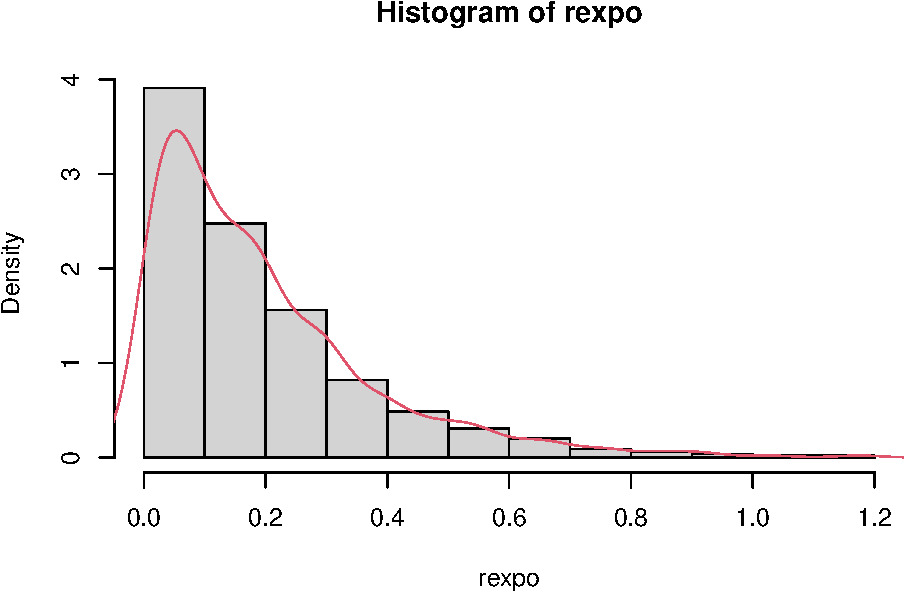
\includegraphics{A3Simulacion_files/figure-latex/unnamed-chunk-4-1.pdf}
\caption{\label{fig:unnamed-chunk-4}Histograma de observaciones con distribución exponencial}
\end{figure}

\hypertarget{muxe9todo-de-la-grilla}{%
\subsection{Método de la grilla}\label{muxe9todo-de-la-grilla}}

Existen distribuciones de probabilidad cuya forma estructural es muy compleja. Mas aún, existen distribuciones de probabilidad conocidas para las cuales la inversa de la función de de densidad acumulativa es difícil de solucionar analíticamente. En los anteriores casos, el método analítico dado por el teorema de la transformación integral de probabilidad no siempre resulta efectivo. Sin embargo, es posible realizar una variante, manteniendo el espíritu de la anterior técnica.

El presente método utiliza una distribución discreta para aproximar cualquier tipo de distribución (discreta o continua) sin importar su nivel de complejidad. El algoritmo que enmarca este método se da a continuación:

\begin{enumerate}
\def\labelenumi{\arabic{enumi}.}
\tightlist
\item
  Escribir la densidad de interés como \(f(\cdot)\) y establecer el rango de la variable aleatoria de interés.
\item
  Fijar un conjunto de \(n\) valores \(x_1<\cdots<x_n\) equiespaciados que cubran una gran parte del rango de la variable aleatoria.
\item
  Para \(x_k\) \((k=1,\ldots,n)\) calcular \(f(x_k)\) que equivale al valor de la densidad en el punto \(x_k\). Nótese que si \(f(\cdot)\) es una función de densidad continua, entonces \(f(x_k)\) no corresponde a una probabilidad;
\item
  Calcular la probabilidad asociada al punto \(x_k\) definida por la aproximación discreta a \(f(\cdot)\) y dada por
  \begin{equation*}
  p(x_k)=\frac{f(x_k)}{\sum_{k=1}^{n}f(x_k)}
  \end{equation*}
\item
  Calcular la función de densidad acumulativa aproximada definida como
  \begin{equation*}
  F(x)=
  \begin{cases}
  0, \ \ \ \text{si $x<x_1$}\\
  \sum_{l=1}^kp(x_l), \ \ \ \text{si $x_k\leq x<x_{k+1}$}\\
  1, \ \ \ \text{si $x>x_n$}
  \end{cases}
  \end{equation*}
\item
  Simular una observación \(u\) proveniente de una distribución uniforme continua en el intervalo \((0,1)\).
\item
  Si \(F(x_k)<u\leq F(x_{k+1})\), entonces \(F^{-1}(u)=x_{k+1}\) y por consiguiente el valor \(x_{k+1}\) es una pseudo-observación proveniente de la densidad de interés.
\end{enumerate}

Nótese que en el anterior proceso, la unidad \(x_{k+1}\) es seleccionada con probabilidad \(p_{k+1}\); puesto que

\begin{align*}
P(F(x_k)< U \leq F(x_{k+1}))&=F(x_{k+1})-F(x_{k})\\
&=\sum_{l=1}^{k+1}p(x_l)-\sum_{l=1}^kp(x_l)=p_{k+1}
\end{align*}

Si se quiere extraer una muestra aleatoria de \(N\) observaciones provenientes de la distribución de interés, entonces basta con repetir el anterior proceso \(N\) veces. Por supuesto, como se trata de una muestra aleatoria cada selección se debe realizar con repetición; de esta manera no importa si \(N>n\). Suponiendo que el conjunto \(x_1,\ldots,x_n\) conforma una grilla de puntos lo suficientemente cercanos y que no sucede nada importante entre cada uno de ellos, entonces esta técnica debe tener un buen funcionamiento.

\begin{example}
\protect\hypertarget{exm:unnamed-chunk-5}{}{\label{exm:unnamed-chunk-5} }El siguiente código computacional permite utilizar el método de la grilla para simular mil valores provenientes de una distribución exponencial con parámetro \(\theta = 5\).
\end{example}

\begin{Shaded}
\begin{Highlighting}[]
\NormalTok{theta }\OtherTok{\textless{}{-}} \DecValTok{5}
\NormalTok{x.grid }\OtherTok{\textless{}{-}} \FunctionTok{seq}\NormalTok{(}\DecValTok{0}\NormalTok{, }\DecValTok{100}\NormalTok{, }\AttributeTok{by=}\FloatTok{0.01}\NormalTok{)}
\NormalTok{p.exp }\OtherTok{\textless{}{-}}\NormalTok{ theta }\SpecialCharTok{*} \FunctionTok{exp}\NormalTok{(}\SpecialCharTok{{-}}\NormalTok{theta }\SpecialCharTok{*}\NormalTok{ x.grid)}
\NormalTok{r.exp }\OtherTok{\textless{}{-}} \FunctionTok{sample}\NormalTok{(x.grid, }\DecValTok{1000}\NormalTok{, }\AttributeTok{prob =}\NormalTok{ p.exp, }\AttributeTok{replace =}\NormalTok{ T)}
\DecValTok{1}\SpecialCharTok{/}\FunctionTok{mean}\NormalTok{(r.exp)}
\end{Highlighting}
\end{Shaded}

\begin{verbatim}
## [1] 4.805151
\end{verbatim}

\begin{Shaded}
\begin{Highlighting}[]
\FunctionTok{hist}\NormalTok{(r.exp, }\AttributeTok{freq =} \ConstantTok{FALSE}\NormalTok{)}
\FunctionTok{lines}\NormalTok{(}\FunctionTok{density}\NormalTok{(rexpo), }\AttributeTok{col =} \DecValTok{2}\NormalTok{)}
\end{Highlighting}
\end{Shaded}

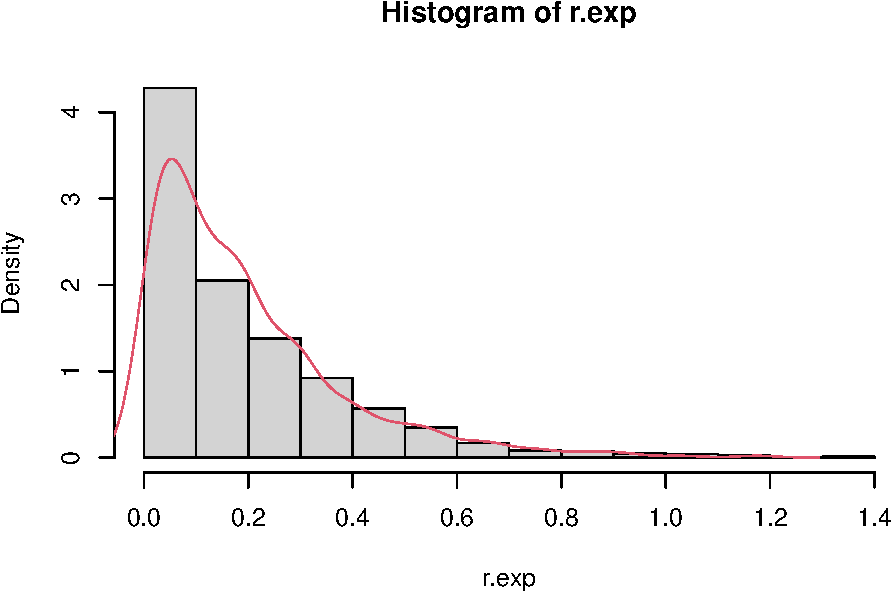
\includegraphics{A3Simulacion_files/figure-latex/unnamed-chunk-6-1.pdf}
\begin{example}
\protect\hypertarget{exm:unnamed-chunk-7}{}{\label{exm:unnamed-chunk-7} }De la misma manera, el método de la grilla permite simular valores de un distribución discreta. El siguiente código computacional permite utilizar el método de la grilla para simular mil valores provenientes de una distribución Poisson con parámetro \(\theta = 2\).
\end{example}

\begin{Shaded}
\begin{Highlighting}[]
\NormalTok{p.poisson }\OtherTok{\textless{}{-}}\ControlFlowTok{function}\NormalTok{(theta, x.grid)\{}
\NormalTok{  N }\OtherTok{\textless{}{-}} \FunctionTok{length}\NormalTok{(x.grid)}
\NormalTok{  res }\OtherTok{\textless{}{-}} \FunctionTok{rep}\NormalTok{(}\ConstantTok{NA}\NormalTok{, N)}
  \ControlFlowTok{for}\NormalTok{(k }\ControlFlowTok{in} \DecValTok{1}\SpecialCharTok{:}\NormalTok{N)\{}
\NormalTok{    P1 }\OtherTok{\textless{}{-}} \FunctionTok{exp}\NormalTok{(}\SpecialCharTok{{-}}\NormalTok{theta) }\SpecialCharTok{*}\NormalTok{ theta}\SpecialCharTok{\^{}}\NormalTok{(x.grid[k])}
\NormalTok{    P2 }\OtherTok{\textless{}{-}} \FunctionTok{factorial}\NormalTok{(x.grid[k])}
\NormalTok{    res[k] }\OtherTok{\textless{}{-}}\NormalTok{ P1}\SpecialCharTok{/}\NormalTok{P2}
\NormalTok{  \}}
  \FunctionTok{return}\NormalTok{(res)}
\NormalTok{\}}

\NormalTok{theta }\OtherTok{\textless{}{-}} \DecValTok{2}
\NormalTok{x.grid }\OtherTok{\textless{}{-}} \FunctionTok{seq}\NormalTok{(}\DecValTok{0}\NormalTok{, }\DecValTok{100}\NormalTok{, }\AttributeTok{by =} \DecValTok{1}\NormalTok{)}
\NormalTok{f.x }\OtherTok{\textless{}{-}} \FunctionTok{p.poisson}\NormalTok{(theta, x.grid)}
\NormalTok{p.x }\OtherTok{\textless{}{-}}\NormalTok{ f.x}\SpecialCharTok{/}\FunctionTok{sum}\NormalTok{(f.x)}
\FunctionTok{sum}\NormalTok{(p.x)}
\end{Highlighting}
\end{Shaded}

\begin{verbatim}
## [1] 1
\end{verbatim}

\begin{Shaded}
\begin{Highlighting}[]
\NormalTok{rpois }\OtherTok{\textless{}{-}} \FunctionTok{sample}\NormalTok{(x.grid, }\DecValTok{1000}\NormalTok{, }\AttributeTok{prob=}\NormalTok{p.x, }\AttributeTok{replace =}\NormalTok{ T)}
\FunctionTok{mean}\NormalTok{(rpois)}
\end{Highlighting}
\end{Shaded}

\begin{verbatim}
## [1] 2.013
\end{verbatim}

\begin{Shaded}
\begin{Highlighting}[]
\FunctionTok{var}\NormalTok{(rpois)}
\end{Highlighting}
\end{Shaded}

\begin{verbatim}
## [1] 1.972804
\end{verbatim}

\begin{Shaded}
\begin{Highlighting}[]
\FunctionTok{hist}\NormalTok{(rpois, }\AttributeTok{freq =} \ConstantTok{FALSE}\NormalTok{)}
\end{Highlighting}
\end{Shaded}

\begin{figure}
\centering
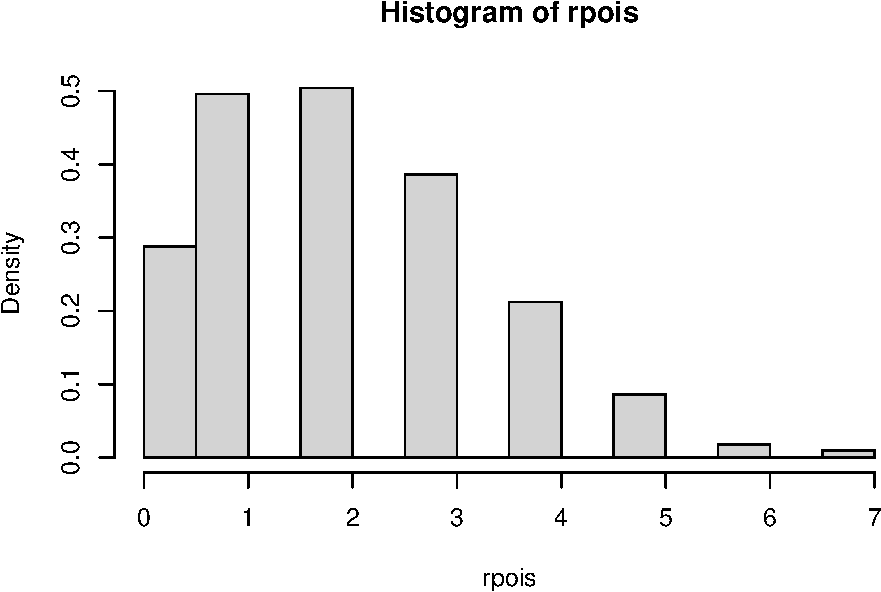
\includegraphics{A3Simulacion_files/figure-latex/unnamed-chunk-8-1.pdf}
\caption{\label{fig:unnamed-chunk-8}Histograma de observaciones con distribución Poisson}
\end{figure}

\begin{example}
\protect\hypertarget{exm:unnamed-chunk-9}{}{\label{exm:unnamed-chunk-9} }El método de la grilla también puede utilizarse para simular observaciones de una distribución biparamétrica, univariada y continua. El siguiente código computacional permite utilizar el método de la grilla para simular mil valores provenientes de una distribución Gamma con parámetros \(\theta = 4\), \(\beta = 2\).
\end{example}

\begin{Shaded}
\begin{Highlighting}[]
\NormalTok{p.gamma }\OtherTok{\textless{}{-}} \ControlFlowTok{function}\NormalTok{(a, b, x.grid)\{}
\NormalTok{  N }\OtherTok{\textless{}{-}}\FunctionTok{length}\NormalTok{(x.grid)}
\NormalTok{  res }\OtherTok{\textless{}{-}} \FunctionTok{rep}\NormalTok{(}\ConstantTok{NA}\NormalTok{, N)}
  \ControlFlowTok{for}\NormalTok{(k }\ControlFlowTok{in} \DecValTok{1}\SpecialCharTok{:}\NormalTok{N)\{}
\NormalTok{    P1 }\OtherTok{\textless{}{-}}\NormalTok{ (b}\SpecialCharTok{\^{}}\NormalTok{a)}\SpecialCharTok{/}\FunctionTok{gamma}\NormalTok{(a)}
\NormalTok{    P2 }\OtherTok{\textless{}{-}}\NormalTok{ x.grid[k]}\SpecialCharTok{\^{}}\NormalTok{(a }\SpecialCharTok{{-}} \DecValTok{1}\NormalTok{)}
\NormalTok{    P3 }\OtherTok{\textless{}{-}} \FunctionTok{exp}\NormalTok{(}\SpecialCharTok{{-}}\NormalTok{b }\SpecialCharTok{*}\NormalTok{ x.grid[k])}
\NormalTok{    res[k] }\OtherTok{\textless{}{-}}\NormalTok{ P1}\SpecialCharTok{*}\NormalTok{P2}\SpecialCharTok{*}\NormalTok{P3}
\NormalTok{  \}}
  \FunctionTok{return}\NormalTok{(res)}
\NormalTok{\}}

\NormalTok{alpha }\OtherTok{\textless{}{-}} \DecValTok{4}
\NormalTok{beta }\OtherTok{\textless{}{-}} \DecValTok{2}
\NormalTok{x.grid }\OtherTok{\textless{}{-}} \FunctionTok{seq}\NormalTok{(}\DecValTok{0}\NormalTok{, }\DecValTok{100}\NormalTok{, }\AttributeTok{by =} \FloatTok{0.1}\NormalTok{)}
\NormalTok{f.x }\OtherTok{\textless{}{-}} \FunctionTok{p.gamma}\NormalTok{(alpha, beta, x.grid)}
\NormalTok{p.x }\OtherTok{\textless{}{-}}\NormalTok{ f.x }\SpecialCharTok{/} \FunctionTok{sum}\NormalTok{(f.x)}

\NormalTok{rgamma }\OtherTok{\textless{}{-}} \FunctionTok{sample}\NormalTok{(x.grid, }\DecValTok{1000}\NormalTok{, }\AttributeTok{prob =}\NormalTok{ p.x, }\AttributeTok{replace =}\NormalTok{ T)}
\FunctionTok{mean}\NormalTok{(rgamma)}
\end{Highlighting}
\end{Shaded}

\begin{verbatim}
## [1] 1.9975
\end{verbatim}

\begin{Shaded}
\begin{Highlighting}[]
\FunctionTok{var}\NormalTok{(rgamma)}
\end{Highlighting}
\end{Shaded}

\begin{verbatim}
## [1] 1.031415
\end{verbatim}

\begin{Shaded}
\begin{Highlighting}[]
\FunctionTok{hist}\NormalTok{(rgamma, }\AttributeTok{freq =}\NormalTok{ F)}
\FunctionTok{lines}\NormalTok{(}\FunctionTok{density}\NormalTok{(rgamma), }\AttributeTok{col =} \DecValTok{2}\NormalTok{)}
\end{Highlighting}
\end{Shaded}

\begin{figure}
\centering
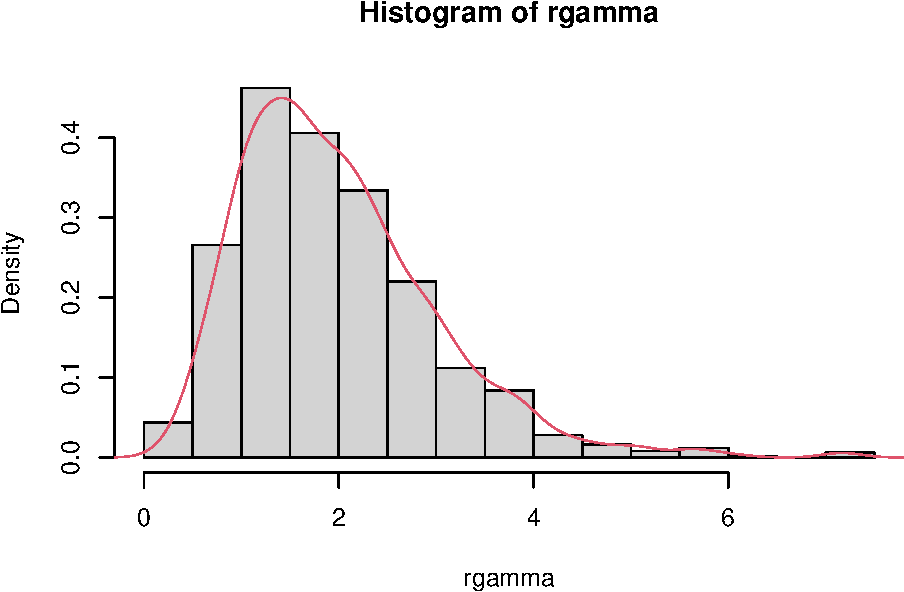
\includegraphics{A3Simulacion_files/figure-latex/unnamed-chunk-10-1.pdf}
\caption{\label{fig:unnamed-chunk-10}Histograma de observaciones con distribución Gamma.}
\end{figure}

\begin{example}
\protect\hypertarget{exm:unnamed-chunk-11}{}{\label{exm:unnamed-chunk-11} }Para comprobar el poder de este método de simulación, se presenta el siguiente código que permite simular valores de una distribución multiparamétrica, bivariada y continua. En particular, se simulan valores de la distribución Normal multivariante con vector de medias \(\boldsymbol \mu= (2, 4)'\) y matriz de varianzas covarianzas
\(\boldsymbol \Sigma= \begin{bmatrix} 25 & 30 \\ 30 & 16 \end{bmatrix}\)
\end{example}

\begin{Shaded}
\begin{Highlighting}[]
\NormalTok{p.normal2 }\OtherTok{\textless{}{-}} \ControlFlowTok{function}\NormalTok{(mu, Sigma, x, y)\{}
\NormalTok{  P1  }\OtherTok{\textless{}{-}} \DecValTok{1}\SpecialCharTok{/}\NormalTok{(}\DecValTok{2} \SpecialCharTok{*}\NormalTok{ pi)}
\NormalTok{  P2  }\OtherTok{\textless{}{-}} \DecValTok{1}\SpecialCharTok{/}\FunctionTok{sqrt}\NormalTok{(}\FunctionTok{det}\NormalTok{(Sigma))}
\NormalTok{  P3a }\OtherTok{\textless{}{-}} \FunctionTok{t}\NormalTok{((}\FunctionTok{c}\NormalTok{(x, y) }\SpecialCharTok{{-}}\NormalTok{ mu)) }\SpecialCharTok{\%*\%} \FunctionTok{solve}\NormalTok{(Sigma) }\SpecialCharTok{\%*\%}\NormalTok{ (}\FunctionTok{c}\NormalTok{(x, y) }\SpecialCharTok{{-}}\NormalTok{ mu)}
\NormalTok{  P3  }\OtherTok{\textless{}{-}} \FunctionTok{exp}\NormalTok{((}\SpecialCharTok{{-}}\DecValTok{1}\SpecialCharTok{/}\DecValTok{2}\NormalTok{) }\SpecialCharTok{*}\NormalTok{ P3a)}
\NormalTok{  res }\OtherTok{\textless{}{-}}\NormalTok{ P1 }\SpecialCharTok{*}\NormalTok{ P2 }\SpecialCharTok{*}\NormalTok{ P3}
  \FunctionTok{return}\NormalTok{(res)}
\NormalTok{\}}

\NormalTok{grilla }\OtherTok{\textless{}{-}} \ControlFlowTok{function}\NormalTok{(a, b)\{}
\NormalTok{  A }\OtherTok{\textless{}{-}} \FunctionTok{seq}\NormalTok{(}\DecValTok{1}\SpecialCharTok{:}\FunctionTok{length}\NormalTok{(a))}
\NormalTok{  unoA }\OtherTok{\textless{}{-}} \FunctionTok{rep}\NormalTok{(}\DecValTok{1}\NormalTok{, }\FunctionTok{length}\NormalTok{(A))}
\NormalTok{  B }\OtherTok{\textless{}{-}} \FunctionTok{seq}\NormalTok{(}\DecValTok{1}\SpecialCharTok{:}\FunctionTok{length}\NormalTok{(b))}
\NormalTok{  unoB }\OtherTok{\textless{}{-}} \FunctionTok{rep}\NormalTok{(}\DecValTok{1}\NormalTok{, }\FunctionTok{length}\NormalTok{(B))}
\NormalTok{  P1 }\OtherTok{\textless{}{-}} \FunctionTok{kronecker}\NormalTok{(A, unoB)}
\NormalTok{  P2 }\OtherTok{\textless{}{-}} \FunctionTok{kronecker}\NormalTok{(unoA, B)}
\NormalTok{  grid }\OtherTok{\textless{}{-}} \FunctionTok{cbind}\NormalTok{(a[P1], b[P2])}
  \FunctionTok{return}\NormalTok{(grid)}
\NormalTok{\}}

\NormalTok{mu1 }\OtherTok{\textless{}{-}} \FunctionTok{c}\NormalTok{(}\DecValTok{2}\NormalTok{, }\DecValTok{4}\NormalTok{)}
\NormalTok{Sigma1 }\OtherTok{\textless{}{-}} \FunctionTok{matrix}\NormalTok{(}\FunctionTok{c}\NormalTok{(}\DecValTok{25}\NormalTok{, }\DecValTok{10}\NormalTok{, }\DecValTok{10}\NormalTok{, }\DecValTok{16}\NormalTok{), }\AttributeTok{nrow=}\DecValTok{2}\NormalTok{)}

\NormalTok{x.grid }\OtherTok{\textless{}{-}} \FunctionTok{seq}\NormalTok{(mu1[}\DecValTok{1}\NormalTok{] }\SpecialCharTok{{-}} \DecValTok{3} \SpecialCharTok{*} \FunctionTok{sqrt}\NormalTok{(Sigma1[}\DecValTok{1}\NormalTok{, }\DecValTok{1}\NormalTok{]),}
\NormalTok{              mu1[}\DecValTok{1}\NormalTok{] }\SpecialCharTok{+} \DecValTok{3} \SpecialCharTok{*} \FunctionTok{sqrt}\NormalTok{(Sigma1[}\DecValTok{1}\NormalTok{, }\DecValTok{1}\NormalTok{]),}
              \AttributeTok{by =} \FloatTok{0.5}\NormalTok{)}
\NormalTok{y.grid }\OtherTok{\textless{}{-}} \FunctionTok{seq}\NormalTok{(mu1[}\DecValTok{2}\NormalTok{] }\SpecialCharTok{{-}} \DecValTok{3} \SpecialCharTok{*} \FunctionTok{sqrt}\NormalTok{(Sigma1[}\DecValTok{2}\NormalTok{, }\DecValTok{2}\NormalTok{]),}
\NormalTok{              mu1[}\DecValTok{2}\NormalTok{] }\SpecialCharTok{+} \DecValTok{3} \SpecialCharTok{*} \FunctionTok{sqrt}\NormalTok{(Sigma1[}\DecValTok{2}\NormalTok{, }\DecValTok{2}\NormalTok{]),}
              \AttributeTok{by =} \FloatTok{0.5}\NormalTok{)}
\NormalTok{xy.grid }\OtherTok{\textless{}{-}} \FunctionTok{grilla}\NormalTok{(x.grid, y.grid)}
\NormalTok{N.grid }\OtherTok{\textless{}{-}} \FunctionTok{dim}\NormalTok{(xy.grid)[}\DecValTok{1}\NormalTok{]}

\NormalTok{f.xy }\OtherTok{\textless{}{-}} \FunctionTok{rep}\NormalTok{(}\ConstantTok{NA}\NormalTok{, N.grid)}
\ControlFlowTok{for}\NormalTok{(j }\ControlFlowTok{in} \DecValTok{1}\SpecialCharTok{:}\NormalTok{N.grid)\{}
\NormalTok{  f.xy[j] }\OtherTok{\textless{}{-}} \FunctionTok{p.normal2}\NormalTok{(mu1, Sigma1, }
\NormalTok{                       xy.grid[j, }\DecValTok{1}\NormalTok{], }
\NormalTok{                       xy.grid[j, }\DecValTok{2}\NormalTok{])}
\NormalTok{\}}

\NormalTok{p.xy }\OtherTok{\textless{}{-}} \FunctionTok{as.vector}\NormalTok{(f.xy}\SpecialCharTok{/}\FunctionTok{sum}\NormalTok{(f.xy))}
\FunctionTok{sum}\NormalTok{(p.xy)}
\end{Highlighting}
\end{Shaded}

\begin{verbatim}
## [1] 1
\end{verbatim}

\begin{Shaded}
\begin{Highlighting}[]
\NormalTok{rnormal2 }\OtherTok{\textless{}{-}} \FunctionTok{sample}\NormalTok{(N.grid, }\DecValTok{1000}\NormalTok{, }\AttributeTok{prob =}\NormalTok{ p.xy, }\AttributeTok{replace =}\NormalTok{ T)}
\NormalTok{rxy.normal2 }\OtherTok{\textless{}{-}}\NormalTok{ xy.grid[rnormal2, ]}
\NormalTok{rx.normal }\OtherTok{\textless{}{-}}\NormalTok{ rxy.normal2[, }\DecValTok{1}\NormalTok{]}
\NormalTok{ry.normal }\OtherTok{\textless{}{-}}\NormalTok{ rxy.normal2[, }\DecValTok{2}\NormalTok{]}

\FunctionTok{colMeans}\NormalTok{(rxy.normal2)}
\end{Highlighting}
\end{Shaded}

\begin{verbatim}
## [1] 1.678 3.976
\end{verbatim}

\begin{Shaded}
\begin{Highlighting}[]
\FunctionTok{var}\NormalTok{(rxy.normal2)}
\end{Highlighting}
\end{Shaded}

\begin{verbatim}
##           [,1]      [,2]
## [1,] 24.955271  9.292064
## [2,]  9.292064 14.929353
\end{verbatim}

\begin{Shaded}
\begin{Highlighting}[]
\FunctionTok{hist}\NormalTok{(rx.normal, }\AttributeTok{freq =}\NormalTok{ F)}
\FunctionTok{lines}\NormalTok{(}\FunctionTok{density}\NormalTok{(rx.normal), }\AttributeTok{col =} \DecValTok{2}\NormalTok{)}
\end{Highlighting}
\end{Shaded}

\begin{figure}
\centering
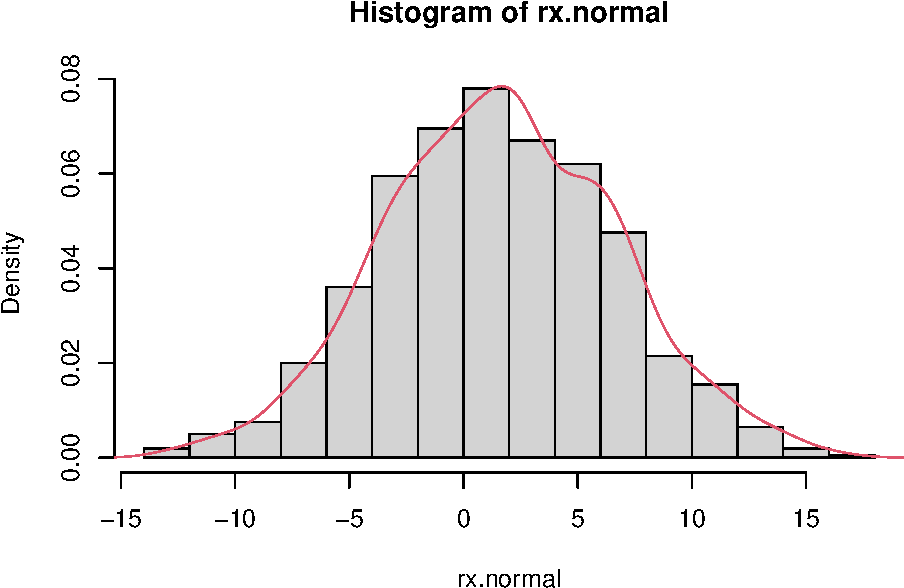
\includegraphics{A3Simulacion_files/figure-latex/unnamed-chunk-12-1.pdf}
\caption{\label{fig:unnamed-chunk-12-1}Histogramas de observaciones con distribución Normal bivariada.}
\end{figure}

\begin{Shaded}
\begin{Highlighting}[]
\FunctionTok{hist}\NormalTok{(ry.normal, }\AttributeTok{freq =}\NormalTok{ F)}
\FunctionTok{lines}\NormalTok{(}\FunctionTok{density}\NormalTok{(ry.normal), }\AttributeTok{col =} \DecValTok{2}\NormalTok{)}
\end{Highlighting}
\end{Shaded}

\begin{figure}
\centering
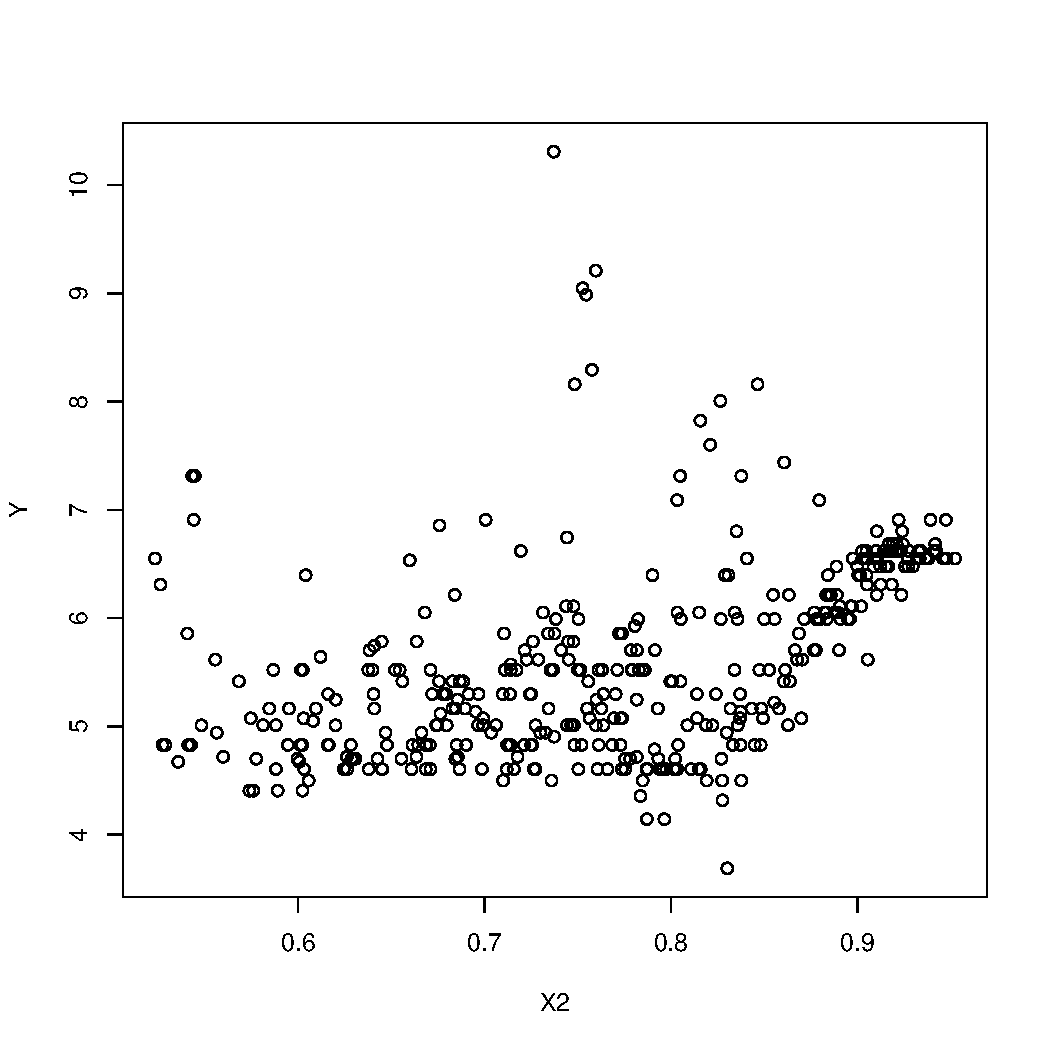
\includegraphics{A3Simulacion_files/figure-latex/unnamed-chunk-12-2.pdf}
\caption{\label{fig:unnamed-chunk-12-2}Histogramas de observaciones con distribución Normal bivariada.}
\end{figure}

\hypertarget{muxe9todos-de-monte-carlo-vuxeda-cadenas-de-markov}{%
\section{Métodos de Monte Carlo vía cadenas de Markov}\label{muxe9todos-de-monte-carlo-vuxeda-cadenas-de-markov}}

\hypertarget{el-muestreador-de-gibbs}{%
\subsection{El muestreador de Gibbs}\label{el-muestreador-de-gibbs}}

Tal como lo afirma \citet{Pena2002}, este procedimiento es apropiado para obtener muestras de una distribución
conjunta cuando es fácil muestrear de las distribuciones condicionadas. El algoritmo se implementa asumiendo que \(\boldsymbol \theta_i=(\theta^{(1)}_i, . . . , \theta^{(d)}_i)\) representa a los valores actuales de \(\boldsymbol \theta\). Entonces \(\boldsymbol \theta_{i+1}\) se obtiene así:

\begin{itemize}
\tightlist
\item
  Generar \(\theta^{(1)}_{i+1}\) de \(p(\theta^{(1)} \mid \theta^{(2)}_i, \ldots,\theta^{(d)}_i,x)\)
\item
  Generar \(\theta^{(2)}_{i+1}\) de \(p(\theta^{(2)} \mid \theta^{(1)}_{i+1}, \theta^{(3)}_i, \ldots , \theta^{(d)}_i, x)\)
\item
  \(\ldots\)
\item
  Generar \(\theta^{(d)}_{i+1}\) de \(p(\theta^{(d)} \mid \theta^{(1)}_{i+1}, \theta^{(2)}_{i+1}, \ldots , \theta^{(d-1)}_{i+1} , x)\)
\end{itemize}

La idea de este esquema es renovar cada componente por medio de la simulación de la correspondiente distribución condicional. Una vez que la cadena converge, se tiene que los valores de \(\boldsymbol \theta\) corresponden a observaciones de la distribución requerida, \(p(\boldsymbol \theta\mid x)\). Sin embargo, en general, no se garantiza una muestra variables aleatorias \emph{totalmente} independientes provenientes de la distribución \(p(\theta \mid x)\), dado que el esquema del muestreador de Gibbs usa el valor actual para construir el siguiente valor; por ende, la secuencia de valores que se obtiene estará correlacionada.

\begin{example}
\protect\hypertarget{exm:unnamed-chunk-13}{}{\label{exm:unnamed-chunk-13} }Se puede implementar el muestreador de Gibbs para generar una secuencia de observaciones con densidad
conjunta

\begin{equation*}
(x,y) \sim N_2 \Bigl(0,
 \begin{pmatrix}
 \rho & 0 \\
 0 & \rho
 \end{pmatrix}
 \Bigl)
\end{equation*}

Teniendo en cuenta que la media de ambas variables es cero y su
varianza uno, entonces la covarianza entre ambas variables será \(\rho\) \citep{Robert}. Por ende, partiendo de valores iniciales \((x_t, y_t)\), el algoritmo se centra en actualizar las distribuciones condicionales según el resultado \ref{prp:normalmulti}.

\begin{align*}
x_{t+1}\mid y_t     & \sim N(\rho y_t, 1-\rho^2)\\
y_{t+1}\mid x_{t+1} & \sim N(\rho x_{t+1}, 1-\rho^2)
\end{align*}
\end{example}

\begin{Shaded}
\begin{Highlighting}[]
\NormalTok{bivariate.gibbs }\OtherTok{\textless{}{-}} \ControlFlowTok{function}\NormalTok{ (n, rho, x, y) \{}
\NormalTok{  mat }\OtherTok{\textless{}{-}} \FunctionTok{matrix}\NormalTok{(}\AttributeTok{ncol =} \DecValTok{2}\NormalTok{, }\AttributeTok{nrow =}\NormalTok{ n)}
\NormalTok{  mat[}\DecValTok{1}\NormalTok{, ] }\OtherTok{\textless{}{-}} \FunctionTok{c}\NormalTok{(x, y)}
  \ControlFlowTok{for}\NormalTok{ (i }\ControlFlowTok{in} \DecValTok{2}\SpecialCharTok{:}\NormalTok{n)\{}
\NormalTok{    x }\OtherTok{\textless{}{-}} \FunctionTok{rnorm}\NormalTok{(}\DecValTok{1}\NormalTok{, rho }\SpecialCharTok{*}\NormalTok{ y, }\FunctionTok{sqrt}\NormalTok{(}\DecValTok{1} \SpecialCharTok{{-}}\NormalTok{ rho}\SpecialCharTok{\^{}}\DecValTok{2}\NormalTok{))}
\NormalTok{    y }\OtherTok{\textless{}{-}} \FunctionTok{rnorm}\NormalTok{(}\DecValTok{1}\NormalTok{, rho }\SpecialCharTok{*}\NormalTok{ x, }\FunctionTok{sqrt}\NormalTok{(}\DecValTok{1} \SpecialCharTok{{-}}\NormalTok{ rho}\SpecialCharTok{\^{}}\DecValTok{2}\NormalTok{))}
\NormalTok{    mat[i, ] }\OtherTok{\textless{}{-}} \FunctionTok{c}\NormalTok{(x, y)}
\NormalTok{  \}}
\NormalTok{  mat}\OtherTok{\textless{}{-}}\FunctionTok{as.data.frame}\NormalTok{(mat)}
  \FunctionTok{return}\NormalTok{(mat)}
\NormalTok{\}}

\NormalTok{biv }\OtherTok{\textless{}{-}} \FunctionTok{bivariate.gibbs}\NormalTok{(}\AttributeTok{n=}\DecValTok{2000}\NormalTok{, }\AttributeTok{rho=}\FloatTok{0.5}\NormalTok{, }\AttributeTok{x=} \DecValTok{0}\NormalTok{, }\AttributeTok{y =} \DecValTok{0}\NormalTok{)}
\FunctionTok{colMeans}\NormalTok{(biv)}
\end{Highlighting}
\end{Shaded}

\begin{verbatim}
##           V1           V2 
## -0.009751821 -0.028181553
\end{verbatim}

\begin{Shaded}
\begin{Highlighting}[]
\FunctionTok{var}\NormalTok{(biv)}
\end{Highlighting}
\end{Shaded}

\begin{verbatim}
##           V1        V2
## V1 0.9705958 0.4782972
## V2 0.4782972 0.9944298
\end{verbatim}

\begin{Shaded}
\begin{Highlighting}[]
\FunctionTok{cor}\NormalTok{(biv)}
\end{Highlighting}
\end{Shaded}

\begin{verbatim}
##           V1        V2
## V1 1.0000000 0.4868459
## V2 0.4868459 1.0000000
\end{verbatim}

\begin{Shaded}
\begin{Highlighting}[]
\FunctionTok{plot}\NormalTok{(biv)}
\end{Highlighting}
\end{Shaded}

\begin{figure}
\centering
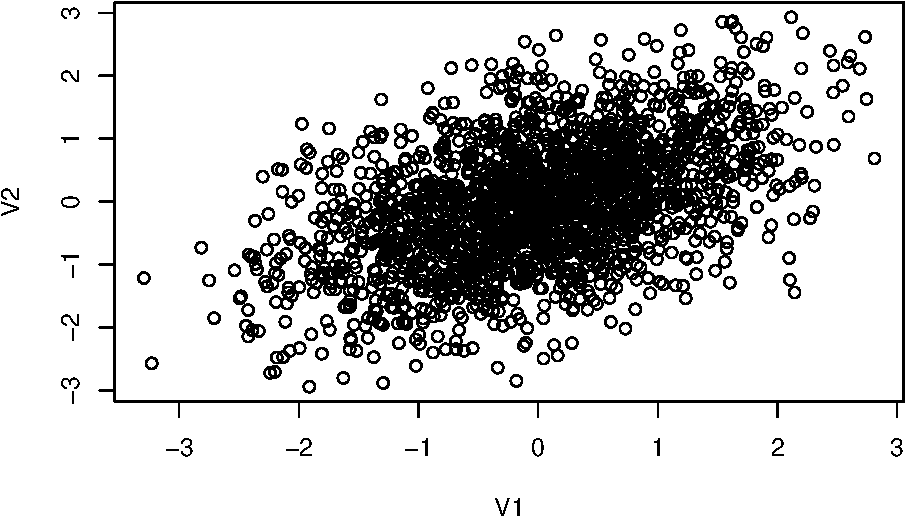
\includegraphics{A3Simulacion_files/figure-latex/unnamed-chunk-14-1.pdf}
\caption{\label{fig:unnamed-chunk-14}Generación de valores para una distribución normal bivariada.}
\end{figure}

\begin{example}
\protect\hypertarget{exm:unnamed-chunk-15}{}{\label{exm:unnamed-chunk-15} }Un problema común es el de descartar los primeros valores, puesto que el algoritmo puede demorar en obtener convergencia;
esto se puede resolver en forma empírica utilizando las medias y varianzas acumuladas y graficándolas se puede tomar una decisión acerca del valor óptimo en el que la cadena converge.

Con el siguiente código computacional, es posible corroborar que un punto de corte óptimo desde el cual se consideraría que las cadenas simuladas anteriormente es a partir de la iteración \textbf{600}.
\end{example}

\begin{Shaded}
\begin{Highlighting}[]
\NormalTok{g.diag }\OtherTok{\textless{}{-}} \ControlFlowTok{function}\NormalTok{(sample)\{}
\NormalTok{  n }\OtherTok{\textless{}{-}} \FunctionTok{length}\NormalTok{(sample) }
\NormalTok{  res }\OtherTok{\textless{}{-}} \FunctionTok{matrix}\NormalTok{(}\AttributeTok{nrow=}\DecValTok{2}\NormalTok{, }\AttributeTok{ncol=}\NormalTok{n)}
  \ControlFlowTok{for}\NormalTok{(i }\ControlFlowTok{in} \DecValTok{1}\SpecialCharTok{:}\NormalTok{n)\{}
\NormalTok{    res[}\DecValTok{1}\NormalTok{, i] }\OtherTok{\textless{}{-}} \FunctionTok{mean}\NormalTok{(sample[}\DecValTok{1} \SpecialCharTok{:}\NormalTok{ i])}
\NormalTok{    res[}\DecValTok{2}\NormalTok{, i] }\OtherTok{\textless{}{-}} \FunctionTok{var}\NormalTok{(sample[}\DecValTok{1} \SpecialCharTok{:}\NormalTok{ i])}
\NormalTok{  \}}
  \FunctionTok{return}\NormalTok{(res)}
\NormalTok{\}}

\NormalTok{m1 }\OtherTok{\textless{}{-}} \FunctionTok{g.diag}\NormalTok{(biv[, }\DecValTok{1}\NormalTok{])}
\NormalTok{m2 }\OtherTok{\textless{}{-}} \FunctionTok{g.diag}\NormalTok{(biv[, }\DecValTok{2}\NormalTok{])}

\FunctionTok{par}\NormalTok{(}\AttributeTok{mfcol =} \FunctionTok{c}\NormalTok{(}\DecValTok{1}\NormalTok{, }\DecValTok{2}\NormalTok{))}
\FunctionTok{plot}\NormalTok{(m1[}\DecValTok{1}\NormalTok{, ], }\AttributeTok{type =} \StringTok{\textquotesingle{}l\textquotesingle{}}\NormalTok{, }\AttributeTok{ylim=}\FunctionTok{c}\NormalTok{(}\SpecialCharTok{{-}}\FloatTok{0.6}\NormalTok{, }\FloatTok{0.6}\NormalTok{), }\AttributeTok{col=}\DecValTok{4}\NormalTok{)}
\FunctionTok{lines}\NormalTok{(m2[}\DecValTok{1}\NormalTok{, ], }\AttributeTok{lty =} \DecValTok{2}\NormalTok{, }\AttributeTok{col =} \DecValTok{2}\NormalTok{)}
\FunctionTok{title}\NormalTok{(}\StringTok{"Diagnóstico {-} Media acumulada"}\NormalTok{)}

\FunctionTok{plot}\NormalTok{(m1[}\DecValTok{2}\NormalTok{, ], }\AttributeTok{type =} \StringTok{\textquotesingle{}l\textquotesingle{}}\NormalTok{, }\AttributeTok{ylim =} \FunctionTok{c}\NormalTok{(}\FloatTok{0.5}\NormalTok{, }\FloatTok{1.5}\NormalTok{), }\AttributeTok{col=}\DecValTok{4}\NormalTok{)}
\FunctionTok{lines}\NormalTok{(m2[}\DecValTok{2}\NormalTok{, ], }\AttributeTok{lty =} \DecValTok{2}\NormalTok{, }\AttributeTok{col =} \DecValTok{2}\NormalTok{)}
\FunctionTok{title}\NormalTok{(}\StringTok{"Diagnóstico {-} Varianza acumulada"}\NormalTok{)}
\end{Highlighting}
\end{Shaded}

\begin{figure}
\centering
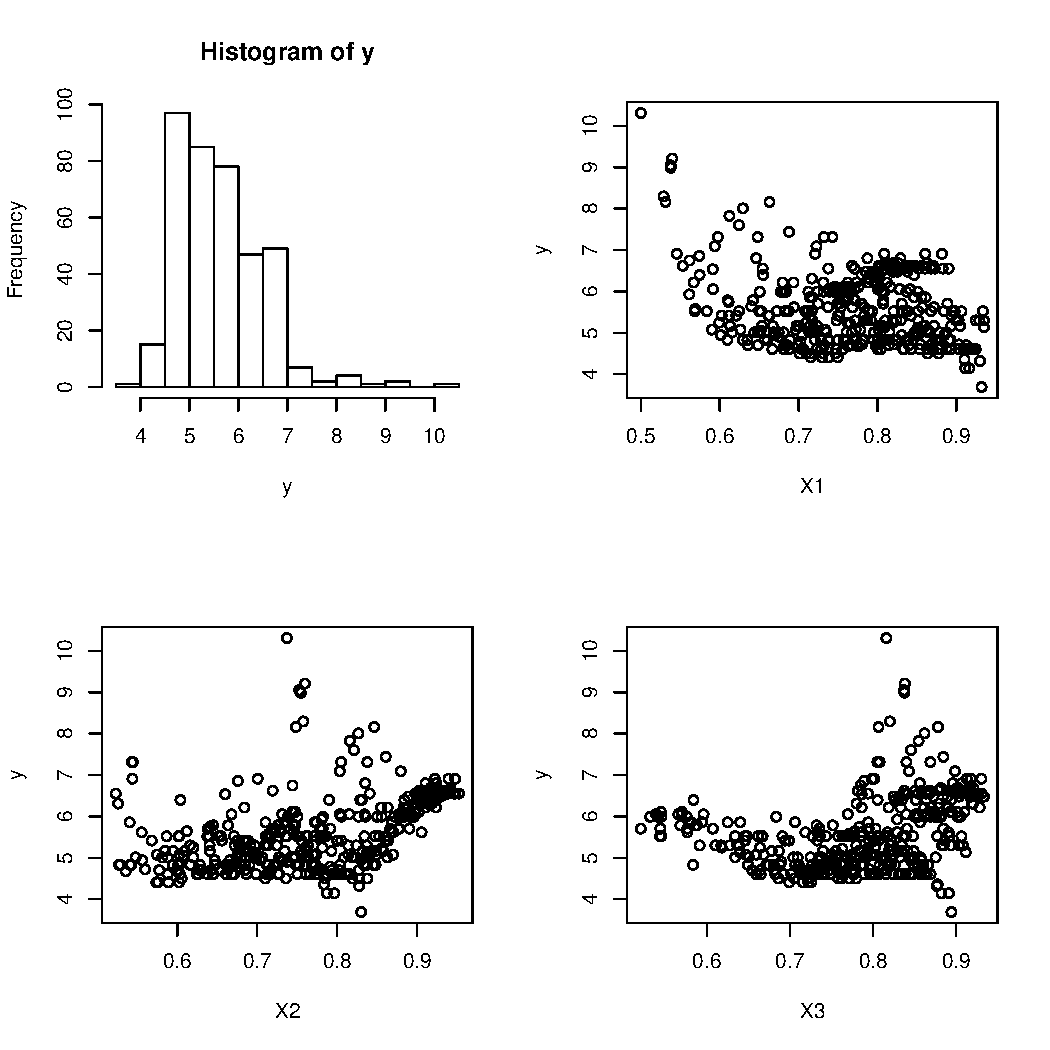
\includegraphics{A3Simulacion_files/figure-latex/unnamed-chunk-16-1.pdf}
\caption{\label{fig:unnamed-chunk-16}Convergencia de la media y varianza usando el muestreador de Gibbs.}
\end{figure}

El muestrador de Gibbs también funciona en una ``segunda fase'', cuando queremos seleccionar una muestra de \(f(\theta\mid x)\), es decir, la distribución de los parámetros dada la información observada \(x\).

\begin{example}
\protect\hypertarget{exm:GibbsN2}{}{\label{exm:GibbsN2} }Suponga que \(y\) tiene distribución \(N(\mu,\sigma^2=1/\phi)\) y queremos obtener una muestra de la distribución posterior del vector aleatorio \(\boldsymbol \theta=(\mu,1/\phi)\). Para este caso supongamos que conocemos las distribuciones previas; para la media \(\mu\) se asume una distribución uniforme y para la varianza \(\phi\) una distribución Gamma con parámetros \(a\) y \(b\). La distribución posterior de \((\mu, \phi)\) satisface:

\begin{equation}  
p(\mu, \phi \mid y) \propto (\phi)^{n/2}
\exp\left\{-\phi
\frac{\sum_{j=1}^n(y_j-\mu)^2}{2}\right\}(\phi)^{a-1}exp(-b/\phi)
\end{equation}

En donde la primera parte después del signo de proporcionalidad, corresponde a la verosimilitud de la información observada y la segunda parte corresponde a la distribución posterior de \(\phi\); la distribución posterior de \(\mu\) no
aparece pues es una constante. Por tanto, ésta se puede escribir como:

\begin{equation*}  
p(\mu, \phi \mid y)\propto(\phi)^{n/2+a-1}exp\left\{-\phi\Bigl(\frac{\sum_{j=1}^n(y_j-\mu)^2}{2}+b\Bigl)\right\}
\end{equation*}

Acudiendo al resultado \ref{prp:gammainver}, la distribución condicional de la varianza \(\sigma^2\) dado \((\mu, y)\) es Gamma-inversa con parámetros \(a+n/2\) y \(\sum_{j=1}^n(y_j-\mu)^2/2+b\). Por tanto,

\begin{equation} 
\label{eq:apmunormal}
\sigma^2\mid\mu,x\sim Gamma-inversa\biggl(\theta+n/2,\sum_{j=1}^n(y_j-\mu)^2/2+b\biggl)
\end{equation}

Análogamente, la distribución de \(\mu\) dado \((\sigma^2, y)\) es normal
con media \(\bar{y}\) y varianza \(\sigma^2/n\), es decir,

\begin{equation}  
\label{eq:apsigmaig}
\mu\mid\sigma^2,y\sim N(\bar{y},\sigma^2/n)
\end{equation}

Para implementar el muestreador de Gibbs con estas distribuciones, primero se deben escoger valores apropiados para \(a\) y \(b\), con el propósito de representar correctamente la
distribución previa, y luego

\begin{itemize}
\tightlist
\item
  Defninir un valor inicial para la media y la varianza, \((\mu_0, \sigma^2_0)\).
\item
  Generar \((\mu_{i+1}, \sigma_{i+1}^2)\) simulando \(\mu_{i+1}\) de \eqref{eq:apmunormal} y luego \(\sigma^2_{i+1}\) de \eqref{eq:apsigmaig}.
\item
  Iterar para obtener \((\mu_0, \sigma^2_0), (\mu_1, \sigma^2_1), (\mu_2, \sigma^2_2),\cdots,\).
\item
  Suponiendo que el algoritmo converge después de
  \(m\) iteraciones, descartar los \(m\) primeros valores.
\end{itemize}

Entonces \((\mu_{m+1}, \sigma^2_{m+1}), (\mu_{m+2}, \sigma^2_{m+2}),\cdots,\) es
una muestra (correlacionada) de \(p(\mu, \sigma^2\mid x)\).
\end{example}

La siguiente función en \texttt{R} implementa el muestreador de Gibbs para el anterior ejemplo.

\begin{Shaded}
\begin{Highlighting}[]
\FunctionTok{library}\NormalTok{(invgamma)}

\NormalTok{normal2 }\OtherTok{\textless{}{-}} \ControlFlowTok{function}\NormalTok{(datos, a, b, nsim, inicial)\{}
\NormalTok{  n }\OtherTok{\textless{}{-}} \FunctionTok{length}\NormalTok{(datos)}
\NormalTok{  xbar }\OtherTok{\textless{}{-}} \FunctionTok{mean}\NormalTok{(datos)}
\NormalTok{  mu.now }\OtherTok{\textless{}{-}}\NormalTok{ inicial[}\DecValTok{1}\NormalTok{]}
\NormalTok{  var.now }\OtherTok{\textless{}{-}}\NormalTok{ inicial[}\DecValTok{2}\NormalTok{]}
\NormalTok{  dummy }\OtherTok{\textless{}{-}} \FunctionTok{matrix}\NormalTok{(}\AttributeTok{ncol =} \DecValTok{2}\NormalTok{, }\AttributeTok{nrow =}\NormalTok{ nsim)}
\NormalTok{  dummy[}\DecValTok{1}\NormalTok{, }\DecValTok{1}\NormalTok{] }\OtherTok{\textless{}{-}}\NormalTok{ mu.now}
\NormalTok{  dummy[}\DecValTok{1}\NormalTok{, }\DecValTok{2}\NormalTok{] }\OtherTok{\textless{}{-}}\NormalTok{ var.now}
  
  \ControlFlowTok{for}\NormalTok{ (i }\ControlFlowTok{in} \DecValTok{2} \SpecialCharTok{:}\NormalTok{ nsim)\{}
\NormalTok{    alp }\OtherTok{\textless{}{-}}\NormalTok{ a }\SpecialCharTok{+}\NormalTok{ (n}\SpecialCharTok{/}\DecValTok{2}\NormalTok{)}
\NormalTok{    bet }\OtherTok{\textless{}{-}}\NormalTok{ b }\SpecialCharTok{+}\NormalTok{ (}\FunctionTok{sum}\NormalTok{((datos }\SpecialCharTok{{-}}\NormalTok{ mu.now)}\SpecialCharTok{\^{}}\DecValTok{2}\NormalTok{)}\SpecialCharTok{/}\DecValTok{2}\NormalTok{)}
\NormalTok{    var.next }\OtherTok{\textless{}{-}} \FunctionTok{rinvgamma}\NormalTok{(}\DecValTok{1}\NormalTok{, }\AttributeTok{shape =}\NormalTok{ alp, }\AttributeTok{rate =}\NormalTok{ bet)}
\NormalTok{    mu.next }\OtherTok{\textless{}{-}} \FunctionTok{rnorm}\NormalTok{(}\DecValTok{1}\NormalTok{, xbar, }\FunctionTok{sqrt}\NormalTok{(var.now}\SpecialCharTok{/}\NormalTok{n))}
\NormalTok{    dummy[i, }\DecValTok{1}\NormalTok{] }\OtherTok{\textless{}{-}}\NormalTok{ mu.next}
\NormalTok{    dummy[i, }\DecValTok{2}\NormalTok{] }\OtherTok{\textless{}{-}}\NormalTok{ var.next}
\NormalTok{    mu.now }\OtherTok{\textless{}{-}}\NormalTok{ mu.next}
\NormalTok{    var.now }\OtherTok{\textless{}{-}}\NormalTok{ var.next}
\NormalTok{  \}}
  \FunctionTok{return}\NormalTok{(dummy)}
\NormalTok{\}}

\NormalTok{datos }\OtherTok{\textless{}{-}} \FunctionTok{rnorm}\NormalTok{(}\DecValTok{100}\NormalTok{, }\DecValTok{5}\NormalTok{, }\DecValTok{2}\NormalTok{)}
\NormalTok{mc1.vals }\OtherTok{\textless{}{-}} \FunctionTok{normal2}\NormalTok{(datos, }\AttributeTok{a =} \DecValTok{2}\NormalTok{, }\AttributeTok{b =} \DecValTok{5}\NormalTok{, }
                    \AttributeTok{nsim =} \DecValTok{1000}\NormalTok{, }\AttributeTok{inicial =} \FunctionTok{c}\NormalTok{(}\DecValTok{2}\NormalTok{, }\DecValTok{2}\NormalTok{))}
\NormalTok{mc1.vals }\OtherTok{\textless{}{-}}\NormalTok{ mc1.vals[}\DecValTok{101}\SpecialCharTok{:} \DecValTok{1000}\NormalTok{, ]}
\FunctionTok{colMeans}\NormalTok{(mc1.vals)}
\end{Highlighting}
\end{Shaded}

\begin{verbatim}
## [1] 4.718260 4.056971
\end{verbatim}

\begin{Shaded}
\begin{Highlighting}[]
\FunctionTok{par}\NormalTok{(}\AttributeTok{mfcol =} \FunctionTok{c}\NormalTok{(}\DecValTok{1}\NormalTok{, }\DecValTok{2}\NormalTok{))}
\FunctionTok{plot}\NormalTok{(mc1.vals[, }\DecValTok{1}\NormalTok{], }\AttributeTok{type =} \StringTok{\textquotesingle{}l\textquotesingle{}}\NormalTok{, }\AttributeTok{ylab =} \StringTok{\textquotesingle{}mu\textquotesingle{}}\NormalTok{)}
\FunctionTok{plot}\NormalTok{(mc1.vals[, }\DecValTok{2}\NormalTok{], }\AttributeTok{type =} \StringTok{\textquotesingle{}l\textquotesingle{}}\NormalTok{, }\AttributeTok{ylab =} \StringTok{\textquotesingle{}sigma\^{}2\textquotesingle{}}\NormalTok{)}
\end{Highlighting}
\end{Shaded}

\begin{figure}
\centering
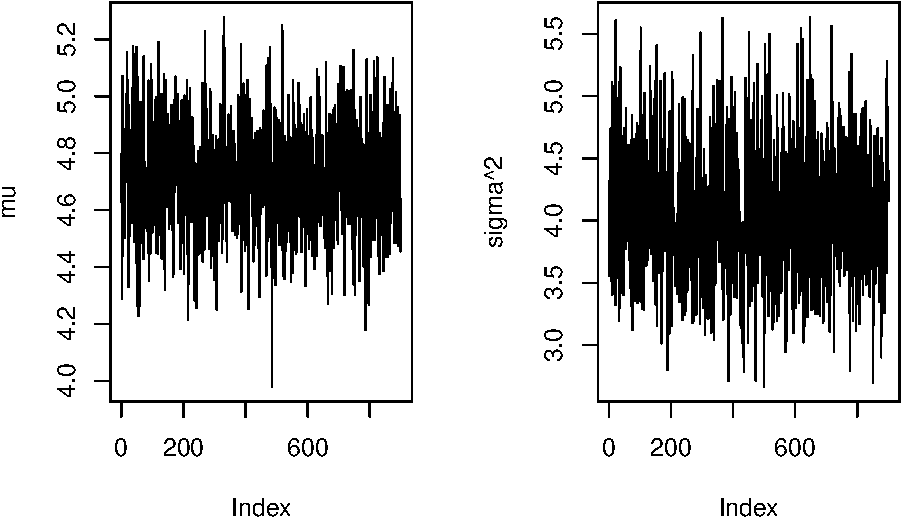
\includegraphics{A3Simulacion_files/figure-latex/unnamed-chunk-18-1.pdf}
\caption{\label{fig:unnamed-chunk-18}Cadenas generadas desde el muestreador de Gibbs.}
\end{figure}

\begin{Shaded}
\begin{Highlighting}[]
\FunctionTok{par}\NormalTok{(}\AttributeTok{mfcol =} \FunctionTok{c}\NormalTok{(}\DecValTok{1}\NormalTok{, }\DecValTok{2}\NormalTok{))}
\FunctionTok{hist}\NormalTok{(mc1.vals[, }\DecValTok{1}\NormalTok{], }\AttributeTok{prob =}\NormalTok{ T, }\AttributeTok{xlab=}\StringTok{\textquotesingle{}mu\textquotesingle{}}\NormalTok{, }\AttributeTok{main =} \StringTok{""}\NormalTok{)}
\FunctionTok{lines}\NormalTok{(}\FunctionTok{density}\NormalTok{(mc1.vals[, }\DecValTok{1}\NormalTok{], }\AttributeTok{kernel=}\StringTok{\textquotesingle{}gaussian\textquotesingle{}}\NormalTok{))}
\FunctionTok{hist}\NormalTok{(mc1.vals[, }\DecValTok{2}\NormalTok{], }\AttributeTok{prob =}\NormalTok{ T, }\AttributeTok{xlab=}\StringTok{\textquotesingle{}sigma\^{}2\textquotesingle{}}\NormalTok{, }\AttributeTok{main =} \StringTok{""}\NormalTok{)}
\FunctionTok{lines}\NormalTok{(}\FunctionTok{density}\NormalTok{(mc1.vals[, }\DecValTok{2}\NormalTok{], }\AttributeTok{kernel=}\StringTok{\textquotesingle{}gaussian\textquotesingle{}}\NormalTok{))}
\end{Highlighting}
\end{Shaded}

\begin{figure}
\centering
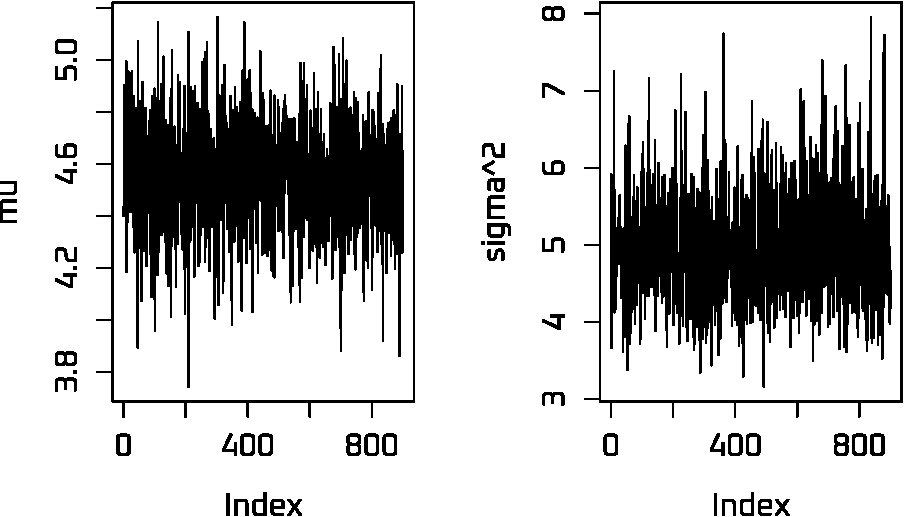
\includegraphics{A3Simulacion_files/figure-latex/unnamed-chunk-19-1.pdf}
\caption{\label{fig:unnamed-chunk-19}Densidades posteriores generadas con el muestreador de Gibbs.}
\end{figure}

\hypertarget{el-algoritmo-de-metruxf3polis-hastings}{%
\subsection{El algoritmo de Metrópolis-Hastings}\label{el-algoritmo-de-metruxf3polis-hastings}}

Este algoritmo se basa en proponer un nuevo punto de acuerdo a una función de densidad adecuada y aceptar este nuevo valor propuesto con una probabilidad que depende del punto actual, del nuevo punto y de la densidad de la cual fue propuesto el nuevo punto.

Suponga que deseamos simular valores de una distribución multivariada \(p(\theta \mid y)\). Sea la función de densidad propuesta \(q(\theta, \theta')\), una función de densidad de probabilidad arbitraria que
describe la probabilidad de aceptación de \(\theta'\) a partir de la posición actual de \(\theta\). El algoritmo de Metropolis-Hastings está dado por los siguientes pasos:

\begin{itemize}
\tightlist
\item
  Siendo el valor actual \(\theta_i\), genere un valor candidato \(\theta'\) obtenido como una observación de la densidad \(q(\theta_i, \theta')\).
\item
  Calcule
  \begin{equation*}
  T(\theta_i, \theta') =
  \begin{cases}
  \min \left(1,  \frac{p(\theta' \mid  y)q(\theta', \theta_i)}{p(\theta_i \mid  y)q(\theta_i, \theta')} \right),
  & \text{  si   } p(\theta_i \mid  y)q(\theta_i, \theta') > 0,\\ 
  1, & \text{  si   }
  p(\theta_i \mid y)q(\theta_i, \theta') = 0
  \end{cases}
  \end{equation*}
\item
  Acepte el nuevo valor y actualícelo a \(\theta_{i+1}=\theta'\) con probabilidad \(T(\theta_i, \theta')\). De otra forma, rechazar el valor candidato y defina \(\theta_{i+1}=\theta_i\).

  \item

  Repita el paso anterior para obtener la secuencia \(\theta_0,\theta_1,...,\)
  donde \(\theta_0\) denota un valor arbitrario de arranque.

  \item

  Descarte los primeros \(m\) valores obtenidos.
\end{itemize}

Siguiendo el anterior algoritmo, entonces se tiene que \(\theta_{m+1}, \theta_{m+2}, \ldots\) es una secuencia (correlacionada) de la distribución requerida. En principio, puede ser usada cualquier densidad \(q\), pero si ésta es escogida ingenuamente, la eficiencia de la cadena puede ser muy pobre. La relación más importante entre el muestreados de Gibbs y el algorítmo de Metropolis-Hastings, está dada como un teorema en el libro de \citet[pág. 296]{Robert}.

\begin{proposition}
\protect\hypertarget{prp:unnamed-chunk-20}{}{\label{prp:unnamed-chunk-20} }El muestreador de Gibbs es equivalente al algoritmo de Metropolis-Hastings, con la
probabilidad de aceptación igual a uno para todos los puntos propuestos.
\end{proposition}

Lo anterior implica que la convergencia para ambos métodos no es la misma. Para cerrar la sección de cadenas de Markov vía Monte Carlo, es importante hacernos la siguiente pregunta: ¿Son independientes las muestras simuladas? En principio no se puede hablar de independencia, pues es claro que la observación \(\{i+1\}\) depende de la observación \(\{i\}\). Dado que las observaciones resultantes
se encuentran en estricto orden de medición, podríamos utilizar algunos criterios como la función de auto-correlación (ACF) y la función de auto-correlación parcial (PACF), para conocer sobre la correlación entre observaciones.

Siguiendo con el ejemplo \ref{exm:GibbsN2} del apartado de Gibbs, se ha escogido usar como como distribuciones propuestas \(q\) para la media y para la varianza, densidades normales centradas en el actual
parámetro, ambas con varianza igual a uno. Dadas las distribuciones propuestas, algunos valores de la varianza pueden ser negativos; aunque este no es un problema porque la distribución posterior le asignará el valor cero, por tanto este valor será rechazado con un probabilidad de uno.

\begin{Shaded}
\begin{Highlighting}[]
\FunctionTok{library}\NormalTok{(invgamma)}

\NormalTok{met.hast }\OtherTok{\textless{}{-}} \ControlFlowTok{function}\NormalTok{(datos, a, b, iter, ini)\{}
\NormalTok{  mu0 }\OtherTok{\textless{}{-}}\NormalTok{ ini[}\DecValTok{1}\NormalTok{] }
\NormalTok{  var0 }\OtherTok{\textless{}{-}}\NormalTok{ ini[}\DecValTok{2}\NormalTok{]}
\NormalTok{  resul }\OtherTok{\textless{}{-}} \FunctionTok{matrix}\NormalTok{(}\AttributeTok{ncol =} \DecValTok{2}\NormalTok{, }\AttributeTok{nrow =}\NormalTok{ iter)}
\NormalTok{  resul[}\DecValTok{1}\NormalTok{, }\DecValTok{1}\NormalTok{] }\OtherTok{\textless{}{-}}\NormalTok{ mu0}
\NormalTok{  resul[}\DecValTok{1}\NormalTok{, }\DecValTok{2}\NormalTok{] }\OtherTok{\textless{}{-}}\NormalTok{ var0}
  \ControlFlowTok{for}\NormalTok{ (i }\ControlFlowTok{in} \DecValTok{2} \SpecialCharTok{:}\NormalTok{ iter)\{}
\NormalTok{    mu.prop }\OtherTok{\textless{}{-}} \FunctionTok{rnorm}\NormalTok{(}\DecValTok{1}\NormalTok{, mu0, }\DecValTok{1}\NormalTok{)}
\NormalTok{    var.prop }\OtherTok{\textless{}{-}} \FunctionTok{rnorm}\NormalTok{(}\DecValTok{1}\NormalTok{, var0, }\DecValTok{1}\NormalTok{)}
    \ControlFlowTok{if}\NormalTok{ (var.prop }\SpecialCharTok{\textless{}=} \DecValTok{0}\NormalTok{)\{ T.val }\OtherTok{\textless{}{-}} \DecValTok{0}\NormalTok{ \}}
    \ControlFlowTok{else}\NormalTok{\{}
\NormalTok{      p1 }\OtherTok{\textless{}{-}} \FunctionTok{prod}\NormalTok{(}\FunctionTok{dnorm}\NormalTok{(datos, mu.prop, }\FunctionTok{sqrt}\NormalTok{(var.prop))) }\SpecialCharTok{*}
        \FunctionTok{dinvgamma}\NormalTok{(var.prop, }\AttributeTok{shape =}\NormalTok{ a, }\AttributeTok{rate =}\NormalTok{ b)}
\NormalTok{      q1 }\OtherTok{\textless{}{-}} \FunctionTok{dnorm}\NormalTok{(mu0, mu.prop, }\DecValTok{1}\NormalTok{) }\SpecialCharTok{*}
        \FunctionTok{dnorm}\NormalTok{(var0, var.prop, }\DecValTok{1}\NormalTok{)}
\NormalTok{      p2 }\OtherTok{\textless{}{-}} \FunctionTok{prod}\NormalTok{(}\FunctionTok{dnorm}\NormalTok{(datos, mu0, }\FunctionTok{sqrt}\NormalTok{(var0))) }\SpecialCharTok{*} 
        \FunctionTok{dinvgamma}\NormalTok{(var0, }\AttributeTok{shape =}\NormalTok{ a, }\AttributeTok{rate =}\NormalTok{ b)}
\NormalTok{      q2 }\OtherTok{\textless{}{-}} \FunctionTok{dnorm}\NormalTok{(mu.prop, mu0, }\DecValTok{1}\NormalTok{) }\SpecialCharTok{*} 
        \FunctionTok{dnorm}\NormalTok{(var.prop, var0, }\DecValTok{1}\NormalTok{)}
\NormalTok{      T.val }\OtherTok{\textless{}{-}} \FunctionTok{min}\NormalTok{(}\DecValTok{1}\NormalTok{, (p1 }\SpecialCharTok{*}\NormalTok{ q1)}\SpecialCharTok{/}\NormalTok{(p2 }\SpecialCharTok{*}\NormalTok{ q2))}
\NormalTok{    \}}
\NormalTok{    u }\OtherTok{\textless{}{-}} \FunctionTok{runif}\NormalTok{(}\DecValTok{1}\NormalTok{) }
    \ControlFlowTok{if}\NormalTok{ (u }\SpecialCharTok{\textless{}=}\NormalTok{ T.val)\{}
\NormalTok{      resul[i, }\DecValTok{1}\NormalTok{] }\OtherTok{\textless{}{-}}\NormalTok{ mu.prop}
\NormalTok{      resul[i, }\DecValTok{2}\NormalTok{] }\OtherTok{\textless{}{-}}\NormalTok{ var.prop}
\NormalTok{      \} }
    \ControlFlowTok{else}\NormalTok{\{}
\NormalTok{      resul[i, }\DecValTok{1}\NormalTok{] }\OtherTok{\textless{}{-}}\NormalTok{ mu0}
\NormalTok{      resul[i, }\DecValTok{2}\NormalTok{] }\OtherTok{\textless{}{-}}\NormalTok{ var0}
\NormalTok{      \}}
\NormalTok{    mu0 }\OtherTok{\textless{}{-}}\NormalTok{ resul[i, }\DecValTok{1}\NormalTok{]}
\NormalTok{    var0 }\OtherTok{\textless{}{-}}\NormalTok{ resul[i, }\DecValTok{2}\NormalTok{]}
\NormalTok{  \}}
  \FunctionTok{return}\NormalTok{(resul)}
\NormalTok{\}}

\NormalTok{datos }\OtherTok{\textless{}{-}} \FunctionTok{rnorm}\NormalTok{(}\DecValTok{100}\NormalTok{, }\DecValTok{5}\NormalTok{, }\DecValTok{2}\NormalTok{)}
\NormalTok{mc2 }\OtherTok{\textless{}{-}} \FunctionTok{met.hast}\NormalTok{(datos, }\AttributeTok{a =} \DecValTok{2}\NormalTok{, }\AttributeTok{b =} \DecValTok{5}\NormalTok{, }
                \AttributeTok{iter =} \DecValTok{1000}\NormalTok{, }\AttributeTok{ini =} \FunctionTok{c}\NormalTok{(}\DecValTok{2}\NormalTok{, }\DecValTok{2}\NormalTok{))}
\FunctionTok{colMeans}\NormalTok{(mc2)}
\end{Highlighting}
\end{Shaded}

\begin{verbatim}
## [1] 4.729000 4.387919
\end{verbatim}

\begin{Shaded}
\begin{Highlighting}[]
\FunctionTok{par}\NormalTok{(}\AttributeTok{mfrow=}\FunctionTok{c}\NormalTok{(}\DecValTok{2}\NormalTok{,}\DecValTok{2}\NormalTok{))}
\FunctionTok{pacf}\NormalTok{(mc2[, }\DecValTok{1}\NormalTok{], }\DecValTok{100}\NormalTok{)}
\FunctionTok{pacf}\NormalTok{(mc2[, }\DecValTok{2}\NormalTok{], }\DecValTok{100}\NormalTok{)}
\FunctionTok{acf}\NormalTok{(mc2[, }\DecValTok{1}\NormalTok{], }\DecValTok{100}\NormalTok{)}
\FunctionTok{acf}\NormalTok{(mc2[, }\DecValTok{2}\NormalTok{], }\DecValTok{100}\NormalTok{)}
\end{Highlighting}
\end{Shaded}

\begin{figure}
\centering
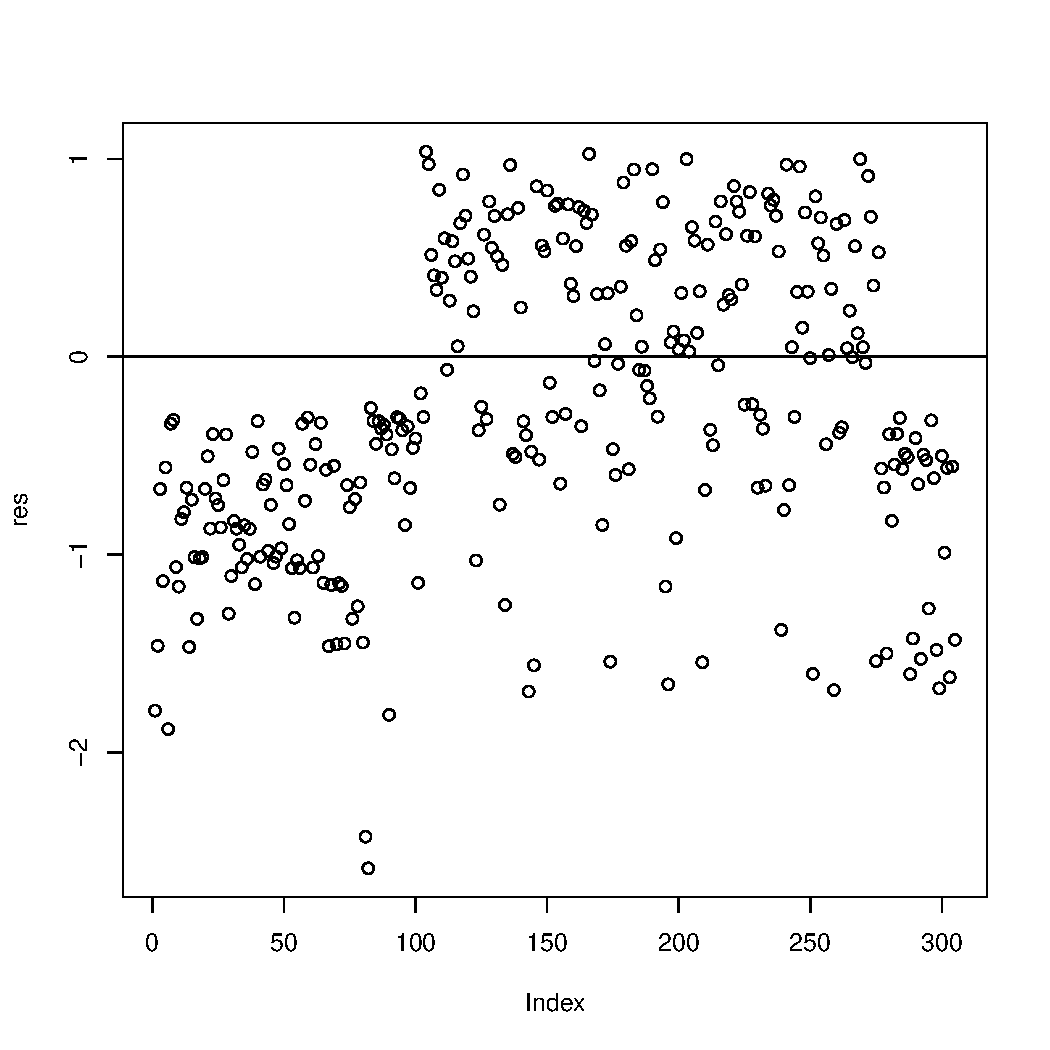
\includegraphics{A3Simulacion_files/figure-latex/unnamed-chunk-22-1.pdf}
\caption{\label{fig:unnamed-chunk-22}Autocorrelación y autocorrelación parcial para las cadenas simuladas del algoritmo MH.}
\end{figure}

\hypertarget{buenas-pruxe1cticas-en-la-aplicaciuxf3n-de-muxe9todos-mcmc}{%
\subsection{Buenas prácticas en la aplicación de métodos MCMC}\label{buenas-pruxe1cticas-en-la-aplicaciuxf3n-de-muxe9todos-mcmc}}

Dado que una gran parte de la inferencia bayesiana está ligada a la programación e implementación de los métodos MCMC para realizar inferencias posteriores de los parámetros de interés, se sugiere seguir el razonamiento y recomendaciones de \citet{GelShir2010}, que puede ser resumido en los siguientes ítemes para cada parámetro de interés:

\begin{enumerate}
\def\labelenumi{\arabic{enumi}.}
\tightlist
\item
  Simulación de tres o más cadenas de forma paralela. Los valores iniciales de cada cadena deben estar dispersos entre sí.
\item
  Comprobación de la convergencia de las cadenas mediante el descarte de la primera mitad de los valores generados en las cadenas. Esta etapa se conoce como \emph{burning stage}.
\item
  Una vez que las cadenas converjan, mezclar los tres conjuntos de valores generados por las cadenas. Esto garantiza, en primera instancia, que las cadenas no estén auto-correlacionadas.
\item
  Además de realizar esta mezcla, descartar valores intermedios mediante un muestreo sistemático. Esta etapa se conoce como \emph{thining stage}. Al final se recomienda almacenar una cantidad elevada de valores simulados.
\item
  Calibrar el algoritmo si la convergencia de las cadenas no se presenta rápidamente.

  \begin{itemize}
  \tightlist
  \item
    Para los algoritmos de Metropolis-Hastings, escoger una distribución de salto acorde con la distribución de la cual se desea simular. Por ejemplo, \citet{Cepe1} presentan dos distribuciones de salto para el problema de la modelación de la varianza (cada una de las propuestas presenta tasas de aceptación diferentes).
  \end{itemize}
\item
  Comparación y contraste de los resultados con modelos simples que permitan examinar posibles discrepancias y corregir errores de programación.
\end{enumerate}

En términos de inferencia bayesiana, se tienen dos tipos de procesos: el primero y más común, que trata de realizar inferencias acerca de un vector de parámetros de interés \(\boldsymbol \theta\); el segundo trata con los momentos del parámetro, por ejemplo su esperanza. Nótese que el primer proceso se presenta con seguridad en ejercicios empíricos simulados; sin embargo, el segundo se presenta en los ejercicios prácticos con datos reales, en donde se quiere contrastar alguna hipótesis.

Las anteriores dos opciones tienen tratamientos muy diferentes en términos de la cantidad de simulaciones requeridas. Por ejemplo, si el objetivo es inferir acerca de \(\boldsymbol \theta\), para conocer su comportamiento estructural, basta con realizar una simulación que genere una cantidad mediana de valores y que se resumen en un promedio y una desviación estándar. Por otro lado, si el objetivo es inferir acerca de \(E(\boldsymbol \theta)\), se requieren muchas más simulaciones para obtener una buena precisión. Siguiendo a \citet{GelShir2010}, una vez terminado el proceso de \emph{burning} y \emph{thining}, se sugiere que se dividan los valores simulados en las cadenas paralelas y se formen \(k\) grupos; de esta forma, una estimación de \(E(\boldsymbol \theta)\) será la gran media de las medias muestrales de cada grupo y el error estándar será su desviación estándar dividida por \(\sqrt{k}\).

\hypertarget{referencias}{%
\chapter*{Referencias}\label{referencias}}
\addcontentsline{toc}{chapter}{Referencias}

  \bibliography{book.bib}

\end{document}
